%% thesis.tex 2014/04/11
%
% Based on sample files of unknown authorship.
%
% The Current Maintainer of this work is Paul Vojta.

\documentclass{ucbthesis}
\usepackage{amsmath, amssymb}
\usepackage[natbib=true]{biblatex}
\usepackage[utf8]{inputenc}
\usepackage{graphicx}
\usepackage{bm}
\usepackage{todonotes}
\usepackage{hyperref}

\newcommand{\lcdm}{$\texrm{\Lambda}$CDM}
\newcommand{\angstrom}{\mbox{\normalfont\AA}}
\newcommand{\siliconii}{SiII $\lambda$6355}

% To compile this file, run "latex thesis", then "biber thesis"
% (or "bibtex thesis", if the output from latex asks for that instead),
% and then "latex thesis" (without the quotes in each case).

% Double spacing, if you want it.  Do not use for the final copy.
% \def\dsp{\def\baselinestretch{2.0}\large\normalsize}
% \dsp

% If the Grad. Division insists that the first paragraph of a section
% be indented (like the others), then include this line:
% \usepackage{indentfirst}

\bibliography{references}

\begin{document}

% Declarations for Front Matter

\title{Empirical Models of Type Ia Supernovae: Applications for Next-Generation Cosmological Surveys}
\author{Samantha Dixon}
\degreesemester{Fall}
\degreeyear{2020}
\degree{Doctor of Philosophy}
\chair{Professor Saul Perlmutter}
\othermembers{Professor Daniel Kasen \\
  Assistant Professor Fernando P\'{e}rez}
\numberofmembers{3}
% Previous degrees are no longer to be listed on the title page.
% \prevdegrees{B.A. (University of Northern South Dakota at Hoople) 1978 \\
%   M.S. (Ed's School of Quantum Mechanics and Muffler Repair) 1989}
\field{Physics}
% Designated Emphasis -- this is optional, and rare
% \emphasis{Colloidal Telemetry}
% This is optional, and rare
% \jointinstitution{University of Western Maryland}
% This is optional
\campus{Berkeley}

% For a masters thesis, replace the above \documentclass line with
% \documentclass[masters]{ucbthesis}
% This affects the title and approval pages, which by default calls this
% document a "dissertation", not a "thesis".

\maketitle
% Delete (or comment out) the \approvalpage line for the final version.
\approvalpage
\copyrightpage

% (This file is included by thesis.tex; you do not latex it by itself.)

\begin{abstract}

% The text of the abstract goes here.  If you need to use a \section
% command you will need to use \section*, \subsection*, etc. so that
% you don't get any numbering.  You probably won't be using any of
% these commands in the abstract anyway.

Invasive brag; forbearance.

\end{abstract}

\begin{frontmatter}

\begin{dedication}
\null\vfil
\begin{center}
To TBD \\\vspace{12pt}
For something I don't know yet
\end{center}
\vfil\null
\end{dedication}

% You can delete the \clearpage lines if you don't want these to start on
% separate pages.

\tableofcontents
\clearpage
\listoffigures
\clearpage
\listoftables

\begin{acknowledgements}
\begin{itemize}
    \item Thesis advisor: Saul Perlmutter
    \item Committee members: Bill Holzapfel (qual committee chair), Dan Kasen, Fernando Perez (filled in last minute)
    \item Senior mentors: Greg Aldering, Alex Kim
    \item Undergraduate mentors: Paolo Privitera, Al Kogut
    \item Lab mates: Kyle Boone, Kara Ponder, Ravi Gupta, Clare Saunders, Aleks Cikota, Brian Hayden
    \item Collaborators: David Rubin, Ben Rose, Rebekah Hounsell, Yu Ma
    \item Square: Deeksha Chugh, Zaki Ali, Morag Scrimgeour, Stephane Fotso, Jackie Brosamer
    \item GDSO: Mike Fang, Sumayah Rahman, James Arnemann
    \item Friends: Jeffrey Epstein, Jennet Dickinson, Tom Zick, Jessica Avva, Abi Polin
    \item Family: Parents Lisa and Fred, brother Jim, grandmother Carol
\end{itemize}

\end{acknowledgements}

\end{frontmatter}

\pagestyle{headings}

\chapter{Introduction}
\label{chap:intro}

\section{The Expansion History of the Universe}
Understanding how space has expanded over the history of the universe is key to understanding what the universe is made of, how it started, and how it may end. We start by defining the scale factor, $a$, which describes the ratio of the physical distances between objects in the past to the physical distances between the same objects today. Our quest to measure the expansion history of the universe, then, is equivalent to determining $a(t)$ -- how the scale factor evolves with cosmic time.

The cosmological principle descends from the Copernican principle: that there is nothing special about our particular viewpoint of the universe. More precisely, it states that the expansion of the universe is homogenous (the same at any point in space) and isotropic (the same in all directions). Encoding this mathematically, we can obtain the following metric, known as the Friedmann-Lema\^{i}tre-Robertson-Walker (FLRW) metric:
\begin{equation}
    ds^2 = a(t)^2\,ds_3^2 - c^2\,dt^2
    \label{eqn:flrw_metric}
\end{equation}
where $ds_3$ is the three-dimensional spatial metric and $c$ is the speed of light.

Using this metric in the Einstein field equations, we then derive the Friedmann equations, a general description of how $a$ evolves with time:
\begin{equation}
    \left(\frac{\dot{a}}{a}\right)^2 = \frac{8\pi G\rho}{3} - \frac{kc^2}{a^2}
    \label{eqn:friedmann}
\end{equation}
\begin{equation}
    \frac{\ddot{a}}{a} = -\frac{4\pi G}{3}\left(\rho + \frac{3p}{c^2}\right)
    \label{eqn:friedmann_acceleration}
\end{equation}
Dots here represent a time derivative, and $G$ is Newton's gravitational constant. The energy density, represented by $\rho$, and the energy pressure, $p$ are functions of time, like the scale factor $a$. The spatial curvature, $k$, is constant, but can take on a number of values.

To simplify our notation, we define the Hubble rate:
$$H=\frac{\dot{a}}{a}.$$
With this, the left hand side of Equation \ref{eqn:friedmann} can be replaced with $H^2$ and the left hand side of Equation \ref{eqn:friedmann_acceleration} can be replaced with $\dot{H} + H^2$.  The value of the Hubble rate today is known as the Hubble constant, $H_0$.

Assuming $k=0$ (an assumption that is experimentally justified from observations of the cosmic microwave background, see \citet{planck_collaboration_planck_2016}, for example), we can use Equation \ref{eqn:friedmann} to rewrite Equation \ref{eqn:friedmann_acceleration} as
\begin{equation}
    \dot{\rho} = -3H\left(\rho + \frac{p}{c^2}\right)
    \label{eqn:density_evol}
\end{equation}
For linear combinations of perfect fluids, each with equation of state
$$p_f = w\rho_f c^2,$$
where $w$ is known as the equation of state parameter, this equation has exact solutions of the form
$$\rho_f \propto a^{-3(1+w)}.$$
For ordinary matter, $w=0$. For radiation, $w=1/3$ and for a cosmological constant dark energy, $w=-1$. Thus, Equation \ref{eqn:density_evol} has solutions of the form:
$$\rho = \rho_m a^{-3} + \rho_r a^{-4} + \rho_\Lambda$$
Additionally, we define the critical density
$$\rho_{c} = \frac{3H_0^2}{8\pi G},$$
which describes the average energy density of a universe that would halt expansion after infinite time. Dividing the densities by this critical density gives us a unitless density parameter $\Omega$. Putting everything, together, we can obtain the relationship between the Hubble parameter and scale factor, parametrized by the time-evolving densities of the constituent components of the universe:
\begin{equation}
    H(a) = H_0\sqrt{\Omega_m a^{-3} + \Omega_r a^{-4} + \Omega_\Lambda}
    \label{eqn:hubble_vs_a}
\end{equation}
% Proof:
% $$H^2 = \frac{8\pi G}{3}\rho$$
% $$2H\dot{H}=\frac{8\pi G}{3}\dot{\rho}$$
% $$\dot{H}=\frac{4\pi G}{3H}\dot{rho}$$
% $$\dot{H} + H^2 = -\frac{4\pi G}{3}\left(\rho + \frac{3p}{c^2}\right)$$
% $$\frac{4\pi G}{3}\left(\frac{\dot{\rho}}{H} + 2\rho\right) = -\frac{4\pi G}{3}\left(\rho + \frac{3p}{c^2}\right)$$
% $$\dot{\rho} = -3H\left(\rho + \frac{3p}{c^2}\right)$$

Oftentimes, it is convenient to use the redshift, $z$, in lieu of the scale factor, since the redshift is directly observable. We define the redshift as the Doppler-like shift observed in distant objects:
\begin{equation}
    z = \frac{\lambda_o}{\lambda_e} - 1
    \label{eqn:z_def}
\end{equation}
where $\lambda_o$ is the observed wavelength and $\lambda_e$ is the emitted wavelength of some observable spectral line. The redshift we observe has a number of sources. For our purposes, the main contributors are the cosmological redshift, where the expansion of space stretches of the wavelength of emitted light causing it to appear redder, and the peculiar velocity redshift, where the motion of objects relative to us creates a Doppler shift in the observed wavelengths. Generally, when we refer to the redshift of an object, we are referring to its cosmological redshift, which is related to the scale factor by $z = 1/a - 1$. Using this definition in Equation \ref{eqn:hubble_vs_a}, we get
\begin{equation}
    H(z) = H_0\sqrt{\Omega_m (1+z)^{3} + \Omega_r (1+z)^{4} + \Omega_\Lambda}
\end{equation}

We're now in a position to begin to define some useful measures of cosmological distance, using the equations that govern the evolution of distances described above. One important distance measure for the work described here is the comoving distance, $\chi$, between an emitting object at scale factor $a$ and us ($a=1$). This distance remains constant with the universe's expansion and can be calculated by multiplying the speed of light with the aggregate of infinitesimal distances over time:
\begin{equation}
    \chi = c\displaystyle\int_{t(a)}^{t_0} \frac{dt^\prime}{a(t^\prime)}
    = -c\displaystyle\int_1^a \frac{da'}{a'^2 H(a)}
    = \frac{c}{H_0}\displaystyle\int_0^z \frac{dz'}{\sqrt{\Omega_m(1+z')^3 + \Omega_r(1+z')^4 + \Omega_\Lambda}}
\end{equation}

The angular diameter distance describes the ratio of an object's physical size to its angular size on the sky, and is related to the comoving distance by
$$d_A(z) = \frac{\chi(z)}{1+z}$$

Finally, we have the most important distance measure for our work: the luminosity distance. This distance defined by
\begin{equation}
    d_L(z) = \sqrt{\frac{L}{4\pi F}}
    \label{eqn:luminosity_dist}
\end{equation}
where $L$ is the luminosity of an object and $F$ is the flux (or observed brightness) of the object. Interestingly, it can be shown that this quantity is equivalent to \footnote{The full proof of this equivalence (known as the Etherington reciprocity theorem) is quite complicated. However, we can obtain this relation by noting that the surface brightness of an object is reduced by a factor of $(1+z)^{-4}$ as it recedes, while the angular area decreases as $d_A^{-2}$ \cite{hogg_distance_1999}.}
\begin{equation}
    d_L(z) = (1+z)^2 d_A(z) = (1+z)\chi(z).
    \label{eqn:luminosity_dist_z}
\end{equation}


In astrophysical contexts, it is common to work in logarithmic-scale magnitudes. This leads to the definition of the distance modulus, $\mu$, defined as the difference between the apparent magnitude of an object, $m$, and its absolute magnitude, $M$, which is itself defined as the apparent magnitude of an object if it were seen from a distance of 10 parsecs. The distance modulus is therefore related to the luminosity distance by
\begin{equation}
    \mu = m - M
    = -2.5 \log_{10}\left[\frac{F(d_L)}{F(d_L = 10\textrm{ pc})}\right] = 5 \log_{10}\left(\frac{d_L}{10\textrm{ pc}}\right) - 5
    \label{eqn:distmod}
\end{equation}

\section{Using Standard Candles to Constrain Cosmological Parameters}
A classic method for obtaining estimates of the luminosity distance is to observe standard candles. A standard candle is any class of astronomical objects that has a known intrinsic luminosity. By observing the apparent brightness of these objects, we directly obtain the luminosity distance as defined in Equation \ref{eqn:luminosity_dist} (or equivalently the distance modulus as defined in Equation \ref{eqn:distmod}). We can also use spectral observations of these objects or their host galaxies to compare the observed frequencies of various emission and absorption lines in the spectrum to the known frequencies of these lines in order to calculate each object's redshift, as in Equation \ref{eqn:z_def}. Combining these measurements gives us the Hubble-Lema\^{i}tre diagram, a plot of luminosity distance (or equivalently the distance modulus) as a function of redshift. Different cosmological models predict different relationships between distance and redshift, so our standard candle observations can be used to differentiate between and constrain the parameters of different theoretical models. In Figure \ref{fig:hubble_diagram_examples}, we show a few examples of distance-redshift relations for different cosmological models.

\begin{figure}[htpb]
    \centering
    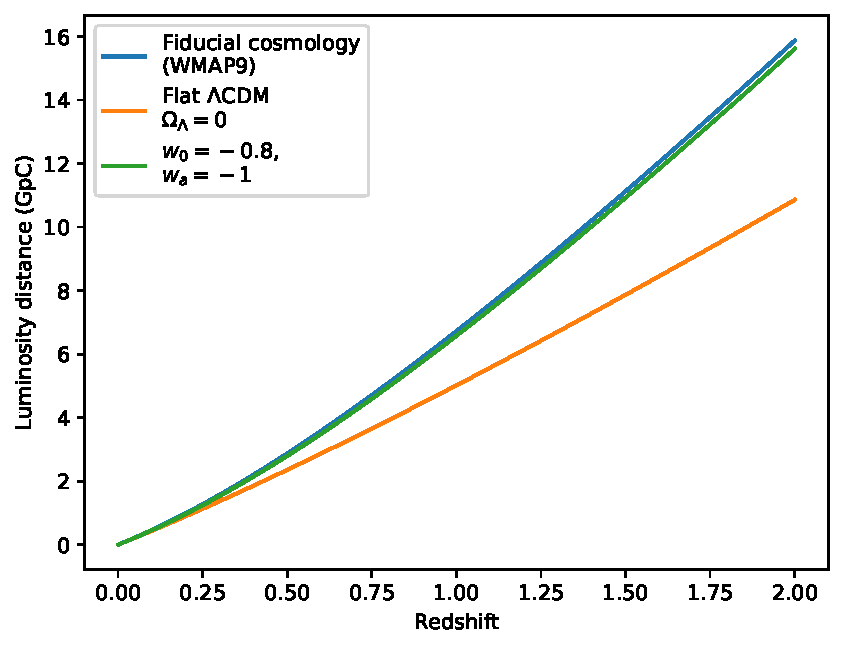
\includegraphics{figures/intro/hubble_diagram_examples.pdf}
    \caption{Hubble-Lema\^{i}tre diagrams for different cosmological models. In blue, we have a fiducial, flat $\Lambda$CDM cosmology with density parameters matching those determined by \citet{komatsu_five-year_2009}. In orange, we show another flat $\Lambda$CDM cosmology, but dominated entirely by matter (i.e. $\Omega_\Lambda=0$). In green, we show an example of the distance-redshift relation for an alternate parametrization of dark energy with a varying equation of state parameter.}
    \label{fig:hubble_diagram_examples}
\end{figure}

The standard cosmological model is the flat, $\Lambda$CDM model, which posits that the spatial curvature of the universe is flat ($\Omega_k=0)$, and that the energy density is composed primarily of dark energy that behaves as a cosmological constant, followed by cold dark matter, and finally ordinary baryonic matter. This model is supported by the findings of a number of different probes \citep{planck_collaboration_planck_2016, wittman_detection_2000, eisenstein_detection_2005}. Its Hubble-Lema\^{i}tre diagram is shown in blue in Figure \ref{fig:hubble_diagram_examples}, where we have take the density parameter values from \citet{komatsu_five-year_2009}: $\Omega_\Lambda = 0.7135$ and $\Omega_m = 0.2865$. We can see that the distance-redshift relation for this cosmology differs significantly from a similarly parametrized cosmology but with $\Omega_\Lambda=0$ and $\Omega_m=1$ (seen in orange in Figure \ref{fig:hubble_diagram_examples}).

$\Lambda$CDM is not the only cosmological model. One popular alternate model envisions dark energy as a dynamical scalar field, rather than a cosmological constant. In this case, the equation of state parameter $w$ of dark energy is allowed to vary with redshift (or equivalently, scale factor). This variation can be parametrized by
\begin{equation}
    w(a) = w_0 + w_a(1 - a) = w_0 + w_a z/(1+z)
\end{equation}
(see \citet{chevallier_accelerating_2001} or \citet{linder_exploring_2003}). A cosmological constant can be encapsulated in this parametrization by setting $w_0=-1$ and $w_a=0$, so deviations from these values would serve as useful clues as to the precise nature of dark energy. An example distance-redshift relation with $w_0=-0.8$ and $w_a=-1$ is shown in green in Figure \ref{fig:hubble_diagram_examples}. We can see that the difference in the current fiducial cosmology distance-luminosity relationship and that of this alternate cosmology is quite small, but increasing with redshift. In order to constrain the parameters of these alternate models, we need to have extremely precise measurements of the luminosity distance, and also be able to extend these measurements further back in time (i.e. to higher redshift).

\section{Type Ia Supernovae as Standardizable Candles}
\label{sec:standardizable_candles}
Type Ia supernovae (SNe Ia), exploding carbon-oxygen white dwarfs in binary systems, are excellent standard candle candidates. They are observed to have very similar intrinsic brightnesses. Moreover, they are extremely bright — about 5 billion times brighter than the Sun — so they can be seen out to large distances, and therefore probe earlier epochs of cosmic history. SNe Ia were instrumental in discovering that the expansion rate of the universe is accelerating, and they remain one of the best tools we have for constraining the properties of the dark energy that drives this accelerating expansion \citep{perlmutter_measurements_1999, riess_observational_1998}.

While Type Ia supernovae do have similar intrinsic brightnesses, they are not perfect standard candles. The scatter in their peak absolute magnitudes is $\sim 40$\%. They are, however, standardizable candles; that is, their peak brightnesses are strongly correlated with other observable properties of the explosion.

One of these observables is the light curve width (sometimes referred to as the decline rate), a measure of how quickly the event brightens and fades. SNe Ia with broader light curves tend to be intrinsically brighter. The relationship was first shown empirically in the 1970s \citep{rust_use_1974, pskovskii_light_1977} and later refined with additional observations and extending out to higher redshifts \citep{phillips_absolute_1993, hamuy_morphology_1996, perlmutter_measurements_1997}. The color of the supernova is also known to correlate with the brightnesses of SNe Ia -- bluer objects tend to be brighter. The width-luminosity relationship is theoretically explained as being due to differences in the opacity due to temperature differences \citep{kasen_origin_2007}. The color-luminosity relationship is not yet well-explained theoretically, but has been reproduced in a number of theoretical models \citep[e.g.][]{kasen_diversity_2009}. \citet{tripp_two-parameter_1998} introduced the combined correction for both width and color, enabling Type Ia supernova magnitudes to be standardized to within approximately 0.15 magnitudes, and similar relationships have been used in models like the multicolor light curve shapes model \citep[MLCS,][]{riess_precise_1996}.

Currently, the conventional method for standardization involves fitting observed broadband light curves with the SALT2 model of \citet{guy_salt2_2007} in order to obtain measurements of the light curve width and the color. SALT2 does not directly measure the light curve width or color like previous methods, which use parameters like $\Delta m_{15}$, the decrease in Bessell B-band magnitudes from maximum light to 15 days after maximum. Instead, the model parametrizes the full evolution of the spectral fluxes of Type Ia supernovae as follows:
\begin{equation}
    f(\lambda, p) = x_0\left(M_0(\lambda, p) + x_1 M_1(\lambda, p)\right) \times \exp [c\times\textrm{CL}(\lambda)]
    \label{eqn:salt_flux}
\end{equation}
where $\lambda$ represents wavelength and $p$ is the number of rest-frame days after maximum brightness (also known as the phase). $M_0$ and $M_1$ are fixed spectral sequences that describe the mean spectral evolution of SNe Ia and their major sources of spectral variation, respectively. $\textrm{CL}(\lambda)$ is a fixed description of the color variation that remains fixed across phases, and includes contributions from both intrinsic color differences and color differences due to host galaxy dust extinction. This model can be thought of as akin to a principal component decomposition of SN Ia spectral evolution, with $x_0$, $x_1$, and $c$ indicating where each supernova is located in the model basis and representing each supernova's overall brightness, light curve width, and redness, respectively. Using such parametrization avoids systematic errors from K-corrections that stem from large variations in spectral features.

After using the model to fit each supernova in a given data set, we typically standardize their observed brightnesses using a modified version of the Tripp relation:
\begin{equation}
    \mu = m_B^* - M + \alpha \times x_1 - \beta\times c
    \label{eqn:standardization}
\end{equation}
where $m_B^*$ is the apparent B-band magnitude calculated from the best-fit model parameters $x_0$, $x_1$, and $c$ for each supernova and $\mu$ is the distance modulus to each supernova. $M$, $\alpha$, and $\beta$ are global parameters that describe the overall standardized absolute magnitude in the  Bessell B-band, the light curve shape-luminosity relation, and the color-luminosity relation, respectively. Typically, we start by assuming some fiducial cosmology that defines a distance $\mu_\text{cosmo}$, and we fit the global standardization parameters $M$, $\alpha$, and $\beta$ by minimizing the $\chi^2$ defined by
\begin{equation}
    \chi^2 = (\mu - \mu_\text{cosmo})^T C^{-1} (\mu - \mu_\text{cosmo}),
    \label{eqn:chi2_cosmo_full_cov}
\end{equation}
where $C$ defines the covariance matrix between SN Ia observations. Then by fixing these values of $M$, $\alpha$, and $\beta$, we can perform a similar $\chi^2$ minimization that finds the best-fit cosmological parameters. The process repeats until convergence.

Alternatively, the UNITY framework \citep{rubin_unity_2015} performs this standardization and cosmology fit from light curve parameters with a fully Bayesian approach. In this case, the nuisance parameters and cosmological parameters, as well as their full posterior distributions, are obtained using Hamiltonian Monte Carlo techniques.

Regardless of the method of fitting, the residuals on the Hubble diagram (i.e. the differences between the distance moduli obtained from the best standardization of the light curve parameters and the distance moduli predicted by the best-fit cosmological parameters) still have a root-mean-square (RMS) dispersion of approximately 0.15 magnitudes. Some of this dispersion can be explained by the measurement, calibration, and model uncertainties of the photometry and light curve model fitting process. However, some amount of the dispersion (typically about 0.10 magnitudes) remains unexplained.

\section{SN Ia Standardization Beyond SALT2}
The remaining unexplained dispersion in standardized supernova magnitudes from using SALT2 and the Tripp relation indicates that there may be more progress to be made in SN Ia standardization. One method to make such an improvement is to look for additional parameters that correlate with the remaining variation and using these to correct the residuals further. \citet{kelly_hubble_2010} and \citet{sullivan_dependence_2010} found evidence of such a correlation between the host galaxy mass of supernovae and their Hubble residuals. Because of this, it is now standard to see supernova cosmology analyses include a correction term in their distance moduli calculations to account for this correlation. It has also inspired the search for other corrections to supernova magnitudes stemming from the supernova environment, like examinations of the global (entire galaxy) or local specific star formation rate \citep{rigault_evidence_2013, rigault_confirmation_2015}.

Some of these additional parameters are measured from the supernovae themselves, rather than their environments. A number of studies have searched for correlations between supernova spectral features and their absolute luminosities. \citet{nugent_evidence_1995} first outlined the existence of a spectroscopic sequence that relates the ratios of the depths of the \ion{Si}{ii} $\lambda$6355 and \ion{Si}{ii} $\lambda$5972 lines and the ratios of the \ion{Ca}{ii} H\&K lines to the absolute magnitude. \citet{bailey_using_2009} used the ratio of the absolute fluxes at two specific wavelengths to improve the standardization beyond what was possible with the Tripp standardization. Other studies have attempted to subclassify Type Ia supernovae using spectral indicators like the width of the \ion{Si}{ii} $\lambda$6355 and \ion{Si}{ii} $\lambda$5972 lines \citep{branch_comparative_2006}, or the ejecta velocity as measured by the blue shift of the minima of these lines \citep{wang_improved_2009, foley_measuring_2011, foley_relation_2012}. By using different corrections for these subclasses, these studies have shown some improvements to the standardization precision.

An alternate approach is to create more flexible light curve or spectral models. This is the tack taken by the SNEMO models \citep{saunders_snemo_2018}. SNEMO extends the logic of SALT2 by modeling the full spectral time series evolution of SNe Ia fluxes with additional components beyond the light curve shape captured by SALT2's $x_1$ parameter. The SNEMO flux model is
\begin{equation}
    f(\lambda, p) = c_0\left[e_0(\lambda, p) + \displaystyle\sum_{i=1}^k c_i\times e_i(\lambda, p)\right] \times \exp\left[A_s\times \textrm{FM07}(\lambda)\right]
\end{equation}
where $\textrm{FM07}$ is the \citet{fitzpatrick_analysis_2007} dust extinction law. The functional form of this equation is quite similar to that of Equation \ref{eqn:salt_flux}, however the number of linear components, $k$, is not fixed to one. SNEMO encompasses three separate models, each varying in the number of linear components that are used, and each intended for different uses. SNEMO2 ($k=1$) is useful as a comparison to the typical light curve shape and color models like SALT2, as the training methodology is slightly different from that of SALT2. SNEMO15 ($k=14$) was introduced as a model that captures as much of the spectral variation that exists in Type Ia supernovae without overfitting. The SNEMO7 model is intended as an intermediate model that can best standardize SN Ia magnitudes, using an extension of the Tripp relation:
\begin{equation}
    \mu = m_B - \left(M + \beta A_s + \displaystyle\sum_{i=1}^k \alpha_k \; c_k\right)
\end{equation}
The resulting dispersion with this parametrization is approximately 0.113 mag, of which 0.097 magnitudes are not explained by the measurement error. Thus, by extending the model used to describe supernova spectral variation, SNEMO is able to improve the standardization precision.

The SUGAR model presented in \citet{leget_sugar_2020}, effectively combines both approaches -- using spectral feature measurements as an alternate parametrization of a full spectral time-series model. Rather than performing a principal component decomposition of the full, interpolated, spectral time-series data (like SNEMO), SUGAR first measures a series of spectral indicators in the near-maximum spectra. Then, a PCA decomposition of these indicators is used to obtain a 4-dimensional projection vector corresponding to each supernova in the data set. Finally, the full spectro-temporal model is created by fitting for basis functions like the $e_i(\lambda, p)$ of SNEMO that, when linearly combined with the spectral indicator projections, accurately predict the spectral evolution of the supernovae. The SUGAR model does not yet have a corresponding standardization model, so we do not yet have an estimate of how well we can correct the brightnesses of supernova for the effects captured by the SUGAR model. However, the model is able to capture much more of the spectral variation in SNe Ia than SALT2, without a large increase in the number of parameters in the model.

So far, all of the methods discussed have been parametric and model both the spectral evolution (besides color) and the relation between SN parameters and SN absolute luminosities linearly. The work of \citet{fakhouri_improving_2015} takes a non-parametric approach, directly comparing the spectra of supernovae to identify pairs of ``twins," i.e. supernovae with nearly identical spectral time-series data, up to a difference in host-galaxy dust extinction and apparent magnitude. They found that the best pairs of twins differed in absolute magnitude on average by only $0.083 \pm 0.012$ mag (and by only $0.072 \pm 0.010$ mag after accounting for peculiar velocities). This implies that a direct comparison of the spectra, without any intermediate parametrization and modeling of necessary corrections, could produce better standardization.

\citet{boone_twins_2020a} sought to understand the mathematical structure of the ``twinness space" amongst near-maximum-brightness spectra. First, they estimated the aspects of the spectral variation that were due to differences in dust extinction and the overall brightness difference. Then, using the at-max spectra corrected for the differences in brightness and extinction, they applied the Isomap algorithm \citep{tenenbaum_global_2000} to find a low-dimensional representation of the remaining spectral variation that approximately preserves the twins distances from \citet{fakhouri_improving_2015}. The low-dimensional embedding faithfully reconstructs many of the previously discussed spectral indicators of supernova diversity. Furthermore, \citet{boone_twins_2020b} presents an additional model that predicts the variation in a supernova's brightness based on its location in the ``twins embedding." Using this technique, they were able to standardize the supernovae in the sample to within $0.084 \pm 0.007$ mag, a level comparable to the best twins comparison of \citet{fakhouri_improving_2015}, but with a parametric approach.

\section{Open Questions in Supernova Cosmology}
\subsection{Optimal Parametrization of SNe Ia}
We could see in the previous section that there has been much work put into the development of empirical models of Type Ia supernova spectral variation and evolution, including linearly parametrized models of the full spectral evolution (SALT2, SNEMO, SUGAR), non-parametric comparisons between at-max spectra (twins), and nonlinear parametrizations of at-max spectra (twins embedding). Each of these models attempts to find a low dimensional representation of the extremely complex spectral and temporal evolution of stellar explosions. However, it is not yet clear precisely how this dimensionality reduction should be accomplished.

\citet{rubin_constraining_2020} addresses one aspect of this question: estimating the optimal dimensionality of the latent parameteric space. Using counting statistics of the twin pairings found in \cite{fakhouri_improving_2015}, along with the insight from geometry that volumes concentrate on surfaces, \citeauthor{rubin_constraining_2020} argues that the ideal parameteric SN Ia model has about 3-4 parameters, excluding color. This number squares with the findings of \citet{boone_twins_2020a}, which found that a non-linear 4-dimensional parameter space describes the near-maximum brightness spectral variation of SNe Ia, as well as with the SUGAR model, which found that 4 parameters were sufficient to model most of the variation in near-maximum spectral indicators.

This is however smaller than the 7 parameters of SNEMO7, which was found to best standardize supernovae when assuming a linear relationship between these parameters and the absolute magnitudes of supernovae, and the 15 parameters of SNEMO15 that were found to best capture the full diversity of the supernova spectral behavior. Having such high-dimensional models can also prove problematic when we don't have high quality spectrophotometry -- \citet{rose_initial_2020} found that it is difficult to constrain even 7 parameters with currently available photometric measurements. SUGAR's ability to capture most spectral variation with four parameters suggests that changing the way we determine the linear basis we use to describe supernovae may be of use in improving standardization using data that is already in hand. However, there is not yet a standardization model for SUGAR, i.e. a mapping from a supernova's location in parameter space to its absolute brightness, so it is not yet clear if this alternate basis is effective in the final standardization step.

The fact that the twinning techniques of \citet{fakhouri_improving_2015} and \citet{boone_twins_2020b} can standardize brightnesses so precisely may point to the idea that a non-linear standardization model may be part of the solution to the puzzle of the ideal description of Type Ia supernovae for cosmology. Some evidence for this non-linearity has already been seen; \citet{rubin_unity_2015} found a preference for a piecewise linear color-luminosity relationship, and \citet{kim_standardizing_2013} found that using a Gaussian process regression of light curve parameters can in some circumstances give better standardization results.

Additionally, the fact that the twins studies achieve such good standardization using only single spectra near maximum brightness may indicate that there is no need to observe the full spectral evolution (or even broadband evolution) of Type Ia supernovae to standardize them; all of the necessary information could be encoded in a single spectrum. However, obtaining these spectra may be prohibitively expensive, and it may be difficult to properly schedule observations to ensure that the spectra obtained are within the window of phases that enable these techniques. More work is needed to understand the trade-offs involved in using these alternate methods.

Each of the empirical models that have been developed have their merits and their pitfalls. There remains much work to be done in fully comparing the models to one another, in understanding how each model performs when using different types of data with varying quality, and in using the lessons learned in the construction and study of these models to inform new models. Some of this work will be presented here.

\subsection{Population Drifts with Redshift}
Many of the standardization methods we have discussed make the implicit assumption that the corrected magnitudes of SNe Ia are identical regardless of redshift, and that any unmodeled variation is due to processes that remain stable across redshift. These assumptions may not necessarily hold, if, for example, the standardized magnitude is related to the metallicity of the supernova progenitor star, or if dust properties change throughout cosmic history. If these trends are not recognized and modeled, we will have a biased Hubble-Lema\^{i}tre diagram, and thus have biased estimates of cosmological parameters.

It is imperative that when we are designing future surveys (like LSST or the Roman Space Telescope), we are prepared to catch and correct for this type of drift. Using the twins method of \citet{fakhouri_improving_2015} may allow us to avoid the issue entirely, since that technique uses direct comparisons rather than modeling corrections to the observed magnitudes. However, as we have emphasized, using this technique requires high quality spectrophotometric observations of SNe Ia. There may still exist more efficient means of determining the twin-like subclassification of SNe Ia so that we can use them in this type of like-to-like direct measurement of relative distances. Alternatively, we can use existing parametric models to simulate the types of data that we could obtain from these future surveys, given the relevant instrument and observing parameters. Using more flexible models can allow us to get a better sense of how sensitive these future measurements will be to drifting population parameters, and, in so doing, better inform our survey design decisions.

\subsection{Hubble Constant Discrepancy}
In addition to understanding the evolution of the rate of expansion of the universe, we would also like to quantify its current value, the Hubble constant, $H_0$. Type Ia supernovae cannot be used directly for this measurement, as they are relative distance indicators, not absolute distance indicators. However, more fundamental distance calibration measurements are only possible using very nearby objects, where the distance-redshift relation is dominated by peculiar velocities. To overcome this issue, we can use the nearby fundamental measurements to calibrate a series of increasingly distant relative distance indicators until we reach the Hubble flow, where peculiar velocities are no longer dominant. This technique is usually referred to as the distance ladder.

The value of the Hubble constant can also be determined by using measurements of the cosmic microwave background (CMB) to calibrate the length scale of fluctuations in the matter density in the universe. This length scale is embedded in both the CMB and the visible matter density due to a preferred length scale in acoustic waves in the primordial plasma of the universe, (baryon acoustic oscillations, or BAO).

\citet{riess_24_2016} and \citet{riess_large_2019} used this first method to measure $H_0$, taking a geometric distance to the Large Magellanic Cloud (LMC) determined by observations of detached eclipsing binaries to calibrate the period-luminosity relationship of Cepheid variable stars, and using the distances determined from Cepheids to calibrate Type Ia supernovae. They found $H_0=74.03 \pm 1.42$ km s$^{-1}$ Mpc$^{-1}$. However, using CMB measurements and assuming a $\Lambda$CDM cosmology, \citet{planck_collaboration_planck_2016} found a value of $H_0=67.27 \pm 0.60$ km s$^{-1}$ Mpc$^{-1}$. There is thus a $4.4\sigma$ discrepancy between the value of the Hubble constant measured using probes of the late universe (geometric distances, Cepheids, supernovae) and the value measured using probes of the early universe (CMB, BAO).

Some additional methods for determining the value of $H_0$ have been introduced, including using stars at the tip of the red giant branch in the Hertzsprung-Russell diagram in a galaxy to determine a distance to that galaxy \citep{freedman_calibration_2020}, using gravitationally-lensed quasars \citep{bonvin_h0licow_2017}, or combining simultaneous observations of electromagnetic and gravitational wave to obtain distances from so-called ``standard sirens" \citep{holz_using_2005}. None of these techniques, however, have yet been able to conclusively resolve this dispute.

The tension in the values of $H_0$ may suggest the existence of new physics beyond the $\Lambda$CDM paradigm. However, it may also simply suggest the existence of a systematic bias in the techniques used to make these measurements. Understanding the systematic errors inherent in the Type Ia supernova standardization process and analysis is therefore necessary to fully understand and resolve this tension.

\section{Dissertation Outline}
In this dissertation, we present work that addresses some of these outstanding questions approached from a number of different angles. Each of these questions and studies may seem disparate, but they are all on some level connected by a larger theme: the need to identify, quantify, and mitigate systematic errors and potential bias in upcoming supernova surveys. In the age of large supernova surveys like the Rubin Observatory and Roman Space Telescope, the number of supernovae observed will be large enough that the statistical error on our distance estimates will be subdominant to the error stemming from systematic biases. Therefore, identifying the sources of bias, whether from detector-level effects (Chapter 2) or final analysis techniques (Chapter 5), is essential to ensuring the continued success of supernovae as probes of cosmic expansion. There is also a need to understand the impact that these errors can have on our final measurements after including observational effects like spectral resolution, temporal cadence, or signal-to-noise ratio. This motivates both an exploration of how much information can be extracted from different types of observations (Chapters 3, 4, and 6), as well as the creation of simulations that are representative of the wide range of behaviors that have been studied in SNe Ia (Chapter 4 and the later portions of Chapter 6).

Chapter 2 focuses on a measurement of a particular detector-level effect (charge transfer efficiency, or CTE). This effect is caused by ``traps" in the silicon lattice of the charge-coupled device (CCD) detectors that are ubiquitous in optical astronomy. These traps delay the readout of the photoelectron signal in the detector array leading to visible trails in the resulting images. The smearing from charge transfer inefficiency is particularly problematic in spectroscopic contexts, as the trails often align with the dispersion axis of the images that are processed into spectra, confusing this detector smearing with, for example, physical spectral feature broadening. In this chapter, we use two different techniques to quantify the CTE in each of the detectors on the SuperNova Integral Field Spectrograph (SNIFS), the instrument that collected much of the data used in the remaining chapters.

Chapter 3 investigates a particular spectral region of Type Ia supernovae (encompassing the \ion{Si}{ii}$\lambda$5972 and \ion{Si}{ii}$\lambda$6355 features) near maximum brightness and presents a model that is able to extract accurate measurements of the location (velocity) and size (equivalent width) of these spectral features from spectra with lower signal-to-noise ratios and lower resolution. This region of the spectrum is frequently used in some of the subclassification schemes of SNe Ia mentioned in Section \ref{sec:standardizable_candles}, and can also serve as a proxy for identifying changes in populations of certain subtypes of SNe Ia with redshift. Enabling the use of lower quality spectra is key to monitoring potential population drifts (and therefore mitigating systematic bias) at higher redshifts, allowing us to probe even earlier eras of cosmic history.

We investigate a more general approach to a similar problem in Chapter 4. There, we examine how well two existing linear empirical models of Type Ia supernova evolution (SALT2 and SNEMO) can capture a variety of near-maximum spectroscopic features (including the region studied in Chapter 3). We also provide a model for producing realistic fake spectra. The former study aims to begin exploring how well the inclusion of additional linear components to spectral models can capture non-linear features like ejecta velocities. The latter portion enables future studies that use spectral templates that capture the full range of supernova spectral behavior.

Chapter 5 addresses a general statistical problem that appears in a number of supernova standardization analyses. Supernova analyses will perform a fairly standard linear regression (see Equation \ref{eqn:standardization}), using a few covariates (e.g light curve parameters) to predict some target values (e.g. absolute magnitude). Then, they will perform a second regression, using an additional covariate (e.g. host galaxy stellar mass) to predict the residual from the initial regression. We show that that this practice is statistically sound if the covariates in the initial regression are not correlated with the covariates used in the second regression. However, these correlations do frequently exist in the studies that use this analysis workflow, and thus their results may be biased. We calculate closed-form solutions for the magnitude of these biases for a toy model of the problem, and also measure the size of this bias in the context of supernova standardization using publicly available data sets.

Finally, in Chapter 6, we present two new models of Type Ia supernova spectroscopy that make use of deep learning techniques, which we name \texttt{spec2embed} and \texttt{embed2spec}. Both of these models can be viewed as temporal extensions of the ``twins embedding" models presented in \citet{boone_twins_2020a} and \citet{boone_twins_2020b}. The \texttt{spec2embed} model uses single spectra, observed at any phase from -10 to +40 days after maximum brightness, to accurately predict both the phase of the spectrum and the location of the supernova that the spectrum came from in the twins embedding space. This allows us to perform comparably accurate standardization, and hence distance determination, using a wider range of spectra. Aside from extending the usefulness of the spectral embedding found by \citet{boone_twins_2020a}, the success of the \texttt{spec2embed} model in predicting the embedding coordinate across phases may also suggest that the spectral information content that determines the absolute magnitude of a Type Ia supernova is not restricted to observations near maximum brightness. The \texttt{embed2spec} model reverses this process, predicting the spectrum of a supernova given its location in the twins embedding space and its phase. This model enables a forward-modeling approach to fitting, allowing us to constrain the location of a newly observed object using multiple spectra, spectra with lower spectral resolution, or even broadband photometry. We conclude with some suggestions for future studies that apply these new models.

\chapter{Measurements of Charge Transfer Efficiency in the SNIFS Detectors}

\section{Introduction}
Traps in the silicon lattice of the CCD can capture charge and release it at a later time. The trapped and released charge can result in smearing of point sources along the direction of charge transfer and can impede our ability to get accurate photon counts. To understand this effect, we measure the charge transfer efficiency (CTE) of the CCDs. The CTE of a CCD is the fraction of charge that survives each pixel transfer. Because CCDs used in astronomical applications make many transfers in each image, the CTE must be very close to unity, with typical values being around $1-10^{-6}$.

Because a larger number of transfers results in a higher likelihood of encountering more traps, pixels that are further from the readout register are more effected by trapped charge. This effect is especially problematic for spectroscopic instruments like SNIFS since the increased smearing with distance to the amplifier can lead to uneven broadening of spectral features.

Our goal was to quantify the charge transfer efficiency in all channels (photometric, and blue and red spectroscopic) of SNIFS using two methods. The initial characterization was done by first exposing the CCDs to a Fe-55 x-ray source to generate single-pixel events with a known spectrum and then measuring the photo-electron loss along the readout. Later, in-situ measurements were enabled by performing a similar analysis using cosmic ray events extracted from the dark frames taken during each observing run.

\section{Initial Characterization with Fe-55 X-rays}
A simple way of measuring the charge transfer efficiency of a CCD is to expose the chip to photons of a known energy. Each resulting hit on the CCD results in a known amount of charge being generated in the event. By plotting the amount of charge measured in each event vs the row number, we can see if the amount of charge that is read out decreases with increasing distance to the amplifier (a sign that the charge is being trapped along the way) and quantify this trapping.

We performed this experiment by exposing each CCD to a Fe-55 X-ray source. Fe-55 has a strong lines from K-alpha and K-beta emission at 5.9 keV and 6.2 keV, corresponding to signals in the CCD of about 1620 $\textrm{e}^-$ and 1778 $\textrm{e}^-$, respectively. Using \verb|SExtractor|, we selected all events that were 5$\sigma$ above the background. We calculated the gain, $g$, in each individual frame by fitting two Gaussians to the spectrum of fluxes, $s(f)$, extracted from these events.

\begin{equation}
    s = A_1 \exp\left(-\frac{(f-1620/g)^2}{2\sigma_1^2}\right) + A_2 \exp\left(-\frac{(f-1778/g)^2}{2\sigma_2^2}\right)
\end{equation}

\begin{figure}
    \centering
    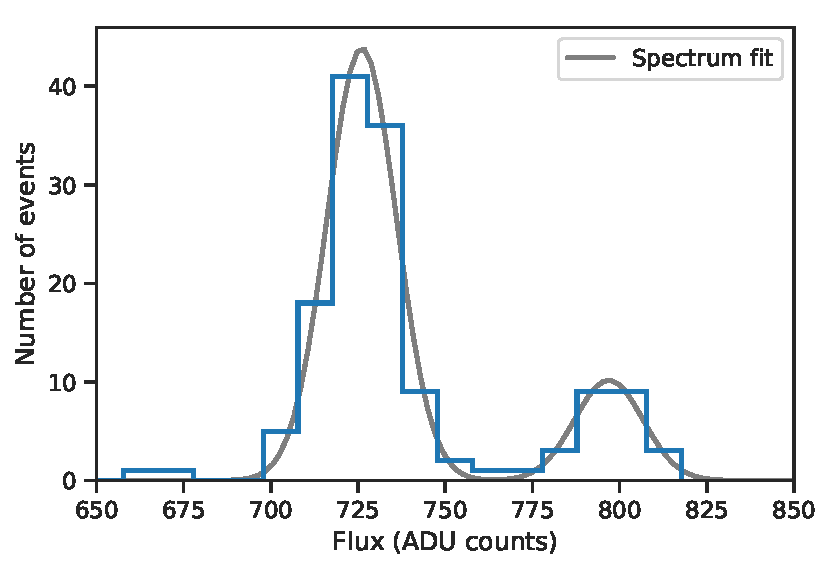
\includegraphics{figures/chap2/spectrum_fit.pdf}
    \caption{Caption}
    \label{fig:xray_spectrum}
\end{figure}

Combining the events from several X-ray frames (22 for the blue channel, 26 for the red channel, and 8 for the photometric channel), we plotted the flux for each event as a function of distance from the amplifier. By fitting a line to the data points corresponding to the K-alpha emission, we can measure how much charge is lost per transfer by dividing the slope (in units of $e^-$ per transfer) by the total number of electrons expected (1620).

The scatter plots of number of electrons vs. number of serial register transfers and number of parallel register transfers are shown in Figs. \ref{fig:cte_xray} and \ref{fig:cte_xray_serial} respectively. The resulting measurements of the charge transfer efficiency are found in Table \ref{tab:cte_xray}.

\begin{figure}
    \centering
    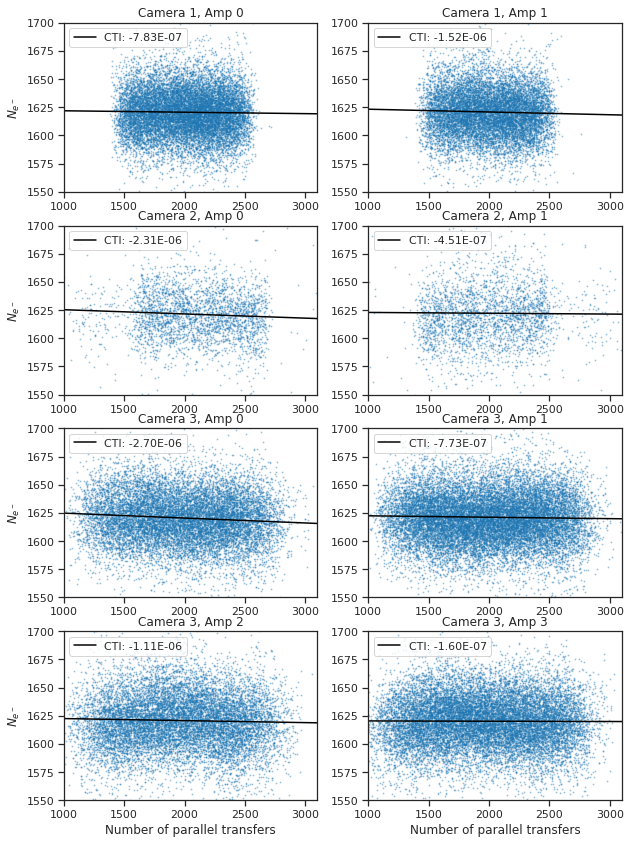
\includegraphics[width=0.9\textwidth]{figures/chap2/xray_cte_parallel.png}
    \caption{Caption}
    \label{fig:cte_xray}
\end{figure}

\begin{figure}
    \centering
    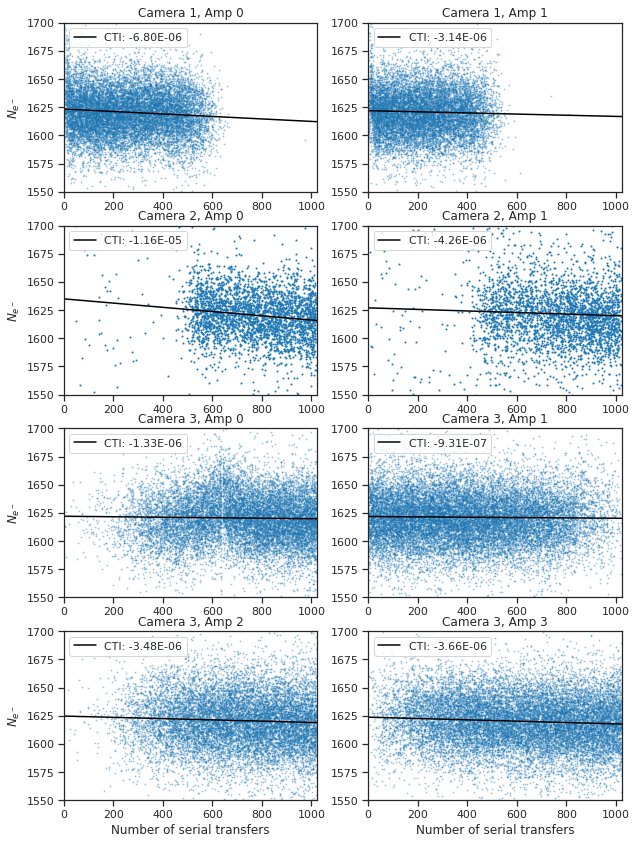
\includegraphics[width=0.9\textwidth]{figures/chap2/xray_cte_serial.png}
    \caption{Example spectrum of X-ray hits and fit to the K-alpha and K-beta emission lines.}
    \label{fig:cte_xray_serial}
\end{figure}

\begin{table}[]
    \centering
    \begin{tabular}{|c|c|c|c|c|c|}\hline
        Camera & Amp. & Parallel CTI & Serial CTI & Number of frames & Number of hits \\\hline
        B & A &0.783 $\;\pm\;$ 0.015 & 6.80 $\;\pm\;$ 0.03 & 22 & 15,925 \\
          & B &1.519 $\;\pm\;$ 0.017 & 3.14 $\;\pm\;$ 0.03 &    & 13,113 \\\hline
        R & A &2.312 $\;\pm\;$ 0.016 & 11.60 $\;\pm\;$ 0.04 & 26 & 4,071 \\
          & B &0.451 $\;\pm\;$ 0.011 & 4.26 $\;\pm\;$ 0.03 &    & 4,415 \\\hline
        P & A &2.696 $\;\pm\;$ 0.010 & 1.33 $\;\pm\;$ 0.02 & 8 & 15,308 \\
          & B &0.773 $\;\pm\;$ 0.008 & 0.93 $\;\pm\;$ 0.01 &   & 21,010 \\
          & C &1.109 $\;\pm\;$ 0.009 & 3.48 $\;\pm\;$ 0.02 &   & 14,498 \\
          & D &0.160 $\;\pm\;$ 0.008 & 3.66 $\;\pm\;$ 0.01 &   & 19,041 \\\hline
    \end{tabular}
    \caption{Charge transfer efficiency results from Fe-55 X-ray characterization. All values are in units of $10^{-6}$.}
    \label{tab:cte_xray}
\end{table}

\section{Cosmic Ray Measurement}
The X-ray measurement allows for a precise determination of the CTI if we have access to the detector. However, we'd like to be able to track changes in the CTI with time to see if there is any degradation over the course of the instrument lifetime.

By using cosmic ray hits found in dark frames, we can get an \emph{in-situ} measurement of the charge transfer efficiency on a nightly basis. 

Cosmic rays hits in the CCD do not all have the same energy, so we cannot perform the exact same analysis as we did for the X-ray tests. However, we can take advantage of the fact that charge transfer inefficiency causes smearing along the line of charge transfer along with the fact that the magnitude of this smearing increase with distance from the amplifier.

Our process is as follows:

\begin{itemize}
    \item For each dark frame taken, use \verb|SExtractor| to find cosmic ray hits. Cosmic ray hits are defined as the objects detected 1.5$\sigma$ over the noise, with a measured ellipticity $<$ 0.2 and no flags raised. Example hits are shown in Fig. \ref{fig:example_hits}. In order to avoid the noise potentially introduced by hits landing in the CTI trails of other nearby hits (see e.g. the bottom right example in Fig. \ref{fig:example_hits}), we remove from our sample all pairs of hits that are within 10 pixels of each other.
    
    \item For each cosmic ray hit, we subtract the value of the pixels above the peak (i.e. further from the readout amplifier) from the pixels below the peak. On average, this will remove the symmetric components (from oblique incidence angles and charge diffusion in the bulk silicon) from the average cosmic ray hits, leaving only the CTI trails.
    
    \item We calculate the fraction of charge in the trail by summing the number of excess counts in the 5 trailing pixels and divide it by the number of counts in the peak of the hit
    
    \item By plotting the median fraction of charge lost to CTI as a function of distance from the readout amplifier and fit a line to the data. The slope of the line gives us a measure of the charge transfer inefficiency.
    
\end{itemize}

\begin{figure}
    \centering
    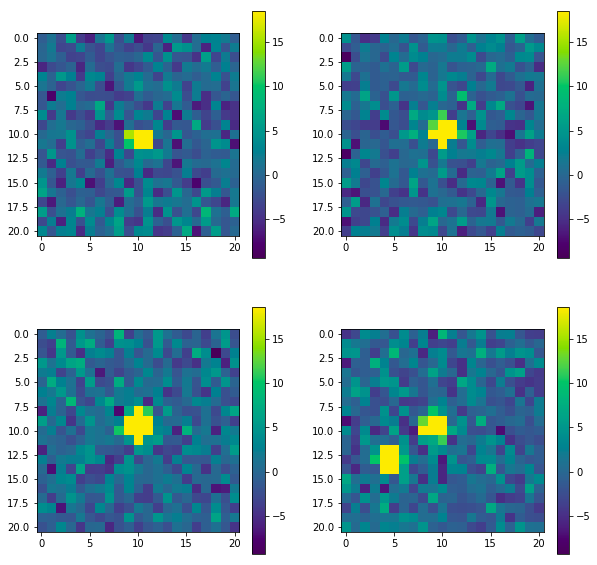
\includegraphics[width=0.9\textwidth]{figures/chap2/example_hits.png}
    \caption{Example identified cosmic ray hits passing our ellipticity cut. The two neighboring hits seen in the bottom right example would be removed from the final sample because they are too close to each other. This culling removes some of the noise from our final signal.}
    \label{fig:example_hits}
\end{figure}

We aggregate these measurements on a nightly basis. Fig. \ref{fig:cte_single_night} shows the fraction of counts lost to CTE as a function of distance to the amplifier in each amplifier for a single night.

\begin{figure}
    \centering
    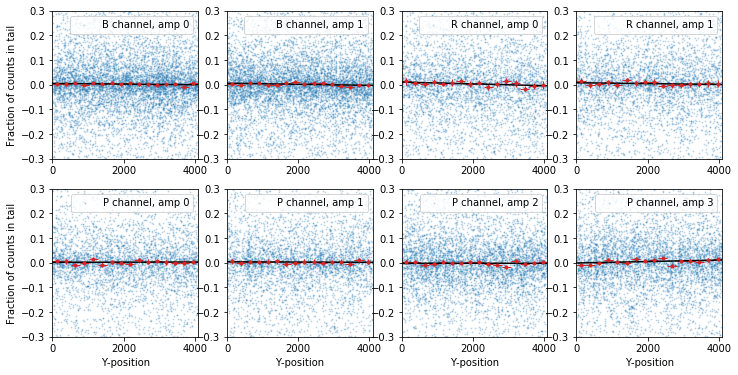
\includegraphics[width=0.9\textwidth]{figures/chap2/single_night_example_parallel.png}
    \caption{Example measurement of CTI from cosmic ray tails from a single night. All blue dots represent a single cosmic ray hit. The red points show the median fraction of counts in the peak of the hits to end up in the tails in each y-position bin. The best-fit line is also shown. The slope of this line gives us the CTI.}
    \label{fig:cte_single_night}
\end{figure}

We repeat these measurements for every night in order to check for time dependence. In Fig. \ref{fig:time_variation} we show the CTI as a function of time for each amplifier. There is very little evidence of significant degradation over time.

\begin{figure}
    \centering
    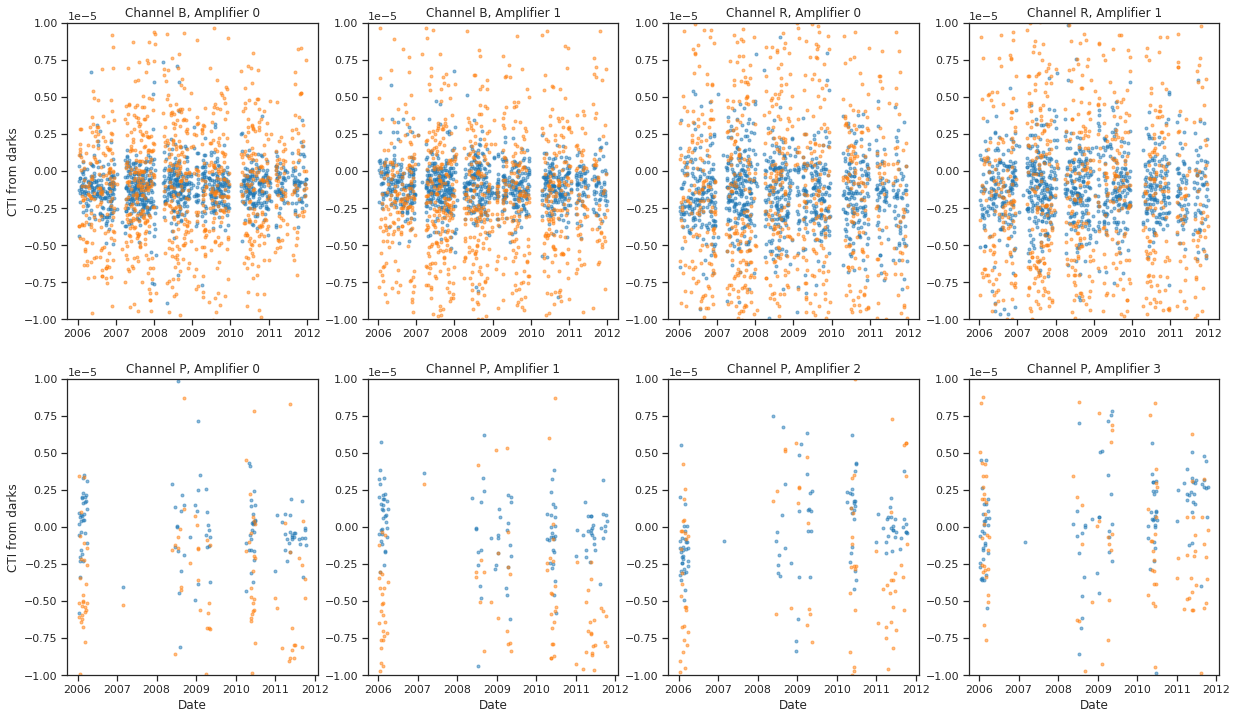
\includegraphics[width=0.9\textwidth]{figures/chap2/time_variation.png}
    \caption{A search for potential time variation in the charge transfer efficiency of each of the spectroscopic cameras. No time variation is visible.}
    \label{fig:time_variation}
\end{figure}

The average CTI numbers for each amplifier are summarized in Table \ref{tab:cte_darks}.
\begin{table}[h!]
    \centering
    \begin{tabular}{|c|c|c|c|}\hline
        Camera & Amplifier & Median Parallel CTI  & Median Serial CTI \\ \hline
        B & A &   1.08 $\pm$ 0.04  &  0.96 $\pm$ 0.13 \\
          & B &   0.97 $\pm$ 0.04  &  2.02 $\pm$ 0.13 \\\hline
        R & A &   1.49 $\pm$ 0.07  &  2.4  $\pm$ 0.2 \\
          & B &   1.24 $\pm$ 0.07  &  2.3  $\pm$ 0.2 \\\hline
        P & A &   0.19 $\pm$ 0.18  &  5.1  $\pm$ 0.5 \\
          & B &   0.18 $\pm$ 0.19  &  7.0  $\pm$ 0.4 \\
          & C &   0.3  $\pm$ 0.2   &  5.4  $\pm$ 0.7 \\
          & D &   0.5  $\pm$ 0.2   &  1.9  $\pm$ 0.5 \\\hline
    \end{tabular}
    \caption{Distribution of CTI measurements over time from all dark frames collected from 2006 to 2012.}
    \label{tab:cte_darks}
\end{table}

% \begin{deluxetable}{lcD@{$\ \pm\ $}DD@{$\ \pm\ $}Dcl}
% \tablecolumns{8}
% \tablecaption{Spectroscopic Channel Detector Charge Transfer Inefficiency}
% \tablehead{
% \colhead{Channel}        &
% \colhead{Amp}            &
% \multicolumn2c{Parallel} &
% \multicolumn2c{Serial}   &
% \colhead{N}              &
% \colhead{Method \&}      &
% \colhead{}               &
% \colhead{}               &
% \multicolumn2c{CTI}      &
% \multicolumn2c{CTI}      &
% \colhead{}               &
% \colhead{Source}        }
% \decimals
% \startdata
% B        &  A  &   0.17 & 0.29  &   1.13 & 0.64  & 22   & Fe$^{55}$ slop\\
%          &     &  0.783 & 0.015 &   6.80 & 0.03  & 22   & Fe$^{55}$ SD\\
%          &     &  1.085 & 0.035 &   0.97 & 0.13  & 1008 & Cosmic rays\\[0.5em]
%          &  B  &   1.37 & 0.37  &   1.42 & 0.95  & 22   & Fe$^{55}$ slop\\
%          &     &  1.519 & 0.017 &   3.14 & 0.03  & 22   & Fe$^{55}$ SD\\
%          &     &   0.98 & 0.04  &   2.02 & 0.13  & 1008 & Cosmic rays\\[1em]
% R        &  A  &   0.54 & 0.73  &  25.30 & 2.57  & 12   & Fe$^{55}$ slop \\
%          &     &   3    & 0.5   &   6    & 0.5   & 1    & Fe$^{55}$ E2V\\
%          &     & 2.312  & 0.016 & 11.60  & 0.04  & 26   & Fe$^{55}$ SD\\
%          &     &  1.49  & 0.07  & 2.4    & 0.2   & 991  & Cosmic rays\\[0.5em]
%          &  B  &  -1.01 & 0.66  & -26.78 & 2.23  & 12   & Fe$^{55}$ slop\\
%          &     &   3    & 0.5   &   7    & 0.5   & 1    & Fe$^{55}$ E2V\\
%          &     &  0.451 & 0.011 & 4.26   & 0.03  & 26   & Fe$^{55}$ SD\\
%          &     & 1.24   & 0.07  & 2.3    & 0.2   & 991  & Cosmic rays\\[0.5em]
% \enddata
% \tablecomments{All CTI values are in units of $10^{-6}$.}
% \end{deluxetable}
% \begin{deluxetable}{lcD@{$\ \pm\ $}DD@{$\ \pm\ $}Dcl}
% \tablecolumns{8}
% \tablecaption{Photometric Channel Detector Charge Transfer Inefficiency}
% \tablehead{
% \colhead{Channel}        &
% \colhead{Amp}            &
% \multicolumn2c{Parallel} &
% \multicolumn2c{Serial}   &
% \colhead{N}              &
% \colhead{Method \&}      &
% \colhead{}               &
% \colhead{}               &
% \multicolumn2c{CTI}      &
% \multicolumn2c{CTI}      &
% \colhead{}               &
% \colhead{Source}        }
% \decimals
% \startdata
% P imager &  A  &   0.31 & 0.13  &   7.38 & 0.20  & 34   & Fe$^{55}$ slop\\
%          &     &   0    & 0.5   &   7    & 0.5   & 34   & Fe$^{55}$ E2V\\
%          &     & 2.696  & 0.010 & 1.33   & 0.02  & 8    & Fe$^{55}$ SD\\
%          &     & 0.19   & 0.18  & 5.1    & 0.5   & 119  & Cosmic rays\\
%          &  B  &   0.20 & 0.08  &  -8.17 & 0.15  & 34   & Fe$^{55}$ slop\\
%          &     &   0    & 0.5   &   8    & 0.5   &  1   & Fe$^{55}$ E2V\\
%          &     & 0.773  & 0.008 & 3.48   & 0.02  & 8    & Fe$^{55}$ SD\\
%          &     & 0.18   & 0.19  &  7.0   & 0.4   & 119  & Cosmic rays\\
% P guider &  A  &  -0.40 & 0.11  &   5.70 & 0.20  & 34   & Fe$^{55}$ slop\\
%          &     &   1    & 0.5   &   3    & 0.5   &  1   & Fe$^{55}$ E2V\\
%          &     & 1.109  & 0.009 & 3.48   & 0.02  & 8    & Fe$^{55}$ SD\\
%          &     &  0.3   & 0.2   & 5.4    & 0.2   & 119  & Cosmic rays\\
%          &  B  &  -0.10 & 0.10  &  -2.66 & 0.16  & 34   & Fe$^{55}$ slop\\
%          &     &   1    & 0.5   &   4    & 0.5   &  1   & Fe$^{55}$ E2V\\
%          &     & 0.160  & 0.008 & 3.55   & 0.01  & 8    & Fe$^{55}$ SD\\
%          &     &  0.5   & 0.3   & 1.9    & 0.5   & 119  & Cosmic rays\\\\
% \enddata
% \tablecomments{All CTI values are in units of $10^{-6}$.}
% \end{deluxetable}

\chapter{A Study of the Morphology of the SiII \texorpdfstring{$\lambda$}{}6355 Feature in SNe Ia}
\label{chap:si_feat_pca}

\section{Overview}
\label{intro}
% Type Ia supernovae (SNe Ia) played a key role in the discovery of the accelerating expansion of the universe \citep{perlmutter_measurements_1999, riess_observational_1998}, and continue to be one of the best tools for measuring cosmological distances. Their use as cosmological distance indicators stems from the numerous empirical correlations between observable features of the supernova and their intrinsic brightnesses. The standardization relations used by the most recent supernova cosmology analyses make use of the both correlations between the maximum brightness and the decline rate of the light curve, known as the "Phillips relation" \citep{phillips_absolute_1993}, and correlations between the color of the supernova and the intrinsic brightness \citep{riess_precise_1996, tripp_two-parameter_1998, guy_salt_2005, guy_salt2_2007}. Assuming a linear relationship between supernova decline rate, color, and intrinsic luminosity, SN Ia brightnesses can be standardized to about 0.15 mag \citep{betoule_improved_2014}.

A number of spectroscopic techniques have been shown to improve supernova standardization. The spectroscopic twinning technique presented in \citet{fakhouri_improving_2015} and the twins embedding technique of \citet{boone_twins_2020a} and \citet{boone_twins_2020b} all show that the use additional spectroscopic information can reduce the scatter in standardized magnitudes beyond the limit of photometric methods using only a single spectrum near maximum brightness. The extended spectrotemporal model SNEMO \citep{saunders_snemo_2018} has also been shown to improve the spread in standardized magnitudes by capturing a wider array of supernova behavior through a more flexible model. \citet{zheng_empirical_2018} combines spectroscopic and photometric measurements to relate the rise time of the light curve and the photospheric velocity measured from a near-maximum spectrum to the peak magnitude of SNe Ia, and found a reduced dispersion in standardized magnitudes among normal velocity objects. Additionally, a number of subclassifications of SNe Ia based on their near-maximum brightness ejecta velocities, ejecta velocity time gradients, and equivalent widths of various spectral features have been introduced in the literature \citep{branch_comparative_2006, benetti_diversity_2005, wang_improved_2009, wang_evidence_2013}. By splitting the supernovae into subgroups based on these spectral indicators, these studies have shown that the scatter in the intrinsic luminosities can be reduced. These studies all use one of the most prominent features of Type Ia supernovae spectra (indeed what separates Type Ia's from other Type I supernovae): the \siliconii{} feature, found at a rest-frame wavelength of about 6150\AA. 

In addition to improving standardization, spectroscopy of the \siliconii{} region can be used to detect and probe systematic biases stemming from population drifts with redshift. As an example, we can take the empirical correlation between supernova ejecta velocity measured from the \siliconii{} line and intrinsic color that has been studied extensively \citep{wang_improved_2009, foley_measuring_2011, foley_velocity_2011,foley_relation_2012,mandel_type_2014}. Because of this correlation, uncertainties in velocity propagate into uncertainties in intrinsic color, which themselves propagate to uncertainties in distance modulus. If the distribution of velocities changes with redshift, this effect will lead to a bias when determining cosmological parameters.

While \citet{foley_relation_2012} found no significant difference in the distribution of silicon ejecta velocities between samples at low redshift and samples at somewhat higher redshifts ($ 0.1 <  z  < 0.4$), the author warns that ``the high-redshift samples are still small, and even a small offset could affect cosmological measurements."  Future supernova surveys, like the Nancy Grace Roman Space Telescope supernova survey, will probe redshifts that are much higher than this previous work, and represent very different host galaxy age populations. Correlations between ejecta velocity and host-galaxy mass \citep{foley_relation_2012} and age and metallicity \citep{wang_evidence_2013} suggest the possibility of a redshift evolution in ejecta velocity tied to these drifts in SN environments. In order to avoid these potential biases, it is imperative that we be able to measure the ejecta velocities of the supernovae in future surveys.

Typically, measuring any spectral indicator (i.e. velocities and equivalent widths) involves smoothing the spectrum to remove high-frequency noise and then removing some estimate of the continuum. The equivalent width of the line is obtained by integrating the measurements of the smoothed and continuum divided spectrum in the region of interest, and the velocity of the line is determined from the blue shift of the wavelength of the minimum of the feature in the wavelength range of interest. The smoothing and minimum-finding method is very effective for spectral observations with high resolution and signal-to-noise, but exhibits some problems when the spectra have lower resolution or higher noise levels. One way of avoiding these types of errors is to assume some parametric form of the spectral feature shape (e.g. a Gaussian), but these parametric shapes often bias the results, as we will see.

In this chapter, we present a new method for reconstructing the velocity and equivalent width of the \siliconii{} feature of Type Ia supernova from low-resolution, noisy spectra that is more robust and less susceptible to bias. This method does not use the smoothing and interpolation techniques that can be problematic in the low-resolution regime, nor does it model the feature with mathematically convenient but physically unmotivated functional forms. Instead, the reconstruction is based on the available data, encapsulating much more of the morphological variation than a simple model would allow, without needing more expensive high-resolution observations. The recovered velocities and equivalent widths can be used with the previously mentioned improved standardization techniques, as well as to correct for possible redshift drift biases.

The chapter is structured as follows: the data used in this analysis is described in Section \ref{data}. In Section \ref{spectral_features}, we discuss the current measurement methods available for modeling the silicon absorption feature in medium- and high-resolution spectroscopy. Section \ref{method} explains our new method, and Section \ref{validation} shows the results of this measurement method on an external validation set \citep[BSNIP,][]{silverman_berkeley_2012}. Section \ref{wfirst} evaluates the method on a simulated data set of supernovae at high-redshift observed with the proposed Roman Space Telescope prism. We conclude in Section \ref{conclusions}.

\section{Data}
\label{data}
The spectra used in the training set were obtained with the Supernova Integral Field Spectrograph \citep[SNIFS,][]{lantz_snifs_2004} mounted on  the south-bent Cassegrain port of the University of Hawai`i 2.2m telescope, operated remotely by members of the Nearby Supernova Factory collaboration \citep[SNfactory,][]{aldering_overview_2002}. The SNIFS integral field spectrograph uses lenslet arrays to divide its 6" x 6" field-of-view into a grid of 15 x 15 spatial elements (spaxels). Each spaxel is fed into a dual-channel spectrograph that covers 3200-5200~\AA{} in the blue and 5100-10,000~\AA{} in the red, with a spectral resolution of $R \sim 1000$. The data from this instrument was reduced using our dedicated pipeline detailed in Ponder et al. (in preparation).

The full SNfactory supernova sample contains 275 objects with at least 5 spectral observations. These 275 objects have a total of 3731 spectro-photometric observations, with each object having an average of 13-14 spectral observations. The sample is subdivided into ``good," ``bad" and ``auxiliary" subsamples based on SALT2 light curve fits to synthesized photometry and spectral classification. All objects in the ``good" category meet the following criteria:
\begin{itemize}
    \item At least 5 total observations
    \item One epoch within -10 and +7 days of maximum brightness based on SALT2 fits to light curves generated through synthetic photometry
    \item 4 epochs between -10 and +35 days of maximum brightness 
\end{itemize}
These quality cuts ensure that the supernova time series are detailed enough to properly constrain the light curve model parameters, particularly the time of maximum brightness. There are 223 objects in this ``good" subsample, which we take as our full training set. Each of the spectra in this data set has been corrected for Milky Way dust reddening and shifted in wavelength to a redshift of $z=0$. The overall flux has also been normalized so that each spectrum's flux is as it would be if the supernova were located at a redshift of $z=0.05$, assuming a fiducial flat $\Lambda$CDM cosmology with $H_0=70$~km/s/Mpc and $\Omega_m = 0.3$.

Our focus is on spectra near maximum brightness. Thus, we restrict the training set to those spectra observed within $\pm 2$ rest-frame days of maximum light (as determined from SALT2.4 fits to the synthesized light curves). A total of 241 spectra from 163 objects meet this criterion, 127 spectra from 86 supernovae in the training subsample and 114 spectra from 77 supernovae in the validation subsample. When a single supernova has many observations within $\pm 2$ days, we use the observation closest to maximum light. The $\pm 2$ day window ensures that we can capture more supernovae into our training sample while also ensuring that the deviations from the maximal brightness spectrum are small.

Our analysis is also only focused on the relative sizes and shapes of the spectral features, and the overall flux and color calibration is irrelevant. To normalize the data, we divide the spectrum by a spline fit to each spectrum with 13 evenly spaced knots from 2500~\AA{} to 10,000~\AA{}. This is the same normalization performed by the Supernova Identification code \citep[SNID,][]{blondin_determining_2007} and is performed to remove the effects of differential dust reddening in our line profile models. In Figure \ref{spline_norm_ex}, we show an example of this spline fit and in Figure \ref{compare_spline_norm}, we show what the \siliconii{} feature looks like with and without this normalization. This normalization has potential to affect the determination of the pseudo-continuum (defined later in Section \ref{spectral_features}), but this effect was found to have negligible impact on the measured velocity in our tests. The final spline-normalized spectra in the \siliconii{} region (5600-6600~\AA{}) are made available in the code repository corresponding to this work.

\begin{figure}[htbp]
    \centering
    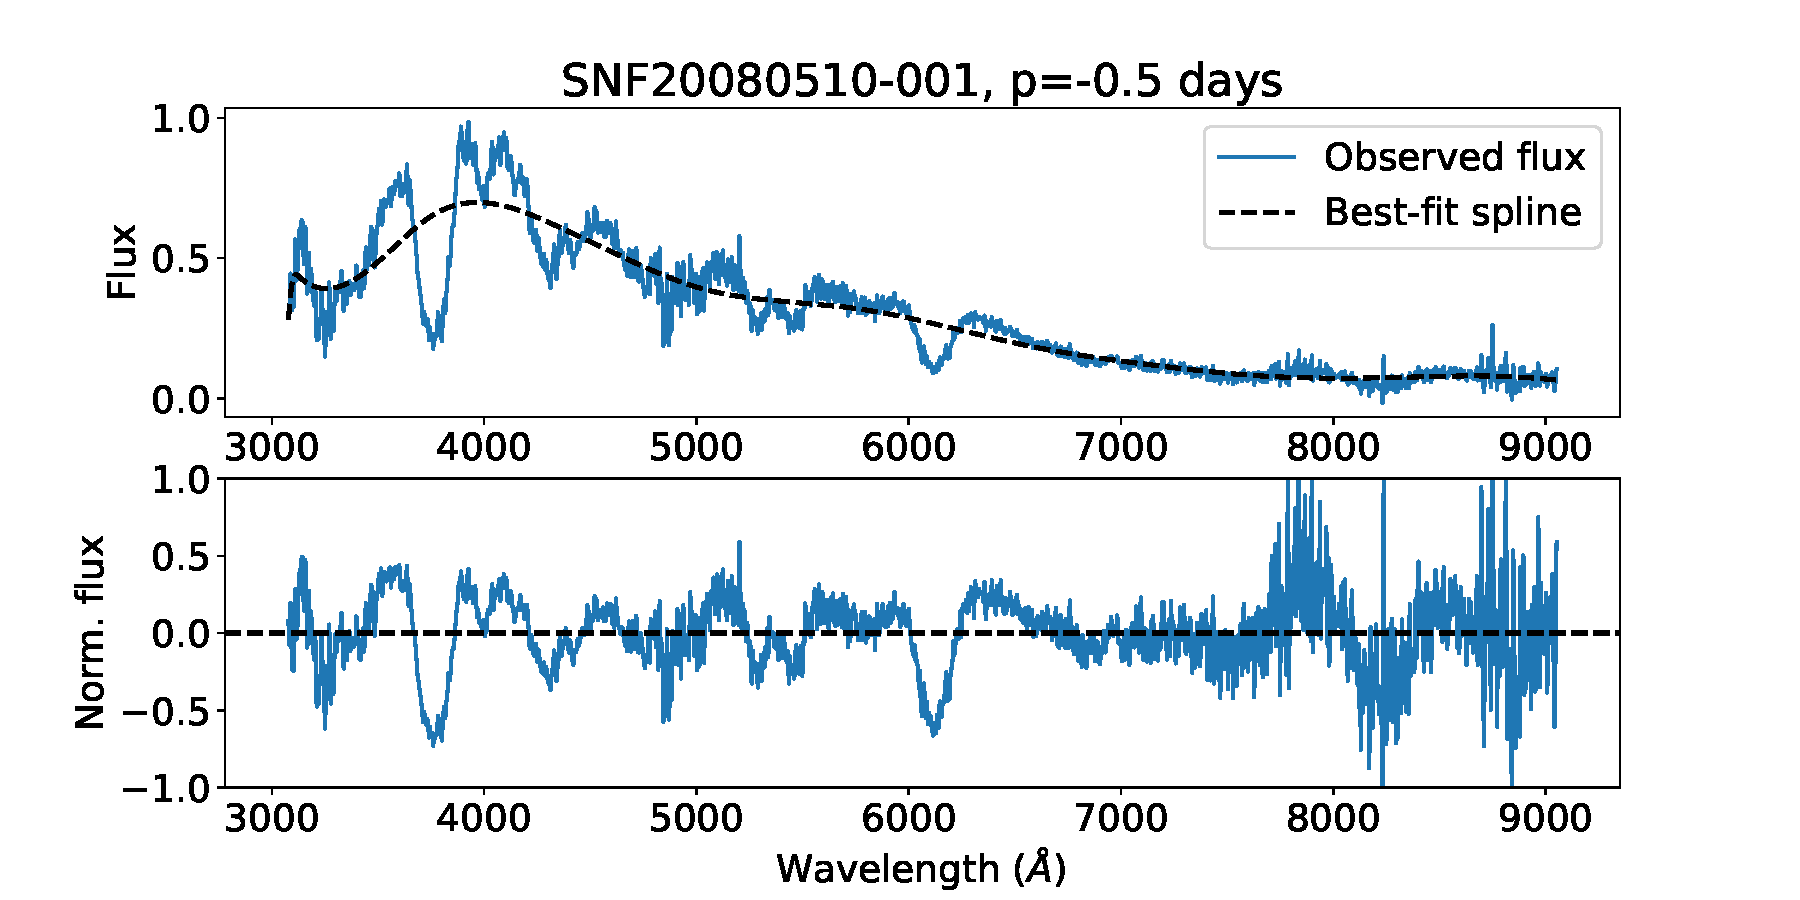
\includegraphics[width=0.9\textwidth]{figures/si_feat_pca/spline_norm_ex.pdf}
    \caption{An example of the preprocessing steps taken to normalize the spectra using a 13-point spline. The upper figure shows the full near-max spectrum along with the best fit spline. The lower figure shows that same spectrum with the spline pseudo-continuum removed.}
    \label{spline_norm_ex}
\end{figure}

\begin{figure}[htbp]
    \centering
    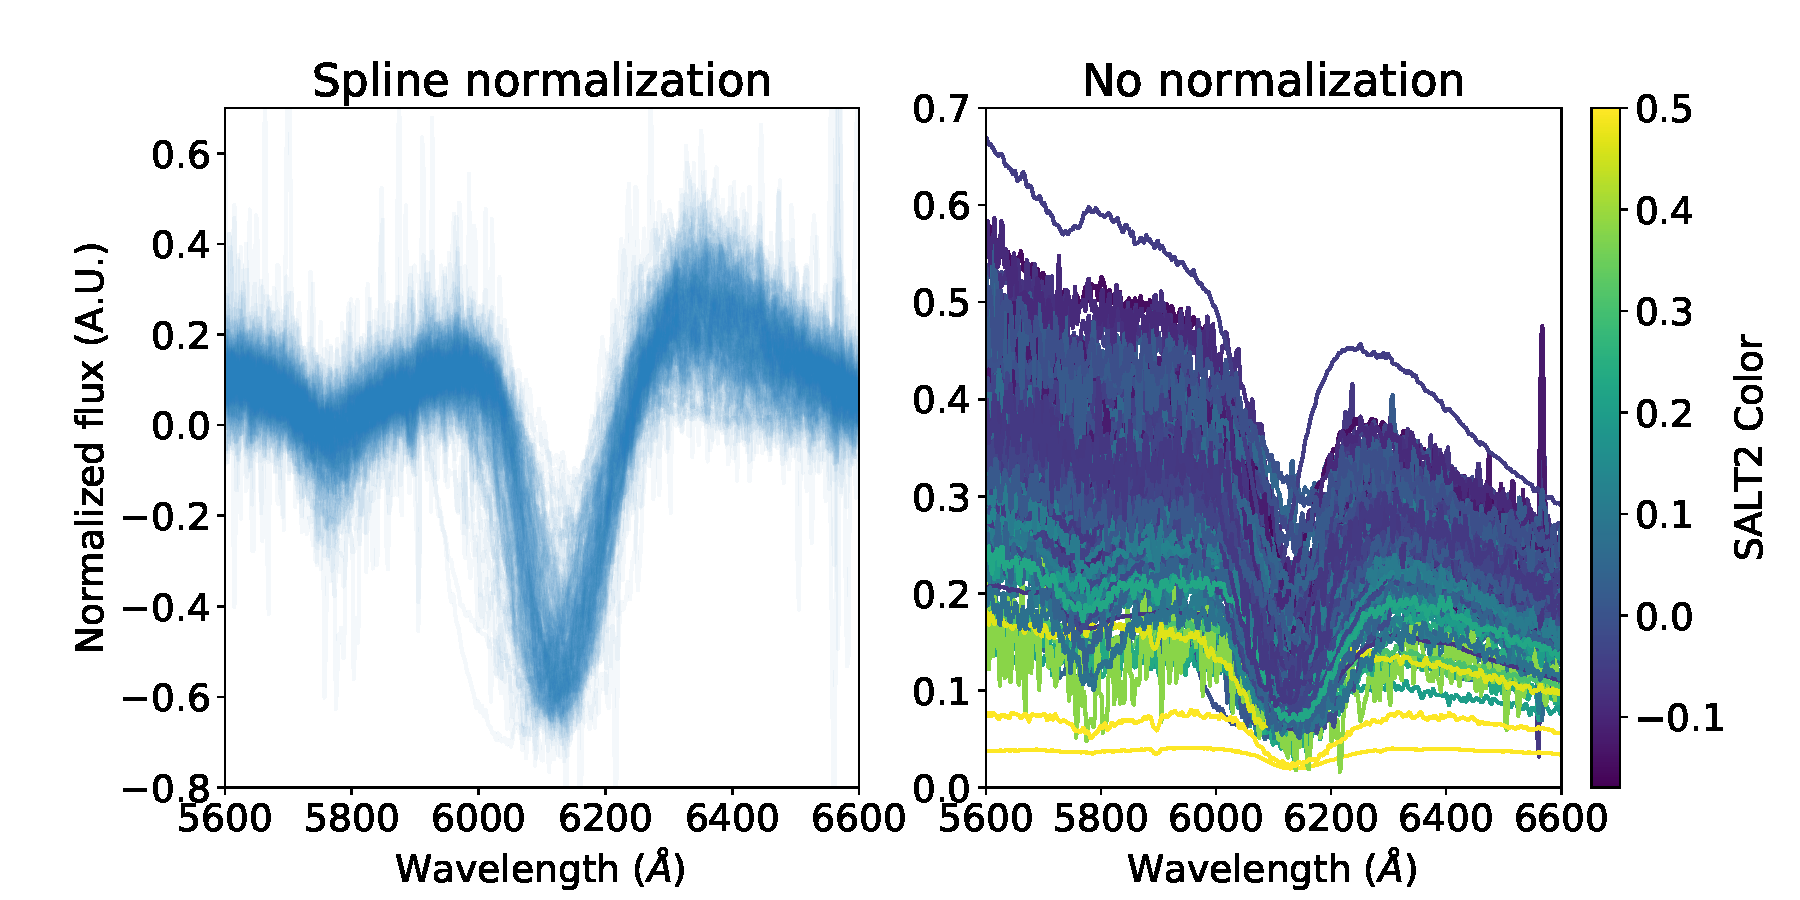
\includegraphics[width=0.9\textwidth]{figures/si_feat_pca/compare_spline_norm.pdf}
    \caption{Zoom-in on the feature of interest for this work, with and without the spline normalization. The features plotted in the right figure are colored by the objects' SALT2 color to emphasize that the effect of this spline normalization is to remove the effects of color on the shape of the spectral feature.}
    \label{compare_spline_norm}
\end{figure}

We also want to ensure that our model generalizes to unseen supernovae by evaluating its performance on an separate test set. This external validation set was taken from the Berkeley Supernova Ia Program \citep[BSNIP,][]{silverman_berkeley_2012}. From the 1298 spectra from 582 objects in this sample, we selected objects with a spectrum within $\pm$3.5 days of maximum brightness and exclude peculiar objects (i.e. those determined to be SN1991T- or SN1999bg-like by SNID). Once again, if one object has more than one spectrum within the phase range allowed, we select the spectrum closest to maximum brightness. This leaves us with a set of 88 spectra. We performed the same preprocessing to these spectra as we did the SNfactory sample spectra. The preprocessed line profiles are also available in the released code repository.

\section{Spectral Feature Measurement}
\label{spectral_features}
As photons from radioactive activity in the inner layers of the supernova explosion make their way through the outer ejecta, they are absorbed by the outer material. This absorption results in the characteristic features in the supernova spectrum. The shape of these absorption lines is governed by myriad physical factors, including the velocity, temperature and density of the ejecta and the optical depth of the various layers of the explosion.

Supernova spectral features profiles are usually quantified using measures of their width and depth, along with their location in the spectrum. The width and depth of the line are summarized by the equivalent width: the width of a rectangle with a height determined by the flux of the continuum such that the area of the rectangle equals the area of the line flux under the continuum. Mathematically, this is
\begin{equation}
    pEW = \displaystyle\int_{\lambda_b}^{\lambda_r}
    \left(1-\frac{f(\lambda)}{f_c(\lambda)}\right)d\lambda,
    \label{equiv_width_eq}
\end{equation}
where $\lambda_b$ and $\lambda_r$ are the wavelength limits of the feature one the blue and red sides, respectively, $f(\lambda)$ is the true flux of the object and $f_c(\lambda)$ is the flux of the continuum.

Calculating the continuum in supernova spectra is challenging, since the absorption features are actually blends of multiple wide lines. Instead, we define a pseudo-continuum by the line connecting the maximum flux values in predefined windows on either side of the absorption feature (see Figure \ref{smooth_example}). These windows are defined in Table \ref{wavelength_ranges}. Throughout the rest of this work, we will use the pseudo-equivalent width, i.e. where $f_c$ in Eq. \ref{equiv_width_eq} is the pseudo-continuum.

\begin{table}[htbp]
    \centering
    \begin{tabular}{cc}\toprule
         Parameter name & Value \\\midrule
         $\lambda_0$ & 6355 \\
         $\lambda_{min}$ & 5600 \\
         $\lambda_{max}$ & 6600 \\
         $\lambda_b$ & 5850-6015 \\
         $\lambda_r$ & 6250-6365 \\\bottomrule
    \end{tabular}
    \caption{Important wavelengths for measuring indicators of the \siliconii{} feature. $\lambda_b$ and $\lambda_r$ are the blue and red windows used when defining the pseudo-continuum.}
    \label{wavelength_ranges}
\end{table}

We can also learn about the ejecta velocities from the location of the absorption feature. We measure the wavelength of maximum absorption $\lambda$ and calculate the velocity using the relativistic Doppler formula:
\begin{equation}
v = c\left[\frac{(\lambda/\lambda_0)^2 -1}{(\lambda/\lambda_0)^2 +1}\right]
\label{doppler}
\end{equation}
where $c$ is the speed of light and $\lambda_0$ is the emission wavelength of the feature (Table \ref{wavelength_ranges}). Because this line is always blue-shifted (the visible ejecta in the line of sight are moving toward the observer), we neglect the minus sign and refer to lines that are more blue-shifted as representing higher velocity ejecta.

\subsection{Baseline: Savitsky-Golay Smoothing}
We begin by establishing a ground truth measurement of the velocities and equivalent widths of all of the supernovae in our training and validation sets. We start by smoothing the spectrum with a Savitsky-Golay filter. The window for this filter is determined optimally as described in Appendix \ref{sg_optimal}. An example smoothed spectrum is shown in Figure \ref{smooth_example}.

Using this smoothed spectrum, we search for the wavelength of maximal absorption (minimum flux) within the window defined by the reddest edge of the blue pseudo-continuum window and the bluest edge of the red pseudo-continuum window and use this wavelength in Eq. \ref{doppler}. We also use the smoothed spectrum to calculate the pseudo-equivalent width with \ref{equiv_width_eq}, where the integration is done with a Riemann sum of the smoothed flux. We estimate our uncertainty on both these measurements using Monte Carlo simulations, repeating the process for spectra with different realizations of the noise. Figure \ref{indicator_scatter_hist} shows the distribution of velocities measured with this technique for all of the supernovae in our training set, and Table \ref{snf_data_table} contains all the velocity and pseudo-equivalent width measurements, along with their uncertainties. Our training set has a mean velocity of $11.0 \times 10^3$~km/s, with a standard deviation of $1.0 \times 10^3$~km/s. 16.5\% of the objects in the sample are high-velocity (defined as in \cite{wang_evidence_2013} as supernovae with $v_{Si}>12000$~km/s). The distribution pseudo-equivalent widths has a mean of 101~\AA{} and standard deviation of 26.2~\AA{}.

\begin{figure}[htbp]
    \centering
    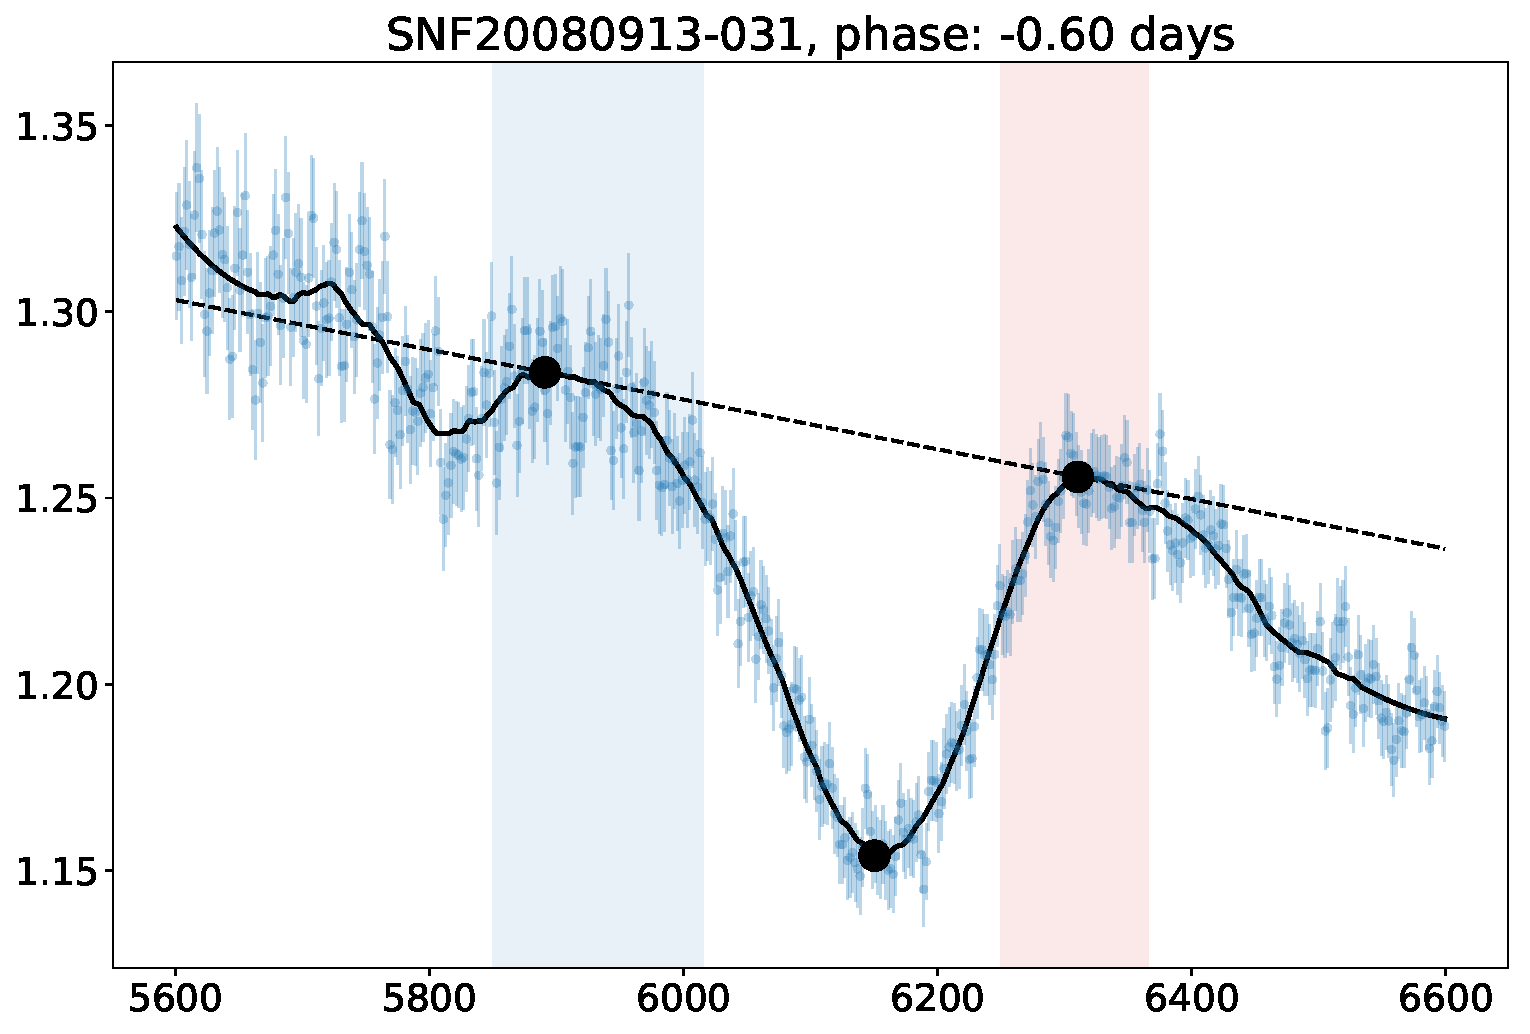
\includegraphics[width=0.9\textwidth]{figures/si_feat_pca/example_measure.pdf}
    \caption{An example \siliconii{} feature. The original data is shown in blue along with the uncertainties. The optimal smoothing is shown in the thick black line. The blue and red spans show the location of the wavelength windows used to search for the maxima defining the pseudo-continuum (the maxima are the large black points). The pseudo-continuum is plotted as the dashed black line. The location of the maximum absorption wavelength is also shown as a large black point.}
    \label{smooth_example}
\end{figure}

\begin{figure}[htbp]
    \centering
    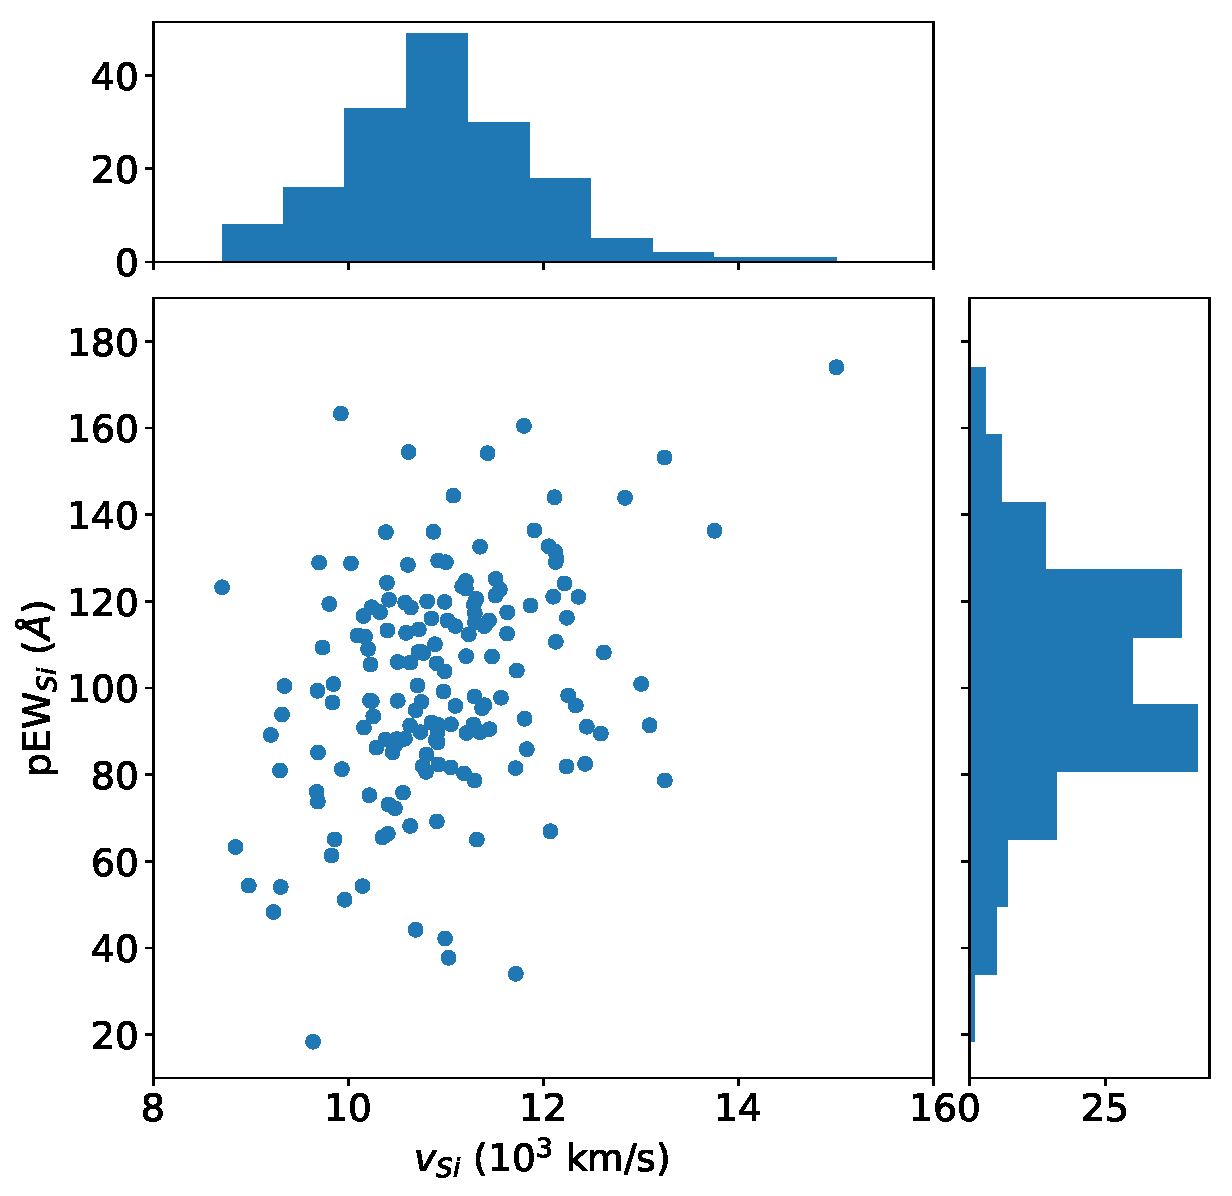
\includegraphics[width=0.9\textwidth]{figures/si_feat_pca/spectral_features_training_scatter_hist.pdf}
    \caption{Distributions of the spectral indicators of the \siliconii{} feature from the training set.}
    \label{indicator_scatter_hist}
\end{figure}

\begin{longtable}{ccccc}
\caption{The baseline spectral feature data used throughout this analysis for both the training Nearby Supernova Factory data and the validation BSNIP sample.} \label{snf_data_table}\\
\toprule
Name & $v_{Si}$ (km/s) & $\Delta$ $v_{Si}$ (km/s) & pEW (\AA) & $\Delta$ pEW (\AA) \\
\midrule
\endfirsthead
\multicolumn{4}{c}{Continued}\\
\toprule
Name & $v_{Si}$ (km/s) & $\Delta$ $v_{Si}$ (km/s) & pEW (\AA) & $\Delta$ pEW (\AA) \\
\midrule
\endhead
\midrule
\multicolumn{4}{c}{Table continues}\\
\midrule
\endfoot
\bottomrule
\endlastfoot
SNF20060911-014 & 11301 & 266 & 78.6 & 6.1 \\
PTF11bnx & 10225 & 591 & 125.2 & 5.5 \\
PTF09dnl & 12300 & 50 & 92.5 & 2.2 \\
PTF09dnp & 13176 & 27 & 92.5 & 2.8 \\
SNF20080514-002 & 11038 & 250 & 95.9 & 2.0 \\
SNBOSS38 & 10789 & 315 & 81.2 & 0.7 \\
SN2006ob & 11221 & 795 & 134.9 & 5.6 \\
SNF20070817-003 & 10875 & 839 & 134.9 & 5.9 \\
SNNGC4424 & 10424 & 57 & 73.2 & 1.2 \\
PTF10qyz & 11054 & 397 & 155.5 & 4.9 \\
LSQ12fxd & 11043 & 331 & 80.5 & 2.5 \\
% SNF20080821-000 & 11409 & 296 & 99.5 & 8.0 \\
% SN2010dt & 10667 & 391 & 124.8 & 3.3 \\
% SNF20080623-001 & 11085 & 236 & 110.1 & 4.6 \\
% LSQ12fhe & 11665 & 302 & 37.0 & 2.5 \\
% PTF11mty & 9770 & 478 & 122.5 & 10.6 \\
% SNF20080512-010 & 11523 & 549 & 122.6 & 6.6 \\
% PTF10tce & 12690 & 236 & 110.8 & 2.6 \\
% SN2005ir & 13804 & 197 & 150.6 & 7.0 \\
% PTF10nlg & 11416 & 565 & 165.1 & 4.4 \\
% PTF10hmv & 9604 & 282 & 75.5 & 3.4 \\
% SNF20071015-000 & 10786 & 73 & 101.1 & 3.5 \\
% SNhunt89 & 11966 & 792 & 144.6 & 4.9 \\
% SNF20080707-012 & 12467 & 520 & 166.0 & 9.3 \\
% PTF09dlc & 10428 & 437 & 99.4 & 6.4 \\
% SN2012cu & 10573 & 309 & 75.5 & 0.6 \\
% SNF20080919-000 & 10193 & 391 & 98.3 & 4.3 \\
% SNF20080919-001 & 9970 & 395 & 58.1 & 3.7 \\
% SN2010kg & 13201 & 129 & 154.2 & 1.1 \\
% SNF20080714-008 & 11752 & 1260 & 168.4 & 8.0 \\
% SNF20061111-002 & 10410 & 159 & 133.6 & 5.2 \\
% SNNGC6343 & 10980 & 266 & 114.1 & 2.5 \\
% PTF10wof & 12078 & 311 & 134.9 & 3.0 \\
% PTF10ufj & 10792 & 280 & 120.5 & 6.4 \\
% CSS130502_01 & 11022 & 52 & 102.0 & 3.4 \\
% SNF20080626-002 & 11629 & 194 & 83.1 & 1.9 \\
% SNF20060621-015 & 10488 & 527 & 98.0 & 2.7 \\
% SNF20070701-005 & 9612 & 295 & 86.4 & 6.0 \\
% SNF20080909-030 & 8925 & 154 & 69.7 & 3.4 \\
% SNNGC2691 & 11140 & 127 & 37.8 & 1.8 \\
% PTF13asv & 9848 & 354 & 55.0 & 2.7 \\
% CSS110918_01 & 12195 & 128 & 83.2 & 2.5 \\
% CSS110918_02 & 10659 & 308 & 107.4 & 3.3 \\
% SNF20080918-002 & 10719 & 309 & 117.3 & 6.8 \\
% SNIC3573 & 10833 & 570 & 110.7 & 5.1 \\
% SNF20080918-000 & 11845 & 440 & 103.7 & 5.9 \\
% SNF20060512-002 & 12749 & 259 & 107.5 & 3.7 \\
% PTF12iiq & 14955 & 266 & 176.7 & 1.7 \\
% SNF20070725-001 & 10157 & 553 & 93.8 & 5.8 \\
% SNF20070902-018 & 11237 & 715 & 146.4 & 9.3 \\
% LSQ12gxj & 11777 & 532 & 97.6 & 4.6 \\
% SN2006cj & 10964 & 377 & 90.8 & 4.2 \\
% SNF20080815-017 & 11149 & 751 & 142.9 & 12.2 \\
% PTF10icb & 10325 & 198 & 87.2 & 0.9 \\
% SNF20061022-005 & 9576 & 311 & 76.8 & 6.9 \\
% PTF13azs & 10647 & 650 & 128.1 & 7.5 \\
% SNF20080612-003 & 11484 & 167 & 83.4 & 3.6 \\
% SNF20070820-000 & 9859 & 509 & 127.3 & 6.5 \\
% SNF20071108-021 & 9101 & 582 & 74.3 & 8.4 \\
% PTF12evo & 10068 & 535 & 106.4 & 8.4 \\
% SNF20050624-000 & 10393 & 679 & 104.7 & 8.8 \\
% SNF20080531-000 & 11386 & 334 & 119.9 & 3.4 \\
% PTF12ikt & 10155 & 442 & 101.8 & 3.9 \\
% PTF12eer & 10418 & 687 & 175.5 & 13.0 \\
% SN2005hj & 10542 & 600 & 72.6 & 4.7 \\
% SNPGC51271 & 11264 & 173 & 113.5 & 4.1 \\
% SNPGC027923 & 10930 & 255 & 69.7 & 2.2 \\
% SNF20080522-011 & 10929 & 223 & 98.2 & 4.2 \\
% SNhunt46 & 10975 & 236 & 91.7 & 1.8 \\
% SNF20071021-000 & 11636 & 297 & 123.6 & 1.7 \\
% SNF20070831-015 & 10421 & 467 & 93.5 & 5.5 \\
% SNF20080806-002 & 10666 & 324 & 99.4 & 4.1 \\
% SNF20080822-005 & 10553 & 311 & 76.4 & 5.8 \\
% PTF10zdk & 9766 & 316 & 106.9 & 2.7 \\
% SNF20070424-003 & 10957 & 425 & 122.0 & 6.6 \\
% SNF20070714-007 & 9446 & 533 & 129.3 & 2.9 \\
% PTF11cao & 12017 & 518 & 144.5 & 2.5 \\
% SNF20061021-003 & 10932 & 445 & 115.0 & 4.6 \\
% PTF11pdk & 10379 & 265 & 129.8 & 8.2 \\
% SNF20070506-006 & 9734 & 229 & 67.3 & 3.8 \\
% SN2005hc & 11117 & 458 & 102.8 & 4.0 \\
% SN2007bd & 12412 & 472 & 125.4 & 2.4 \\
% PTF10wnm & 11452 & 227 & 102.1 & 5.6 \\
% SN2010ex & 10598 & 452 & 85.0 & 3.8 \\
% SNF20080802-006 & 11827 & 933 & 139.0 & 9.7 \\
% PTF10xyt & 12134 & 141 & 129.2 & 6.9 \\
% SNF20070727-016 & 10518 & 127 & 72.4 & 4.6 \\
% SNF20070818-001 & 12023 & 668 & 158.2 & 11.9 \\
% SNF20070427-001 & 10330 & 491 & 87.2 & 7.0 \\
% PTF10ops & 9617 & 1520 & 207.9 & 20.9 \\
% SNF20080614-010 & 10635 & 418 & 145.7 & 6.4 \\
% PTF10ndc & 11145 & 192 & 102.0 & 6.4 \\
% SNF20080323-009 & 9902 & 246 & 107.7 & 8.4 \\
% SNF20080516-022 & 9136 & 278 & 106.6 & 4.3 \\
% SNF20070802-000 & 11799 & 674 & 145.1 & 8.9 \\
% SN2004gs & 11180 & 45 & 137.0 & 1.5 \\
% SNF20050824-002 & 11286 & 1034 & 133.9 & 13.1 \\
% PTF10mwb & 10816 & 313 & 117.5 & 1.9 \\
% PTF09foz & 10183 & 220 & 115.7 & 2.4 \\
% PTF09fox & 11345 & 603 & 109.8 & 3.8 \\
% SNF20061030-010 & 11365 & 172 & 114.3 & 2.6 \\
% SNF20061020-000 & 11406 & 422 & 119.0 & 3.3 \\
% PTF12ena & 10758 & 334 & 86.8 & 2.1 \\
% PTF13anh & 8674 & 485 & 133.2 & 4.9 \\
% SNF20080725-004 & 11216 & 109 & 110.1 & 6.9 \\
% SNF20070403-001 & 11055 & 596 & 139.3 & 10.5 \\
% LSQ12dbr & 10486 & 116 & 72.3 & 3.1 \\
% SNF20070902-021 & 10452 & 685 & 123.1 & 5.8 \\
% PTF11mkx & 9592 & 529 & 56.0 & 6.8 \\
% SNF20060907-000 & 10176 & 237 & 117.1 & 2.9 \\
% SNF20080717-000 & 12735 & 408 & 99.9 & 5.4 \\
% SNF20080825-010 & 11233 & 616 & 127.9 & 3.6 \\
% SNF20070717-003 & 9812 & 876 & 149.6 & 6.9 \\
% SN2004ef & 11924 & 502 & 134.8 & 2.2 \\
% SNNGC7589 & 13249 & 138 & 81.1 & 2.6 \\
% SNF20080516-000 & 10809 & 627 & 101.7 & 8.5 \\
% SNF20080620-000 & 10876 & 546 & 127.2 & 3.6 \\
% SNF20050728-006 & 11324 & 407 & 128.5 & 6.7 \\
% SNF20050821-007 & 10567 & 332 & 96.3 & 5.0 \\
% SNF20080920-000 & 12995 & 432 & 109.0 & 4.7 \\
% SNF20080918-004 & 10161 & 430 & 124.7 & 4.5 \\
% SN2012fr & 12085 & 36 & 67.2 & 0.7 \\
% SNF20080610-000 & 10739 & 341 & 129.9 & 6.5 \\
% SNF20060512-001 & 8890 & 295 & 58.2 & 4.7 \\
% SN2007kk & 11833 & 407 & 117.9 & 5.1 \\
% PTF11bgv & 9681 & 218 & 99.9 & 3.2 \\
% SNF20070806-026 & 11418 & 744 & 126.5 & 3.2 \\
% PTF11kly & 10502 & 89 & 97.3 & 0.3 \\
% SNF20060912-000 & 9392 & 309 & 104.2 & 7.5 \\
% SNF20071003-016 & 11002 & 824 & 133.7 & 6.4 \\
% SNF20070803-005 & 9719 & 252 & 25.4 & 4.0 \\
% PTF12fuu & 10872 & 502 & 96.3 & 6.7 \\
% SN2007nq & 11954 & 490 & 127.2 & 3.2 \\
% SNF20080810-001 & 10446 & 340 & 111.5 & 2.0 \\
% SN2008ec & 10892 & 170 & 120.8 & 1.0 \\
% SNF20060618-014 & 11717 & 754 & 123.3 & 6.9 \\
% SNNGC2370 & 10878 & 121 & 120.5 & 2.4 \\
% SNF20070403-000 & 9413 & 663 & 122.7 & 7.6 \\
% SNNGC4076 & 9488 & 432 & 81.8 & 2.5 \\
% SNF20070630-006 & 11130 & 321 & 124.8 & 12.0 \\
% SNF20061108-004 & 11839 & 404 & 129.2 & 9.1 \\
% SNF20080914-001 & 9290 & 301 & 93.2 & 2.5 \\
% SNF20060609-002 & 10734 & 497 & 89.9 & 3.9 \\
% SN2006do & 12363 & 153 & 120.4 & 2.4 \\
% SN2006dm & 11280 & 363 & 121.1 & 1.1 \\
% SNF20060526-003 & 11200 & 385 & 100.7 & 5.5 \\
% PTF10qjq & 10884 & 24 & 92.1 & 2.4 \\
% SNF20080507-000 & 10752 & 268 & 98.6 & 7.0 \\
% SNF20070330-024 & 12422 & 56 & 85.5 & 3.6 \\
% PTF11bju & 10683 & 260 & 45.3 & 3.9 \\
% SNF20060521-001 & 10712 & 482 & 119.6 & 5.4 \\
% PTF11drz & 11295 & 434 & 129.0 & 4.4 \\
% SNNGC0927 & 11726 & 288 & 106.8 & 2.5 \\
% PTF12dxm & 10654 & 823 & 146.1 & 6.7 \\
% SNF20080803-000 & 11231 & 475 & 112.0 & 7.1 \\
% SNF20060511-014 & 10345 & 289 & 132.0 & 5.1 \\
% PTF12ghy & 10657 & 586 & 107.7 & 2.8 \\
% SNF20070531-011 & 11694 & 588 & 130.4 & 2.8 \\
% SNF20080522-000 & 11054 & 553 & 52.0 & 4.8 \\
% SNF20080510-005 & 11391 & 566 & 104.0 & 8.6 \\
% SNF20070712-003 & 9892 & 608 & 110.6 & 5.5 \\
% SNF20080913-031 & 10075 & 728 & 93.9 & 7.8 \\
% SNF20080510-001 & 11347 & 438 & 133.5 & 6.3 \\
\end{longtable}


This technique for smoothing the spectrum works very well when the spectrum has reasonable resolution and a high signal-to-noise ratio. However, as the resolution and signal-to-noise level decreases, so too does our ability to recover both the limits of the pseudo-continuum and the true location of maximum absorption. 

\subsection{Gaussian Absorption Line Model}
One way to work around the limitations of low resolution spectroscopy would be to assume some functional form for the absorption feature being studied. A common -- though not very descriptive -- choice is a Gaussian. Using such an inflexible function to capture the line information biases the results. To illustrate this, we fit the same data with a model assuming a linear continuum in the wavelength range of interests along with a Gaussian absorption line. Figure \ref{gauss_feat_fit} shows an example of such a fit. We can see that the full morphology of the feature is not totally captured. More quantitatively, we show in Figure \ref{gauss_bias} a histogram of the difference between the velocity measured from using a Gaussian line profile with a linear continuum and the velocity measured from smoothing and finding the maximum absorption wavelength. There is a clear bias in the velocity; on average, the velocity measured with the Gaussian profile is 200~km/s higher than the true velocity. The pseudo-equivalent width measurements are also slightly biased; on average, the Gaussian measured pEWs are 5~\AA{} narrower than the true values.

\begin{figure}
    \centering
    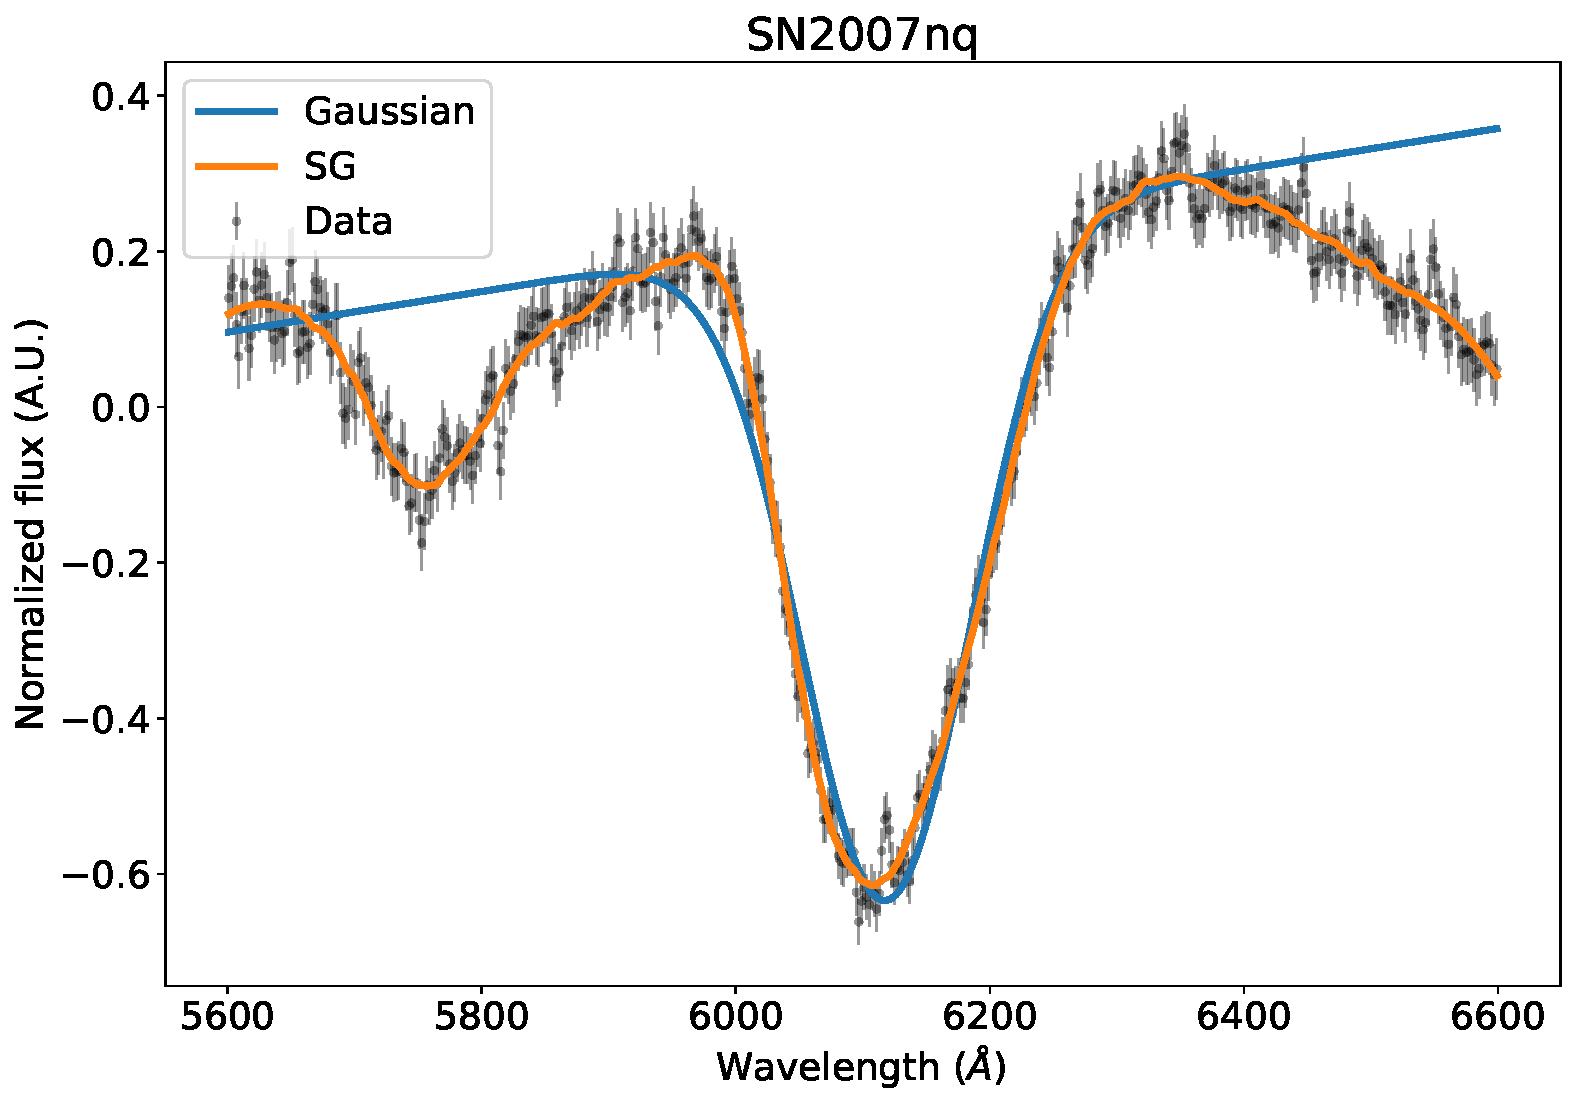
\includegraphics[width=0.9\textwidth]{figures/si_feat_pca/gauss_fit_example.pdf}
    \caption{Comparison of the \siliconii{} feature fit to a Gaussian and the Savitsky-Golay smoothing for SN2007nq. We can see that the blue edge of the feature is not properly captured. The minimum of the feature is also located at different wavelengths, which will produce an inaccurate velocity measurement.}
    \label{gauss_feat_fit}
\end{figure}

\begin{figure}[htbp]
    \centering
    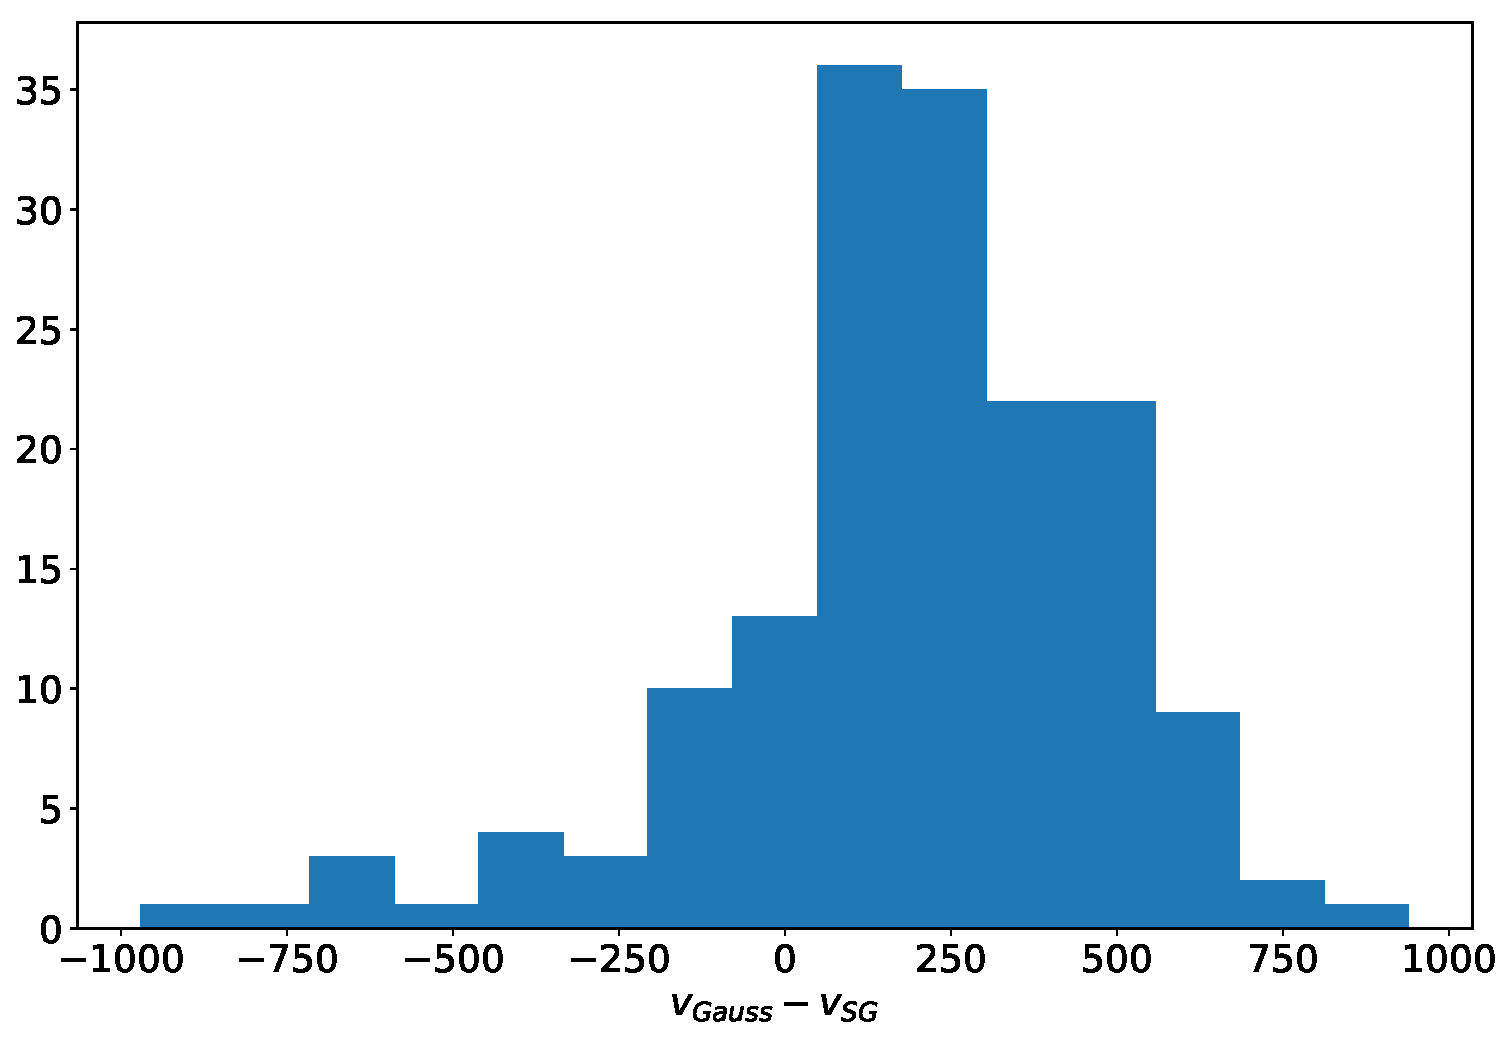
\includegraphics[width=0.9\textwidth]{figures/si_feat_pca/gauss_bias.pdf}
    \caption{Histograms of residuals between the velocity and equivalent width of the \siliconii{} line measured using a Gaussian line profile and the true velocity. There is a clear bias, with the Gaussian measurement giving velocity values that are on average 200~km/s higher than the true values, and equivalent width values that are 5~\AA{} narrower.}
    \label{gauss_bias}
\end{figure}


\section{EMFA of the SiII \texorpdfstring{$\lambda$}{}6355 Feature}
\label{method}
Our goal is to introduce a method of inferring the shape of the \siliconii{} feature that is robust to noise and resolution degradation and also accounts for the true diversity of shapes the spectral feature can take on. We accomplish these goals by performing expectation-maximization factor analysis on the normalized spectral features.

\subsection{Expectation Maximization Factor Analysis}
A common unsupervised learning task is dimensionality reduction: using a data set with many features to find a smaller number of principal features that are sufficient to model the data set. The most commonly used technique for dimensionality reduction is principal component analysis, which linearly maps data to a lower-dimensional subspace of the original feature space in such a way as to maximize the data variance. In this analysis, we use a related dimensionality reduction technique: expectation-maximization factor analysis.

Consider a set of $p$ $n$-dimensional data vectors $\{\bm{y}^1, ..., \bm{y}^p\}$. Now assume that there exists some $k$ unobserved latent variables $\{\bm{x}^1, ..., \bm{x}^k\}$, themselves each $n$-dimensional vectors. Each data vector is then generated by
\begin{equation}
\bm{y} - \bm{\mu} = \bm{\Lambda}\bm{x}+\bm{\epsilon}
\end{equation}
where $\bm{\mu}$ is an $n$-dimensional mean vector and $\bm{\epsilon}$ is a noise vector that is Gaussian distributed with mean 0 and covariance $\bm{\Psi}$. The matrix $\bm{\Lambda}$ is known as the loading matrix and describes the relative contributions of each factor to the observed variables.

This statistical formulation is quite similar to principle component analysis; indeed, the components found with factor analysis are often quite similar to those found using principle component analysis. However, the two techniques differ in their assumptions on the covariance matrix $\bm{\Psi}$. In the PCA framework, $\bm{\Psi}=\sigma^2\bm{I}$, while in EMFA, $\bm{\Psi}$ can be any diagonal matrix. This means that EMFA gives more general description of the noise.

We train the factor loadings using an expectation-maximization (EM) approach. Expectation maximization is an iterative technique for maximizing a likelihood with latent variables. The first step (the E-step) finds the expectation value of the hidden variables given the model parameters. The next step (the M-step) fits the model parameters to maximize the likelihood given the expectation value of the hidden variables. These steps are repeated until convergence.

In our case, each of the observables is the flux in some wavelength bin, and the factors $F_i$ are $n$-dimensional vectors, where $n$ is the number of flux bins in the training spectra. For this analysis, we used the factor analysis implementation included in the \verb|scikit-learn| Python package \citep{pedregosa_scikit-learn_2011}.

\subsection{Visualizing Model Components}
The EMFA components are shown in Figure \ref{emfa_components}. Each figure shows the impact of adding a range of loading factors (elements of the loading matrix $\bm{\Lambda}$) to the mean spectral feature. We qualitatively see how the velocity and equivalent width is affected by each components. Higher loadings of component 1 correspond to higher velocity and larger equivalent width lines. Higher loadings of component 2 correspond to high velocity, but shallower features. The third component modifies the shape of the bluer portion of the feature. Similar effects can be seen in the nearby Si II $\lambda$5972 feature.

\begin{figure}[htbp]
    \centering
    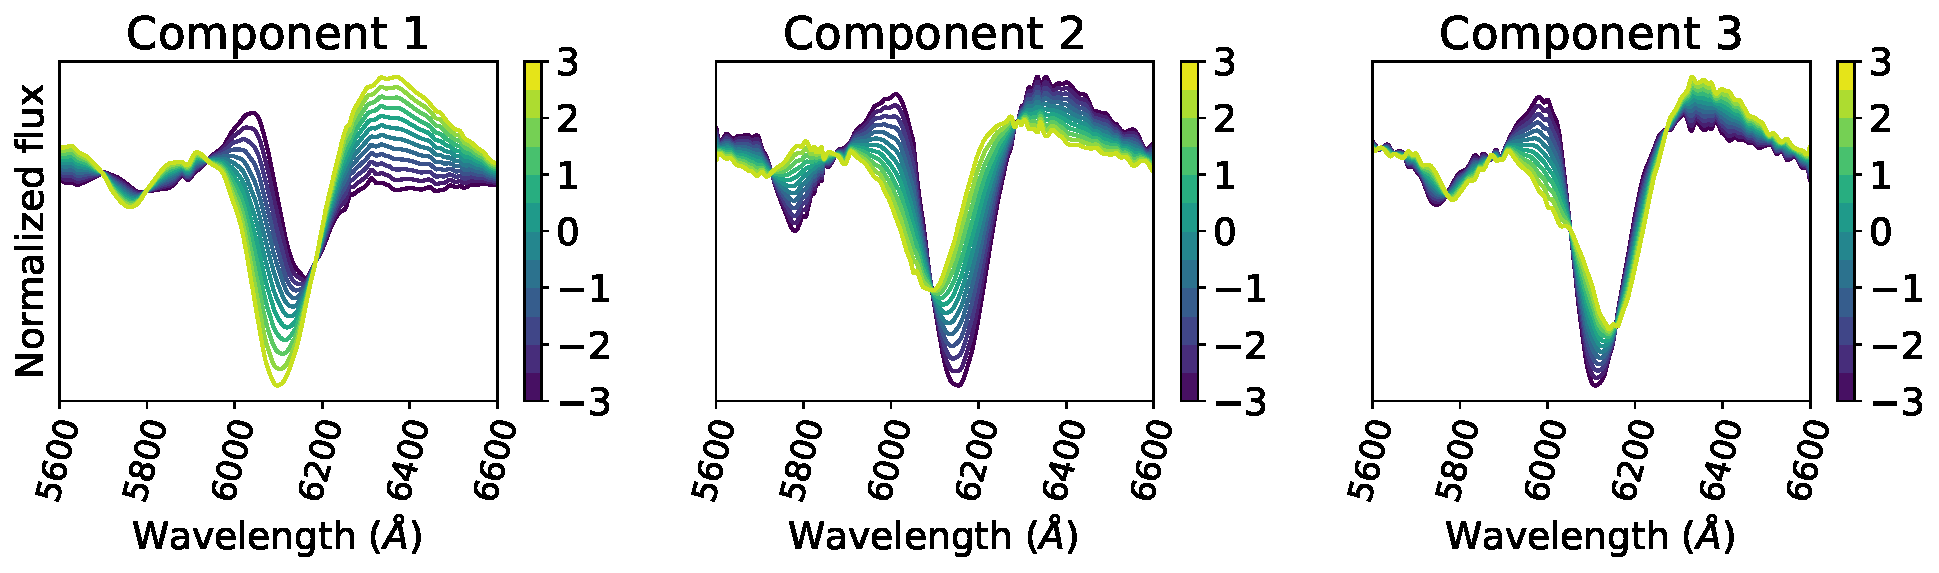
\includegraphics[width=0.9\textwidth]{figures/si_feat_pca/model_components.pdf}
    \caption{Visualization of the components ($\bm{x}$) of the EMFA model. Each subfigure shows the effect of adding various values of multiples of the components to the mean vector.}
    \label{emfa_components}
\end{figure}

The distributions of the loading coefficients are shown in Figure \ref{corner_plot_vel} and \ref{corner_plot_ew}. The qualitative observations about the relationship between the loading coefficients and the velocity and equivalent widths of the feature are confirmed there, as well as in Figure \ref{scatter_loading} where the spectral indicator measurements are plotted directly against the loading coefficients of each object in the training sample.

\begin{figure}[htbp]
    \centering
    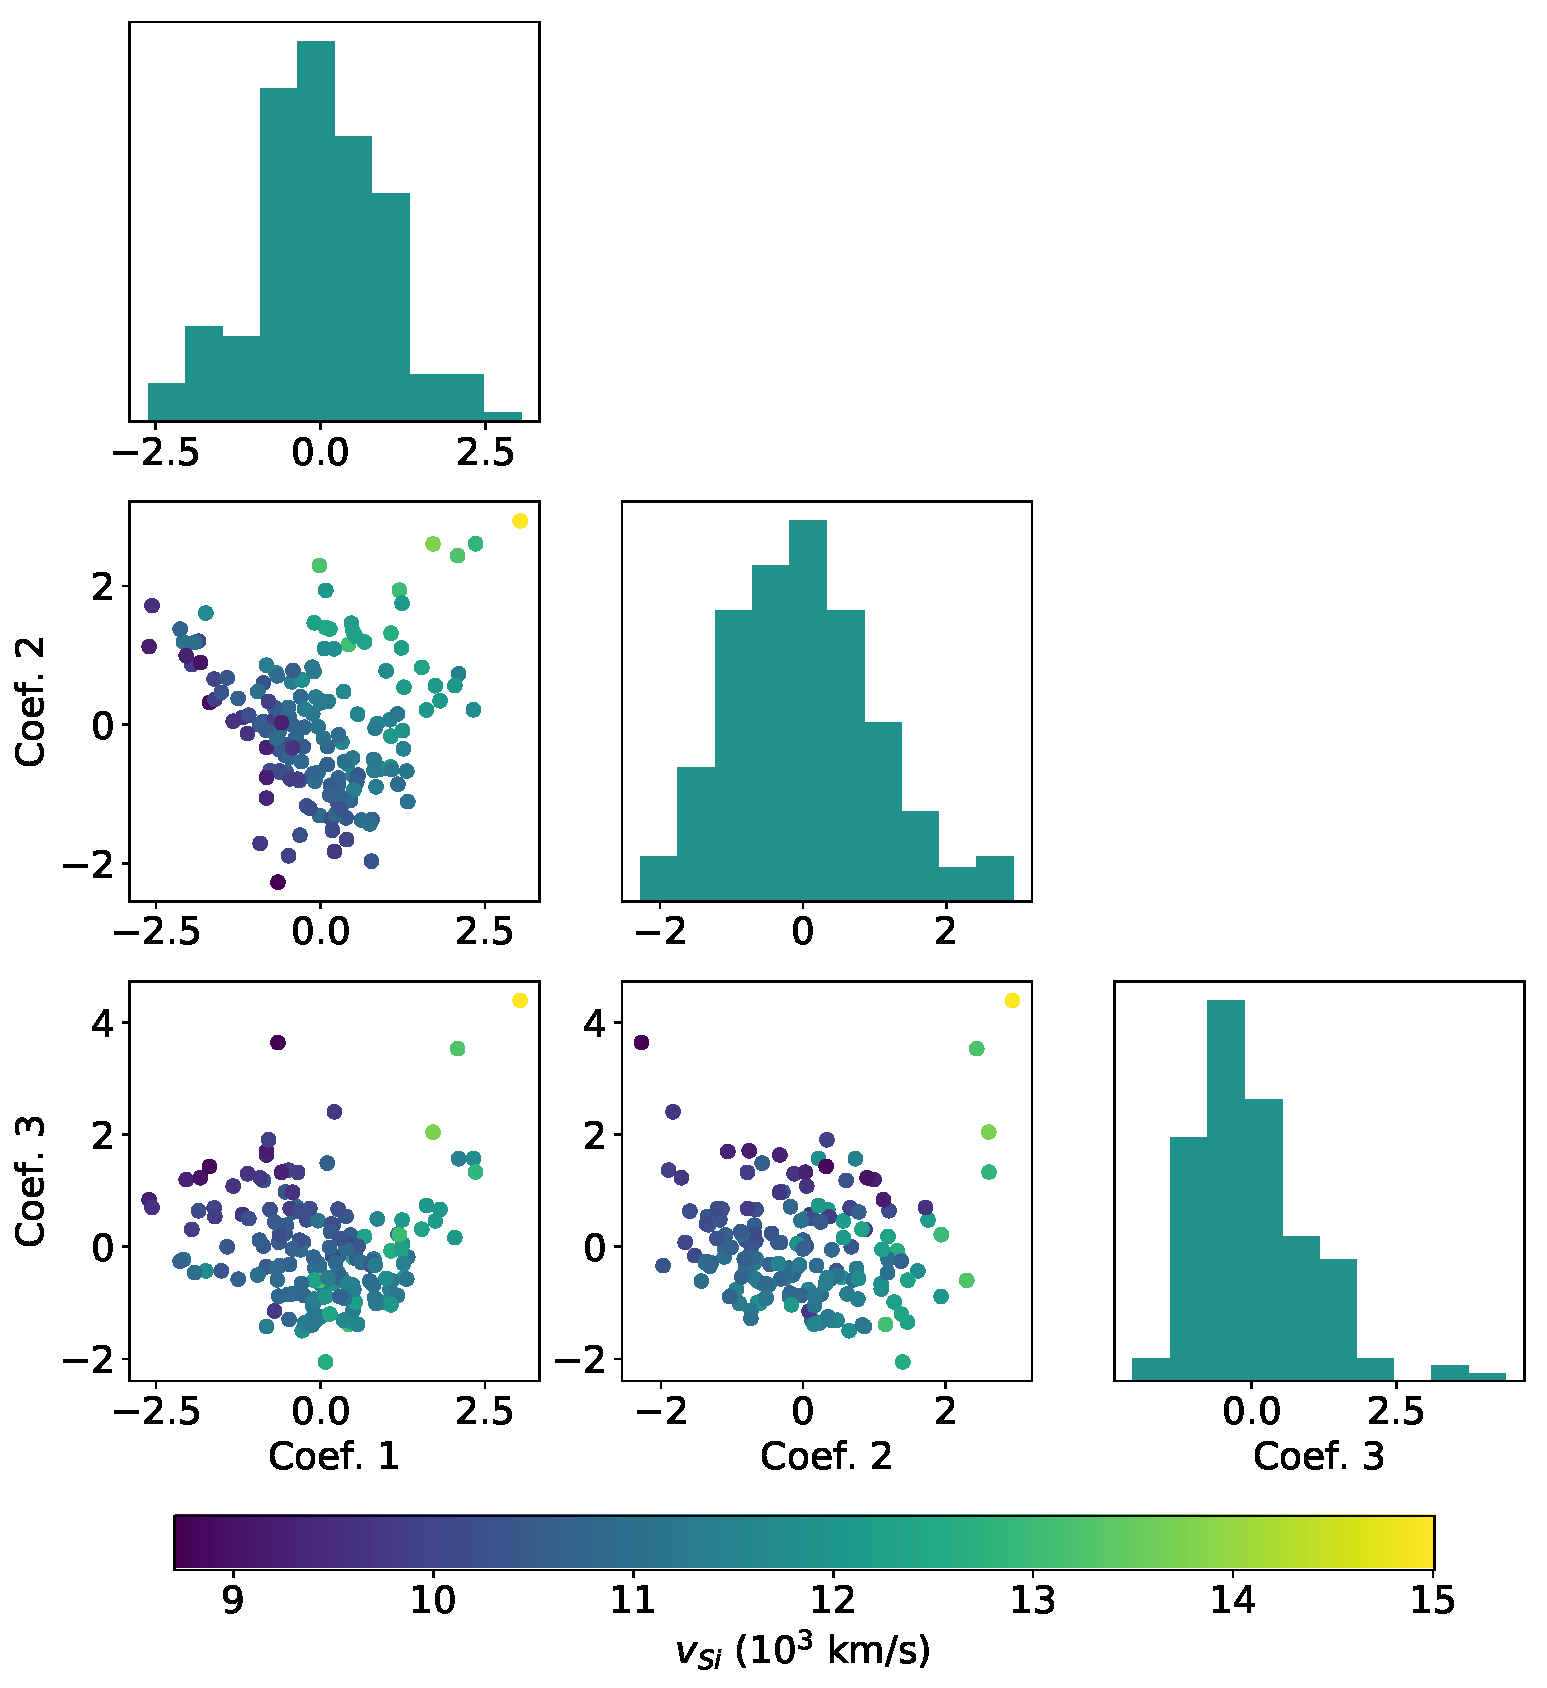
\includegraphics[width=0.9\textwidth]{figures/si_feat_pca/corner_plot_vel.pdf}
    \caption{Corner plot showing the marginal distributions of the loading coefficients for the training set, colored by the measured velocity of the \siliconii{} feature. Each point in the scatter plot represents one supernova.}
    \label{corner_plot_vel}
\end{figure}

\begin{figure}[htbp]
    \centering
    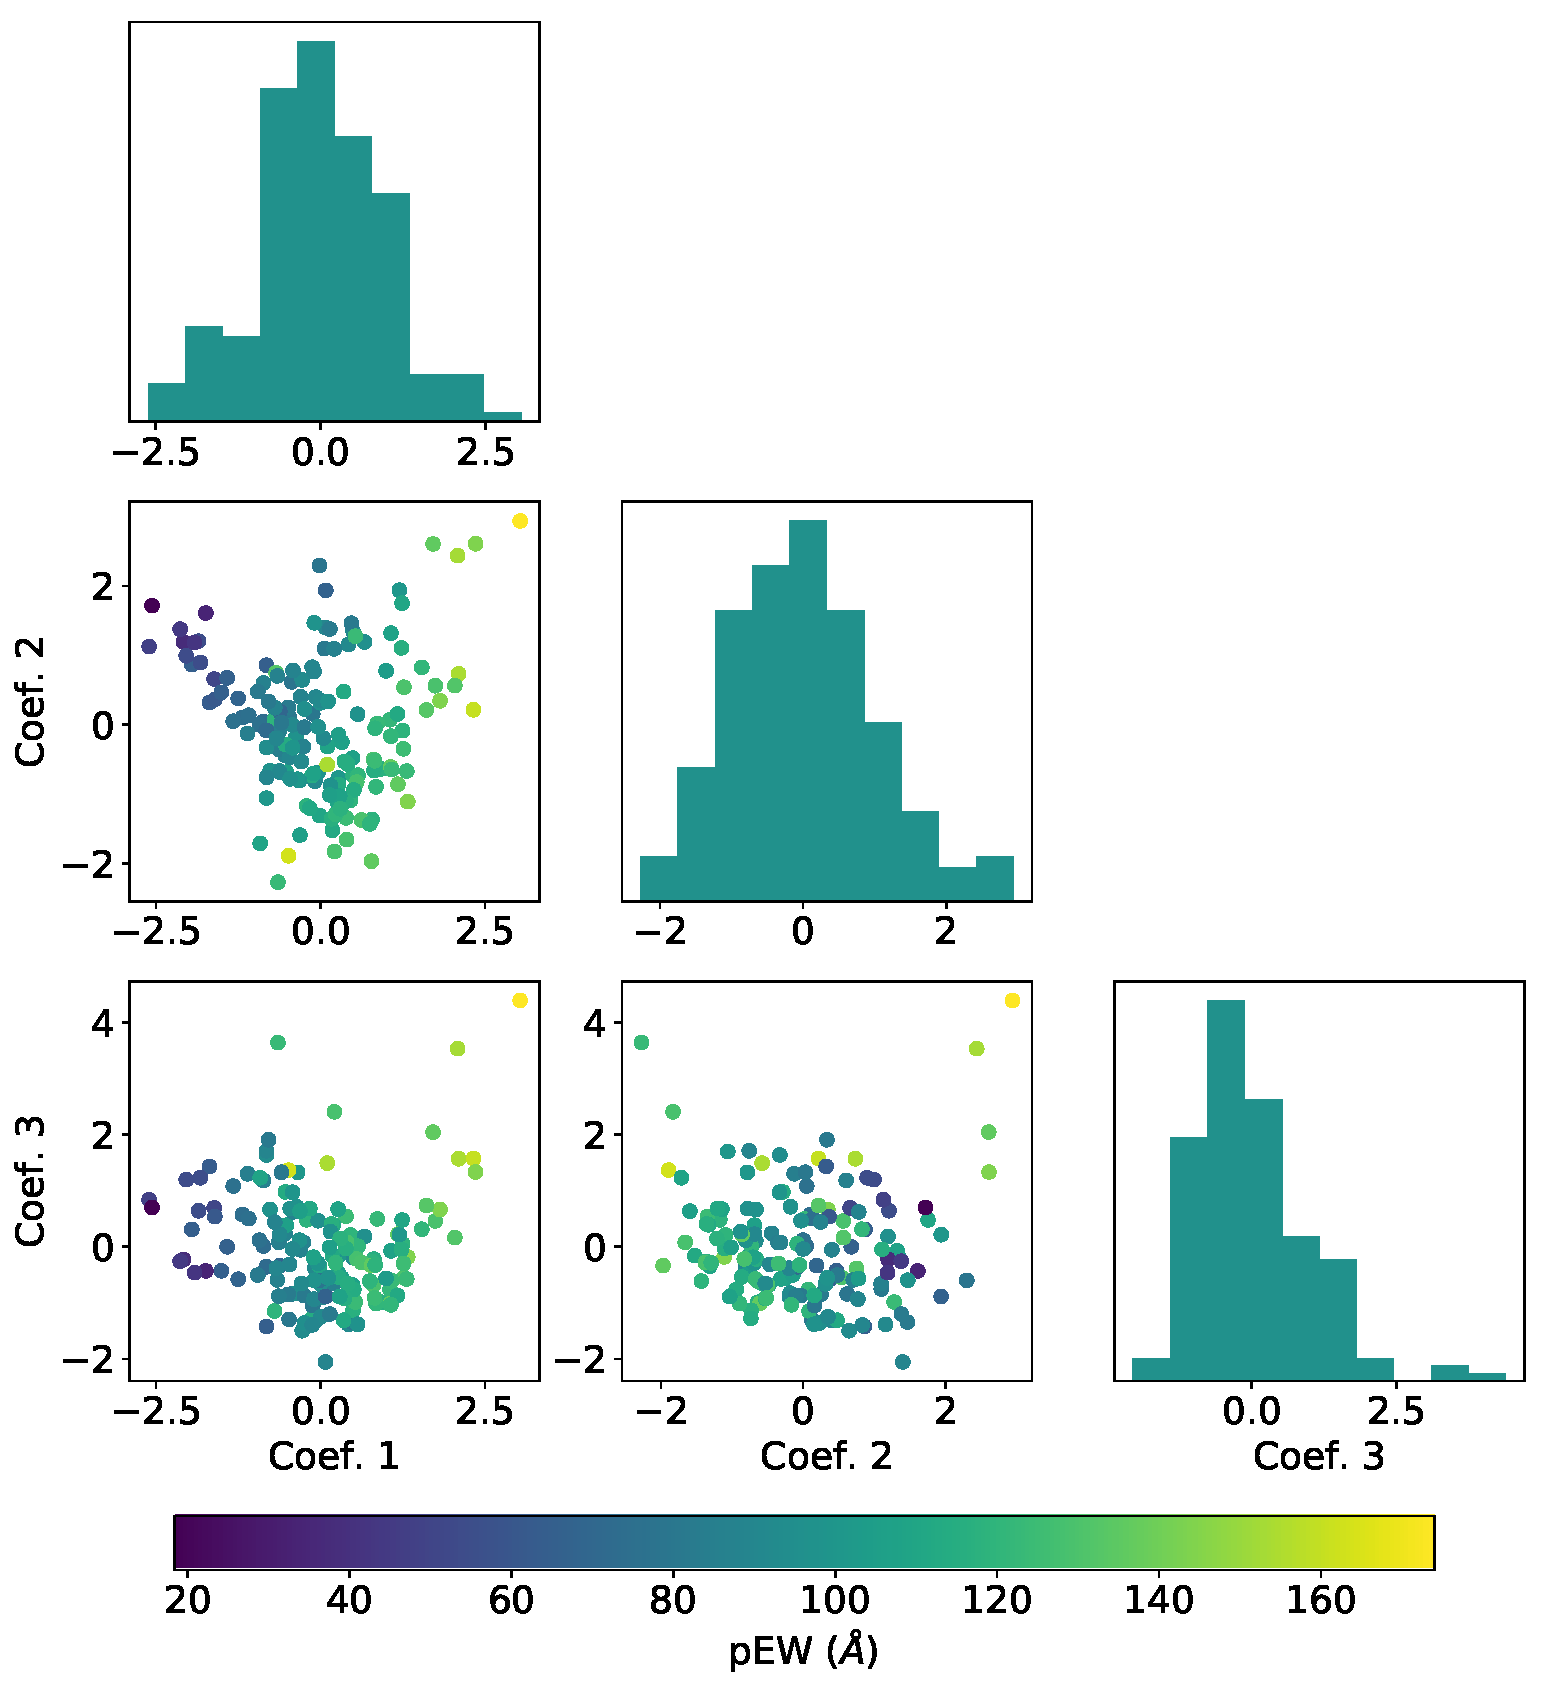
\includegraphics[width=0.9\textwidth]{figures/si_feat_pca/corner_plot_ew.pdf}
    \caption{Same as Figure \ref{corner_plot_vel}, but colored by the pseudo-equivalent width.}
    \label{corner_plot_ew}
\end{figure}

\begin{figure}[htbp]
    \centering
    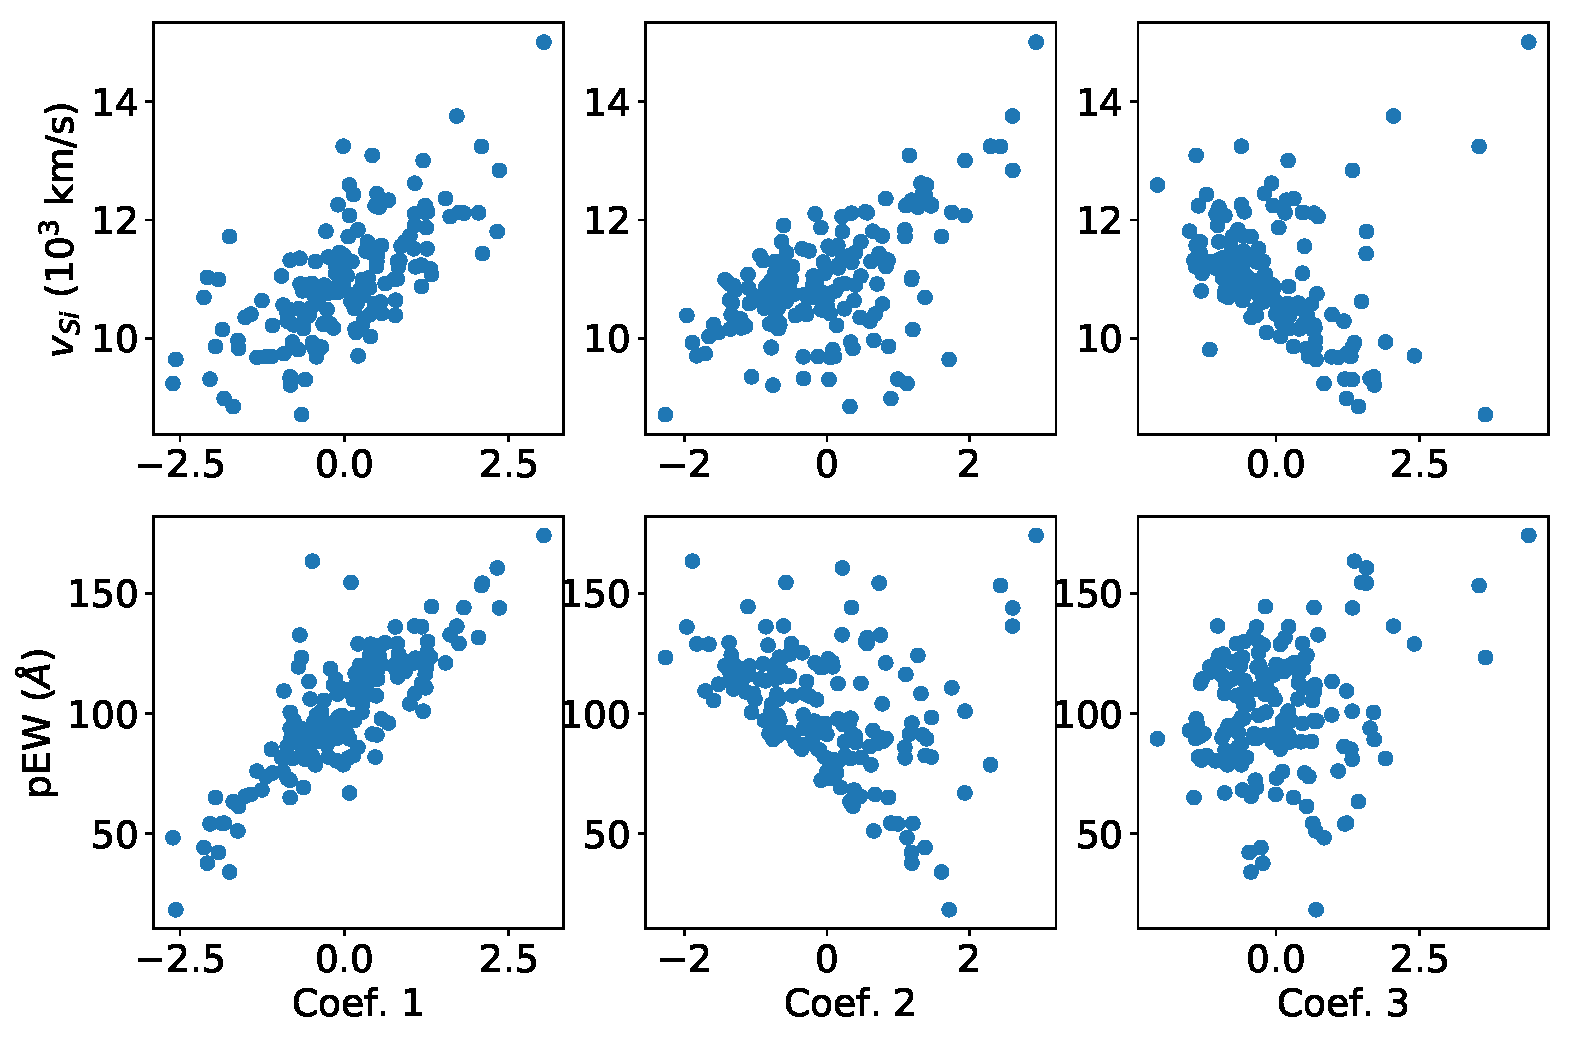
\includegraphics[width=0.9\textwidth]{figures/si_feat_pca/coef_vs_vel_and_ew.pdf}
    \caption{Scatter plots of the loading coefficients of the training data with their measured spectral indicators. We can see that each of the components is correlated with the velocity. Only the first two components are correlated with the pseudo-equivalent width.}
    \label{scatter_loading}
\end{figure}

\section{Validation}
\label{validation}

\subsection{Recovering Spectral Features at Native Resolution}
\label{snf_validation}
We can recover the spectral indicator measurements by reconstructing the full spectral feature from the EMFA model and measuring the velocity and equivalent width of the resulting reconstruction. When reasonably high resolution spectra are available, this reconstruction is unnecessary, so the native resolution recovery presented here is meant to provide a baseline estimate of how well the EMFA model can capture the inherently non-linear \siliconii{} features. It's real power will come into play when we estimate the velocity and pseudo-equivalent width from lower resolution or noisier spectroscopy.

Some examples of the feature recovery at native resolution are shown in Figure \ref{feature_recovery}. The histogram of residuals is shown in Figure \ref{snf_hist_resids_native_resolution}. The width of these distributions tells us how well the EMFA is capturing the spectral features. We find that the standard deviations (equivalently the root-mean-square or RMS) of these residual distributions are 369~km/s and 5.8~\AA{}, respectively. The normalized meidan absolute deviations\footnote{$$NMAD=1.4826\times\textrm{med}(|\bm{x}-\textrm{med}(\bm{x}|)$$} of these distributions are 253~km/s and 3.6~\AA{}. These errors in the recovery values are comparable to the average error on the original measurements (385~km/s for velocity and 6.8~\AA{} for the pseudo-equivalent widths).

\begin{figure}[htbp]
    \centering
    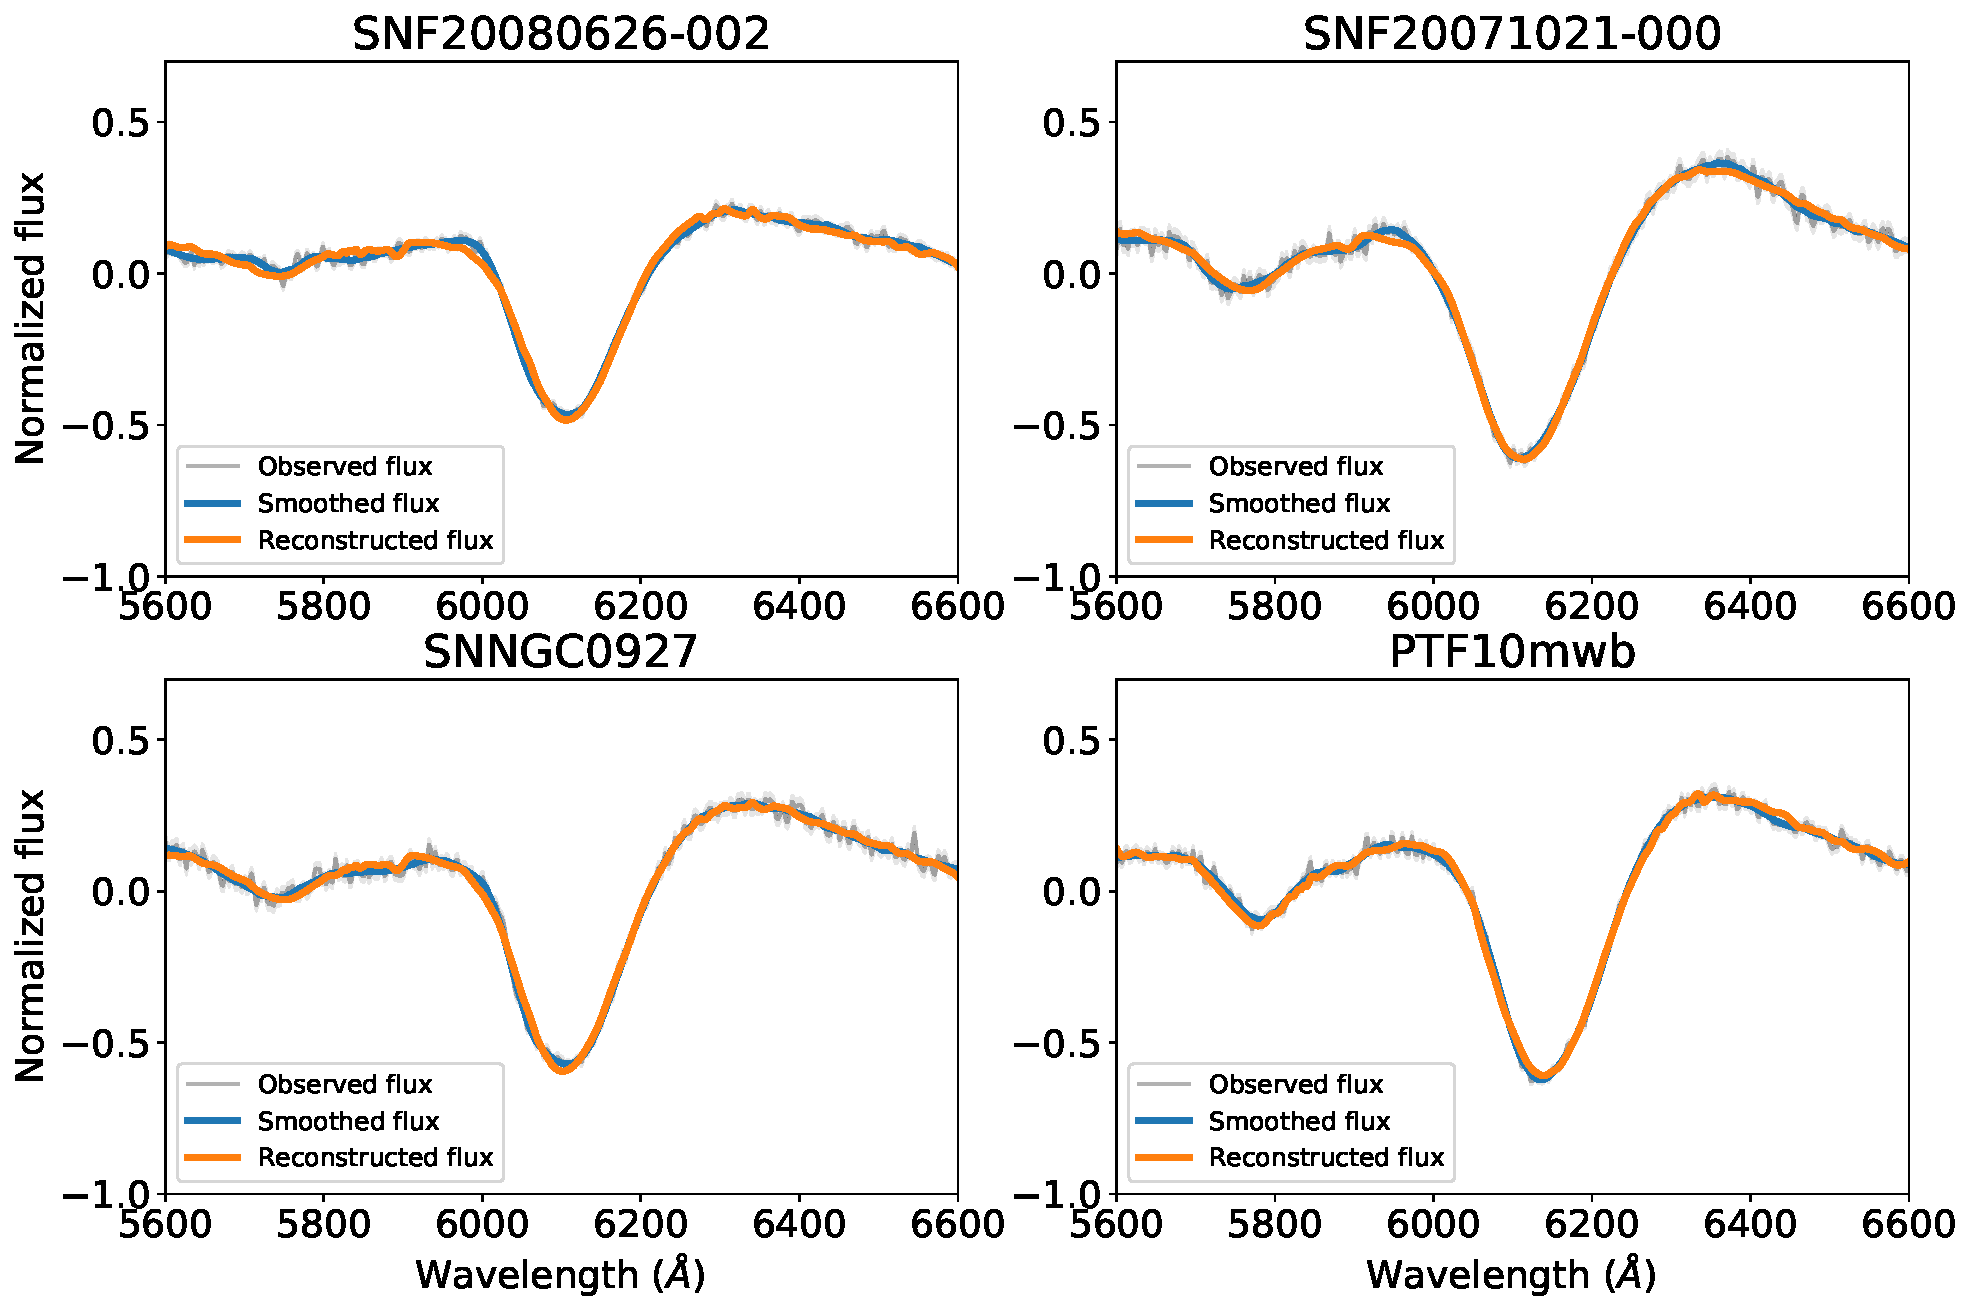
\includegraphics[width=0.9\textwidth]{figures/si_feat_pca/example_reconstruction.pdf}
    \caption{A random selection of recovered spectral features at the native resolution of the SNfactory spectra. The gray lines show the observed data, the blue line shows the data smoothed by the optimal Savitzky-Golay filter, and the orange line is the reconstructed flux.}
    \label{feature_recovery}
\end{figure}

\begin{figure}[htbp]
    \centering
    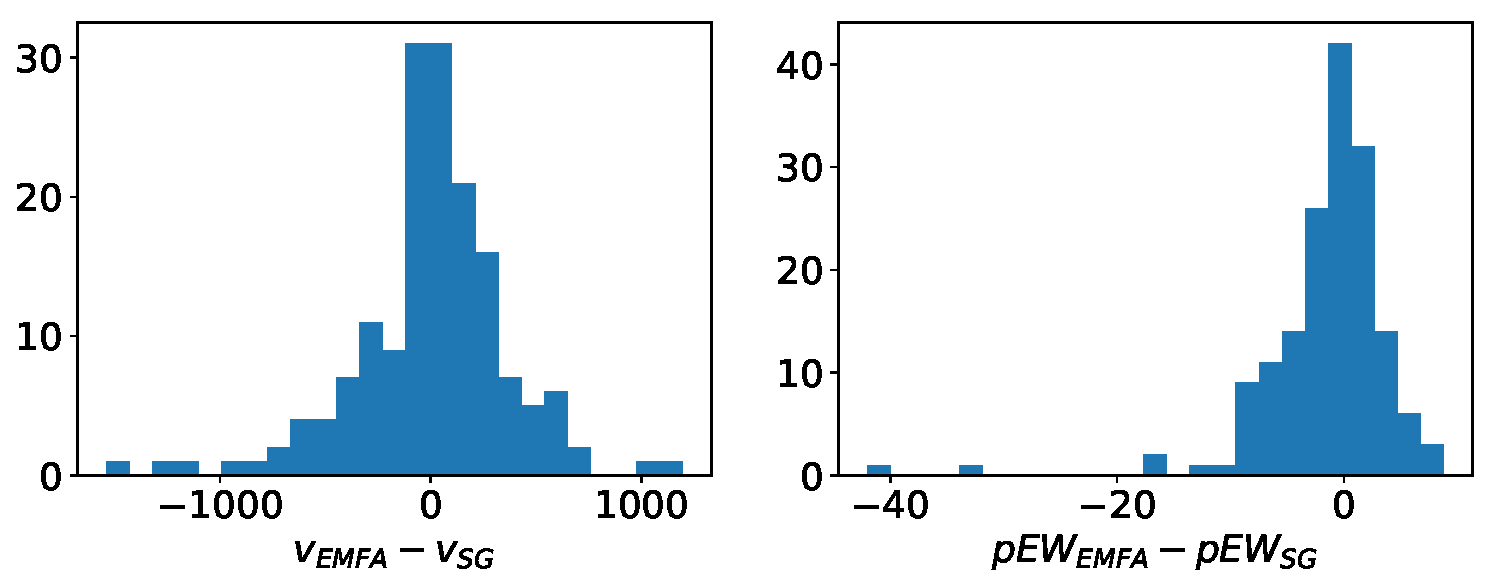
\includegraphics[width=0.9\textwidth]{figures/si_feat_pca/snf_recovery_resids.pdf}
    \caption{Histograms of the residuals between the velocities and equivalent widths measured from the flux reconstructed using the EMFA model and the original observed flux in the training data.}
    \label{snf_hist_resids_native_resolution}
\end{figure}

\section{Testing on External Data}
In order to ensure that our model is not overfit to our training data, we evaluate the effectiveness of our EMFA of the \siliconii{} feature on our external data set from the Berkeley SuperNova Ia Project \citep[BSNIP,][]{silverman_berkeley_2012} described in Section \ref{data}. Using the same techniques as in Section \ref{snf_validation}, we compare the velocities and pseudo-equivalent widths of the features inferred from the EMFA model and the true measured spectral indicators from the BSNIP spectra rebinned into a similar spectral resolution as the SNfactory training spectra. Figure \ref{bsnip_hist_resids} shows the residuals between the spectral indicators measured from the EMFA fits and the originally measured values. The spreads of these distributions are similar to the those of the training sample, with the standard deviations being 392~km/s and 7.7~\AA{} for the velocity and pseudo-equivalent widths, and NMADs of 355~km/s and 7.1~\AA{}. The results for both the SNfactory validation and the BSNIP test are all summarized in Table \ref{validation_results}.

\begin{figure}[htbp]
    \centering
    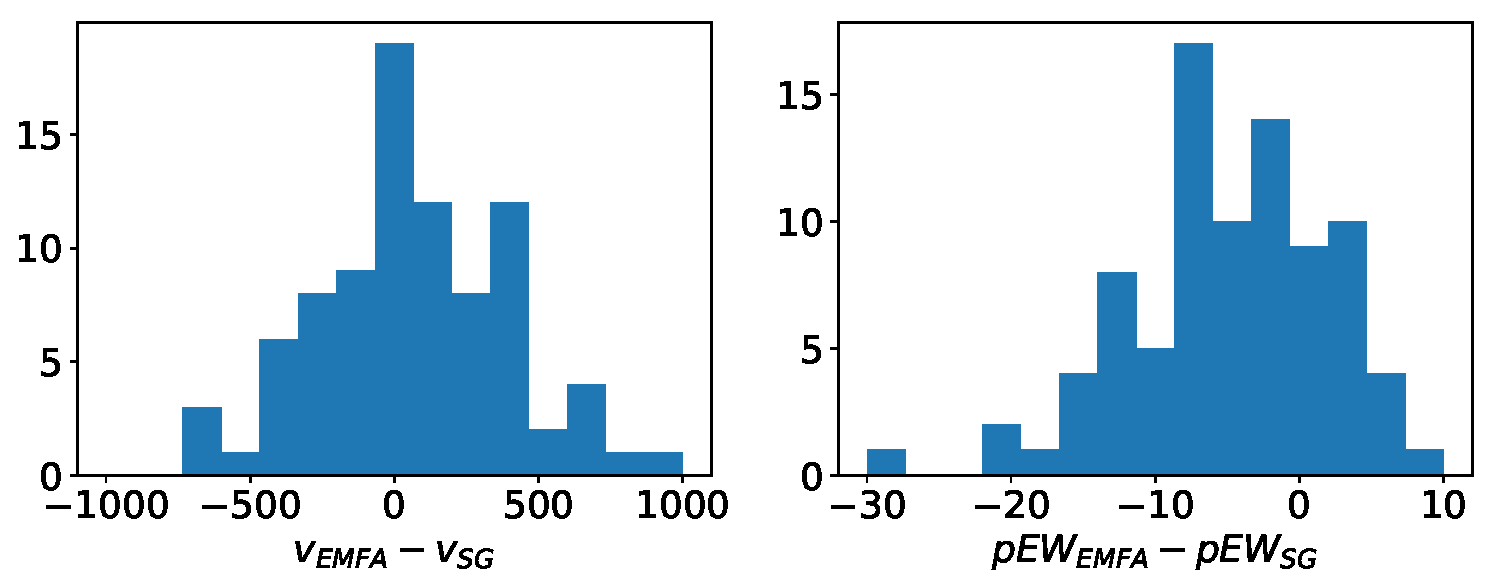
\includegraphics[width=0.9\textwidth]{figures/si_feat_pca/bsnip_recovery_resids.pdf}
    \caption{Histograms of the residuals between the velocities and equivalent widths measured from the flux reconstructed using the EMFA model and the original observed flux in the validation set. The outlier SN2005M has been removed from these plots (see Section \ref{outliers})}
    \label{bsnip_hist_resids}
\end{figure}

\begin{table}[htbp]
    \centering
    \begin{tabular}{ccccc}\\\toprule
        & \multicolumn{2}{c}{Velocity resids.} & \multicolumn{2}{c}{Equiv. width resids.}\\
        & \multicolumn{2}{c}{(km/s)} & \multicolumn{2}{c}{(\AA)}\\
        Data set & RMS & NMAD & RMS & NMAD\\\midrule
        SNfactory & 369 & 253 & 5.8 & 3.6 \\
        BSNIP & 392 & 355 & 7.7 & 7.1 \\\bottomrule
    \end{tabular}
    \caption{Measurements of the spread of the residuals between spectral features measured from the EMFA modeled spectra and spectral features measured from the true spectra for both the SNfactory (training) set and the BSNIP (test) set.}
    \label{validation_results}
\end{table}

\subsection{Investigating Outliers}
\label{outliers}
There are a few failed reconstructions from our validation. We show them in Figure \ref{valid_failures}, and discuss them here.

\begin{figure}[htbp]
    \centering
    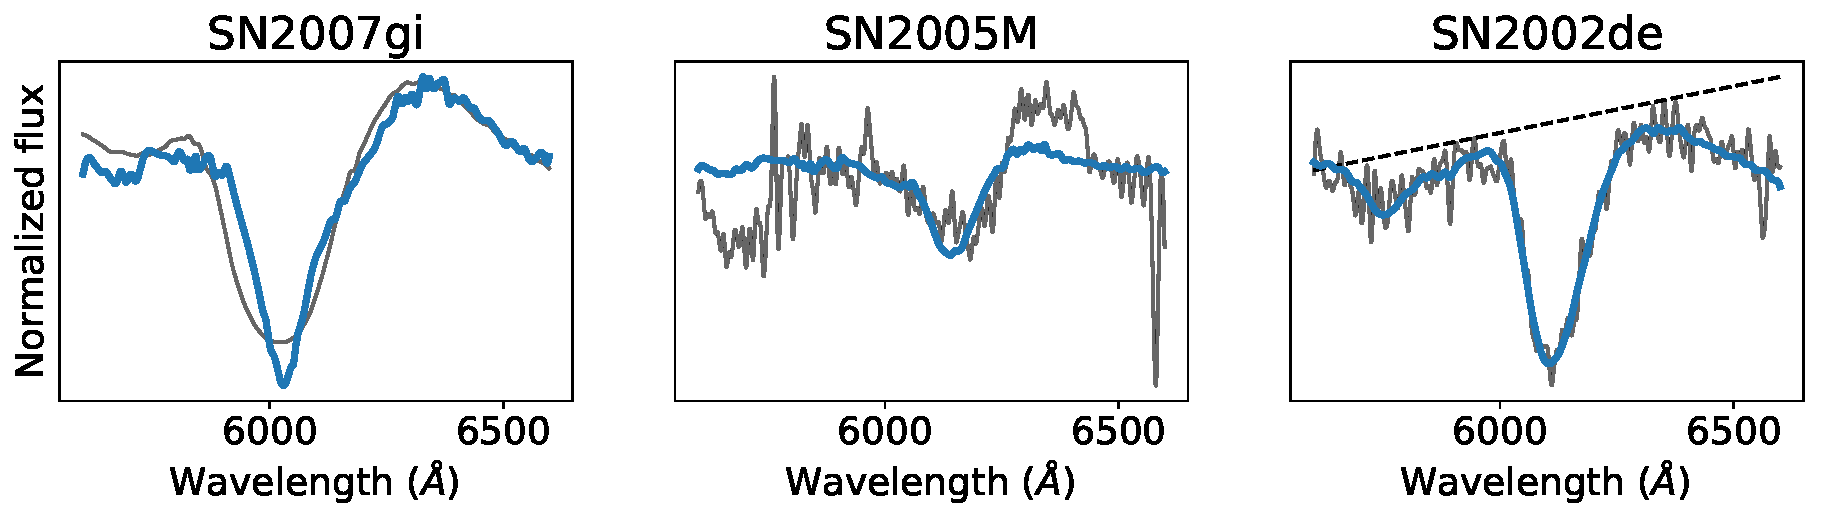
\includegraphics[width=\textwidth]{figures/si_feat_pca/fit_failures.pdf}
    \caption{Validation spectra where the EMFA fit and/or pseudo-continuum determination failed. The left frame is SN2007 gi, an exremely rapidly expanding object. The middle frame is SN2005M, which may be 1991T-like. The right frame shows an example of an object for which the pseudo-continuum determination failed due to underestimated variance in the spectrum. In each subfigure, the gray line represents the SG smoothed flux, and the blue line shows the best-fit EMFA flux. In the right figure, we also show the pseudo-continuum as a dashed black line.}
    \label{valid_failures}
\end{figure}

SN2007gi was a very well observed object with a high signal-to-noise spectrum, and thus precise measurements of the spectral indicators. Though the size of the residual was within the usual uncertainty of a measurement from a moderately well-observed spectra, the residual for this object was significantly larger than the measurement uncertainty. Looking at the recovered flux, we see that the EMFA model flux doesn't match the observed flux. SN2007gi is an extremely high velocity object ($v_{Si}=15740\pm180$~km/s with a large equivalent width ($pEW=176.9\pm1.6$~\AA{}), indicating that we may be somewhat limited by the diversity of our training set.

SN2005M was also a significant outlier. SN2005M has the shallow silicon lines of a SN1991T-like object, but a low velocity ($8300\pm 260$~km/s) that is uncharacteristic of SN1991T-like objects, which have typical velocities of $\sim 10000$~km/s \citep{blondin_spectroscopic_2012}. Since such shallow line objects were explicitly excluded from our training data set, the model is unable to capture this variation.

By eye checks of the remaining objects with large pseudo-equivalent width residuals reveal that it is not the EMFA that is failing to capture the feature, but failures in the pseudo-continuum determination in the SG filtering process. Usually, this is due to the variance spectra being underestimated, resulting in undersmoothing of the curve, and the limits of the pseudo-continuum being determined by noise spikes. An example of this is shown in the final panel of Figure \ref{valid_failures} for SN2002de.

\section{Simulated Roman Prism Spectra}
\label{wfirst}
\subsection{Generating Roman Prism Spectra}
The Nancy Grace Roman Space Telescope (hereafter Roman) is a future space telescope mission designed to constrain cosmological parameters with wide-field optical and near-infrared imaging. In addition to the imaging instrument (the Wide Field Channel, or WFC), a low-dispersion slitless prism has also been proposed as a tool to obtain spectroscopy for SNe Ia.

The full details of the prism simulation we use in this section can be found in Rubin et al. (in preperation), but we will present a summary here. The prism is still in design stages, so we assume a similar dispersion to the previously proposed Integral Field Channel (IFC), but with narrower wavelength coverage (0.7 to 1.8 $\mu$m). The survey simulation assumes an exposure time of one hour per pointing. This yields the at-max signal-to-noise ratios shown in Figure \ref{snr_wfirst_prism}, where we report the average signal-to-noise ratio per pixel from 5600-6600~\AA{} in the rest frame (the wavelength region of interest for this chapter). The average signal-to-noise ratio is calculated for a normal SN Ia in 38 evenly spaced redshift bins from 0.125 to 1.175. It is worth noting that the parameters of this survey (the wavelength coverage, dispersion, exposure times, etc) have not been optimized in any way; this survey serves as a benchmark for the spectral indicator measurement technique discussed here. Future work can use these analyses to find a more optimal survey strategy and instrument design.

\begin{figure}[htbp]
    \centering
    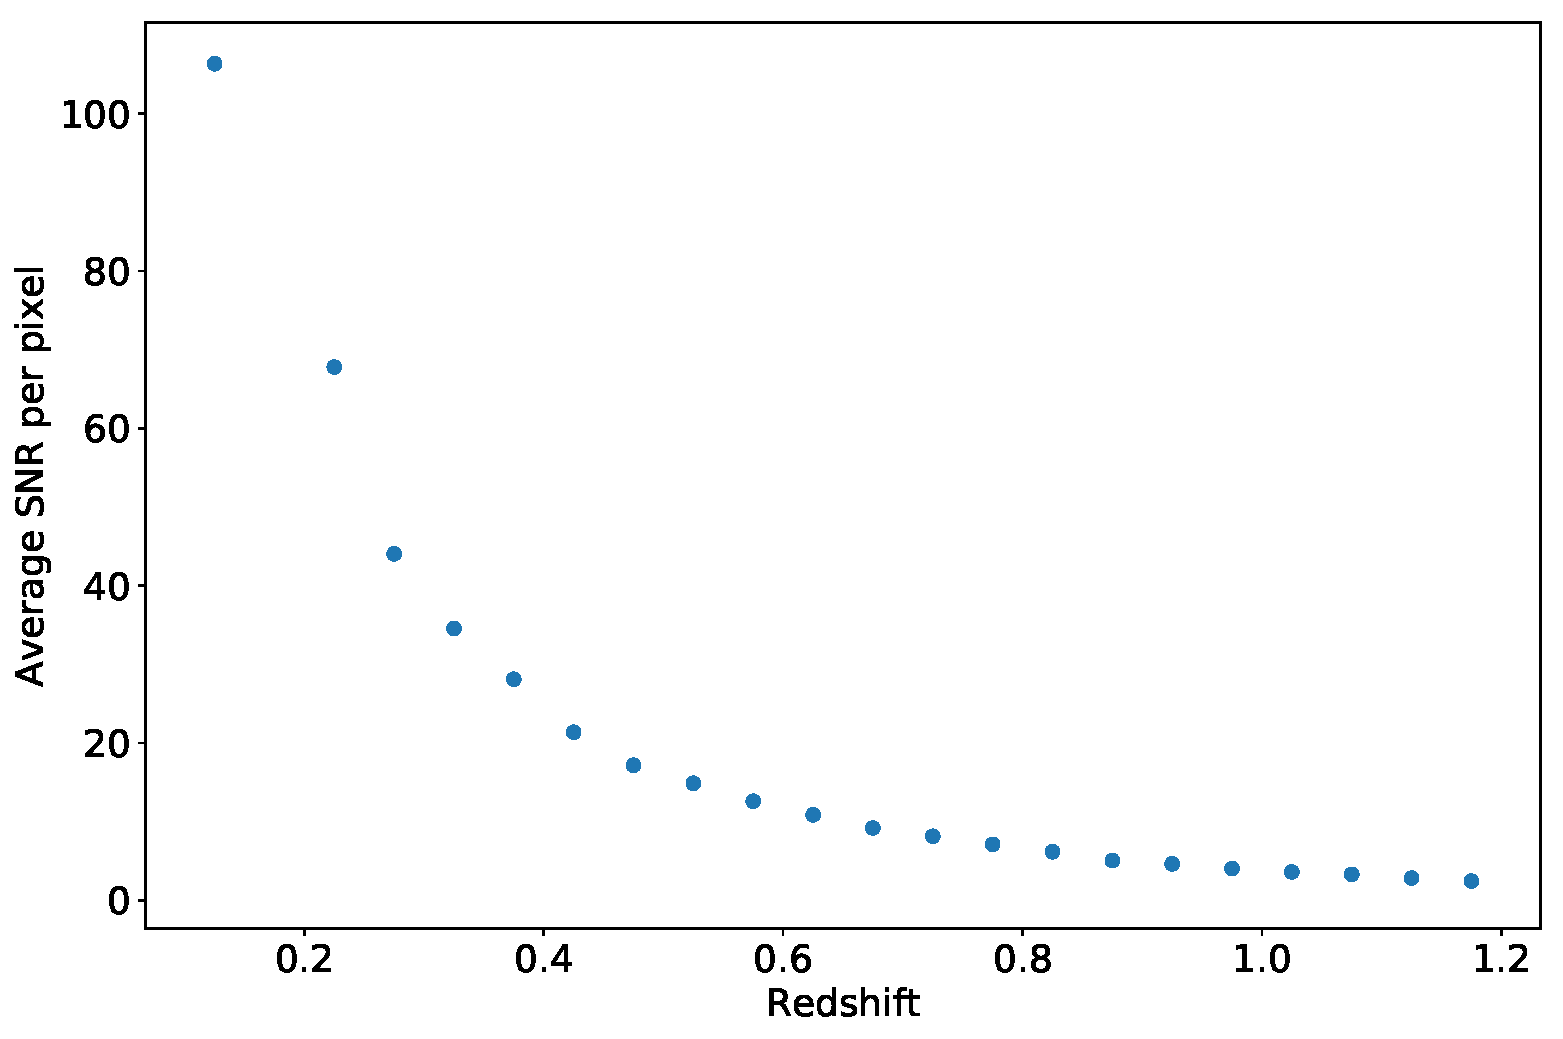
\includegraphics[width=0.9\textwidth]{figures/si_feat_pca/wfirst_snr_vs_redshift.pdf}
    \caption{Average signal-to-noise ratio for assumed for prism spectra used in the simulations. We report the average from 5600-6600~\AA{} in the rest frame since this the wavelength region of interest.}
    \label{snr_wfirst_prism}
\end{figure}

The simulated data set is generated as follows. For each object in the training set and for each redshift bin, we artificially redshift the spectrum to the redshift of the bin, resample the spectrum into the resolution of the prism spectrograph, and generate 50 realizations of the noise. The separate realizations allow us to inspect how the uncertainty (our confidence in the measurement value due to noise fluctuations) changes with redshift (or S/N) for spectra at these resolutions as well as how the errors (systematic offsets between the model and the true underlying data) change with redshift. A few example Roman prism spectra in a range of redshifts are shown in Figure \ref{wfirst_example_spectra}.

\begin{figure}[htbp]
    \centering
    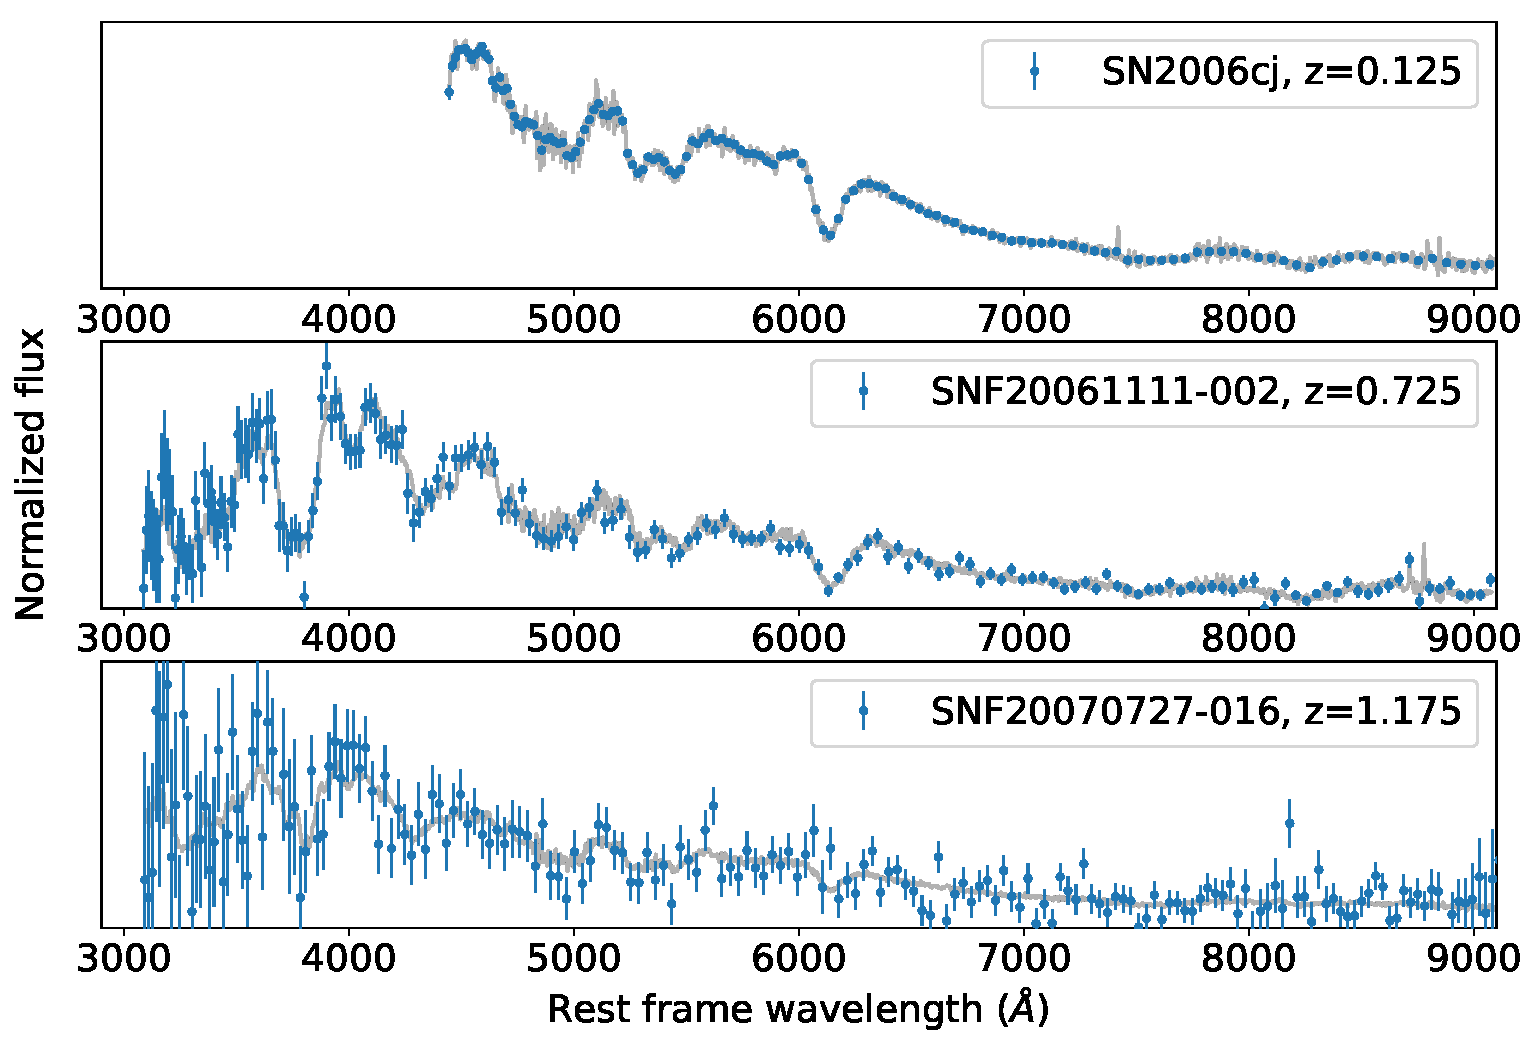
\includegraphics[width=0.9\textwidth]{figures/si_feat_pca/wfirst_example_spectra.pdf}
    \caption{Example realizations of the training set near-max spectra observed with the Roman prism spectrograph with a one hour exposure time.}
    \label{wfirst_example_spectra}
\end{figure}

Each of these spectra was preprocessed as described in Section \ref{data} and is available as part of the data repository accompanying this work.

\subsection{Spectral Indicator Recovery Results}
For every spectrum generated, we measured the velocity and pseudo-equivalent width using the SG smoothing, the Gaussian fit, and the EMFA fit methods. We then compared the results of these fitting methods to the true values of these spectral indicators (i.e. those measured from the original, high resolution, low noise spectra from the training sample).

In the validation step, the spectra we were fitting were at the same resolution as the training data. Therefore the data vectors had the same length and correspond to the same wavelengths as the training data, so we do not need to interpolate either the data or the model. Now we no longer have the same resolution, so we instead interpolate the model components using a spline and fit this interpolated model by minimizing
\begin{equation}
    \chi^2 = \displaystyle\sum_\lambda \frac{(f_{mod}(\lambda)-f_{obs}(\lambda))^2}{\sigma_{obs}^2(\lambda)}
\end{equation}
where $\lambda$ indexes the wavelength bins of the observation, $f_{mod}$ is the spline interpolated model spectrum evaluated at the wavelength bin $\lambda$, and $f_{obs}$ is the observed flux. An example of the recovered flux from one realization of one object is shown in Figure \ref{example_wfirst_recovery}.

\begin{figure}[htbp]
    \centering
    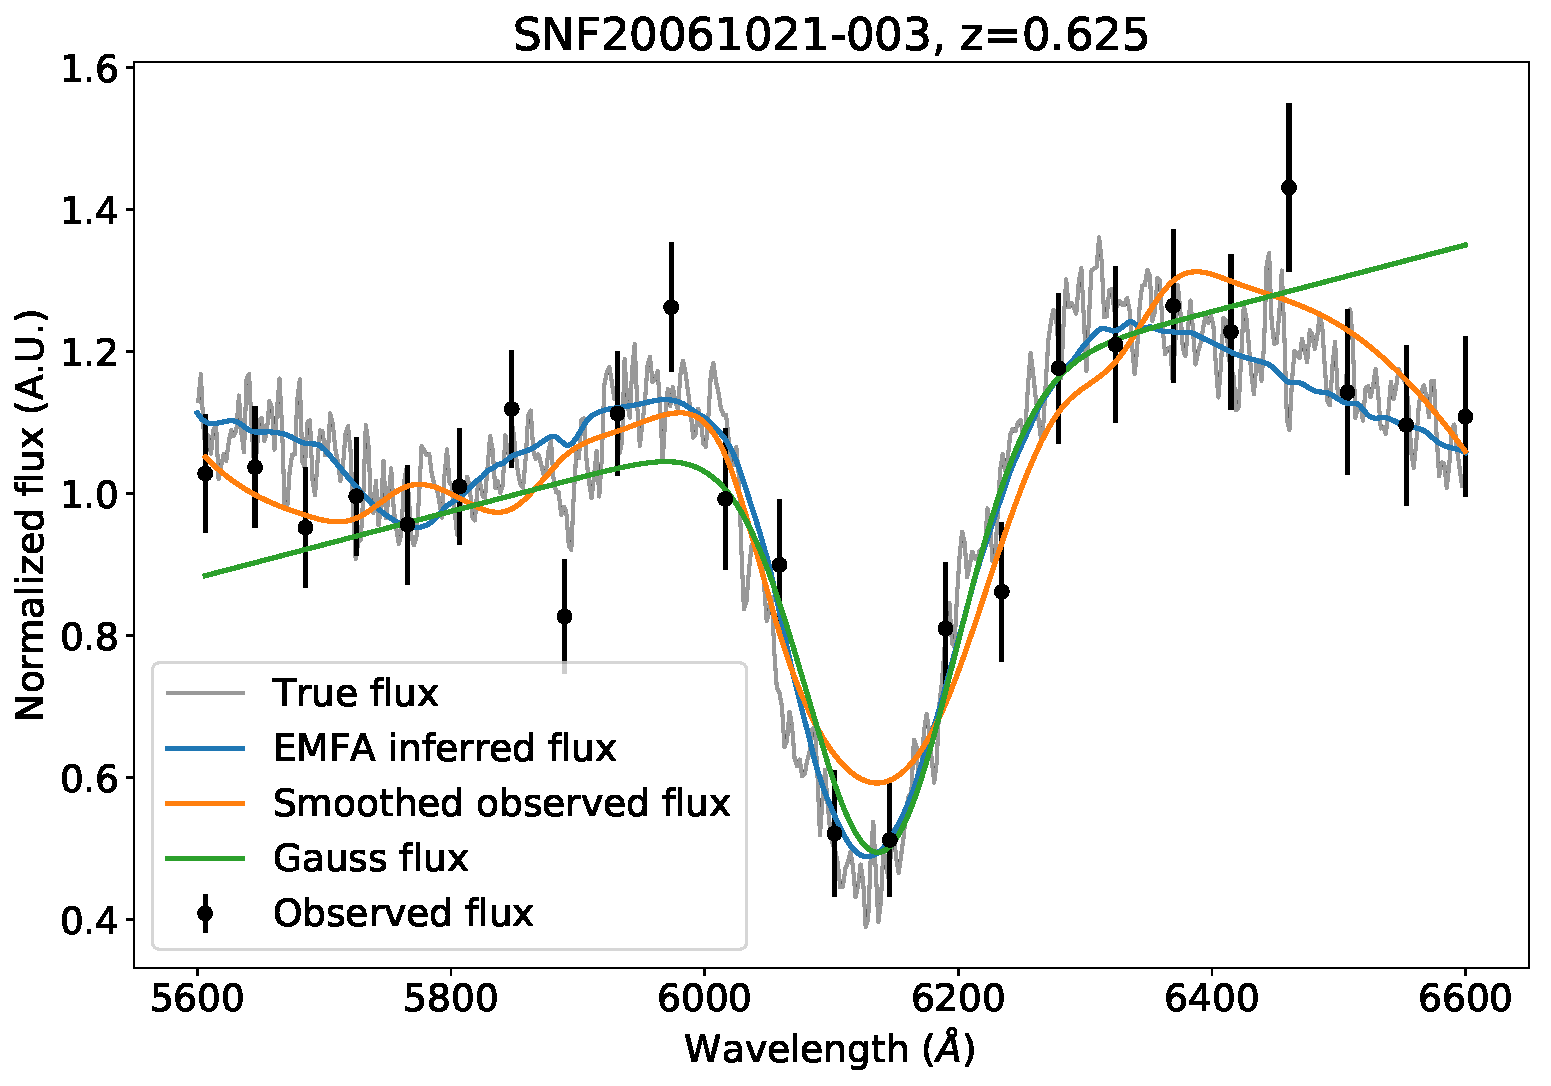
\includegraphics[width=0.9\textwidth]{figures/si_feat_pca/example_wfirst_emfa_recovery.pdf}
    \caption{Example of the various methods tested to recover the spectral indicators from the low resolution, noisy spectra from the Roman prism. The original training set spectrum that was resampled and noised is shown in gray. The realization of the prism observation (with uncertainties) is shown as the black data points. The best-fit EMFA spectral feature is shown in blue, the smoothed version of the observed flux is shown in orange, and the best-fit Gaussian line profile is shown in green.}
    \label{example_wfirst_recovery}
\end{figure}

First, we examine how the error in the measurements changes with redshift, where the error is defined by the difference between the measurements obtained from the noisy, degraded spectrum and the original data. Figure \ref{wfirst_vel_err_vs_z} and \ref{wfirst_ew_err_vs_z} show the average absolute difference between the velocities and pseudo-equivalent widths measured from the noisy data and those measured from the original data. At low redshifts (high signal-to-noise), each of the methods are roughly comparable. As the noise increases, though, the EMFA reconstruction does significantly better at recovering both the velocities and equivalent widths.

\begin{figure}[htbp]
    \centering
    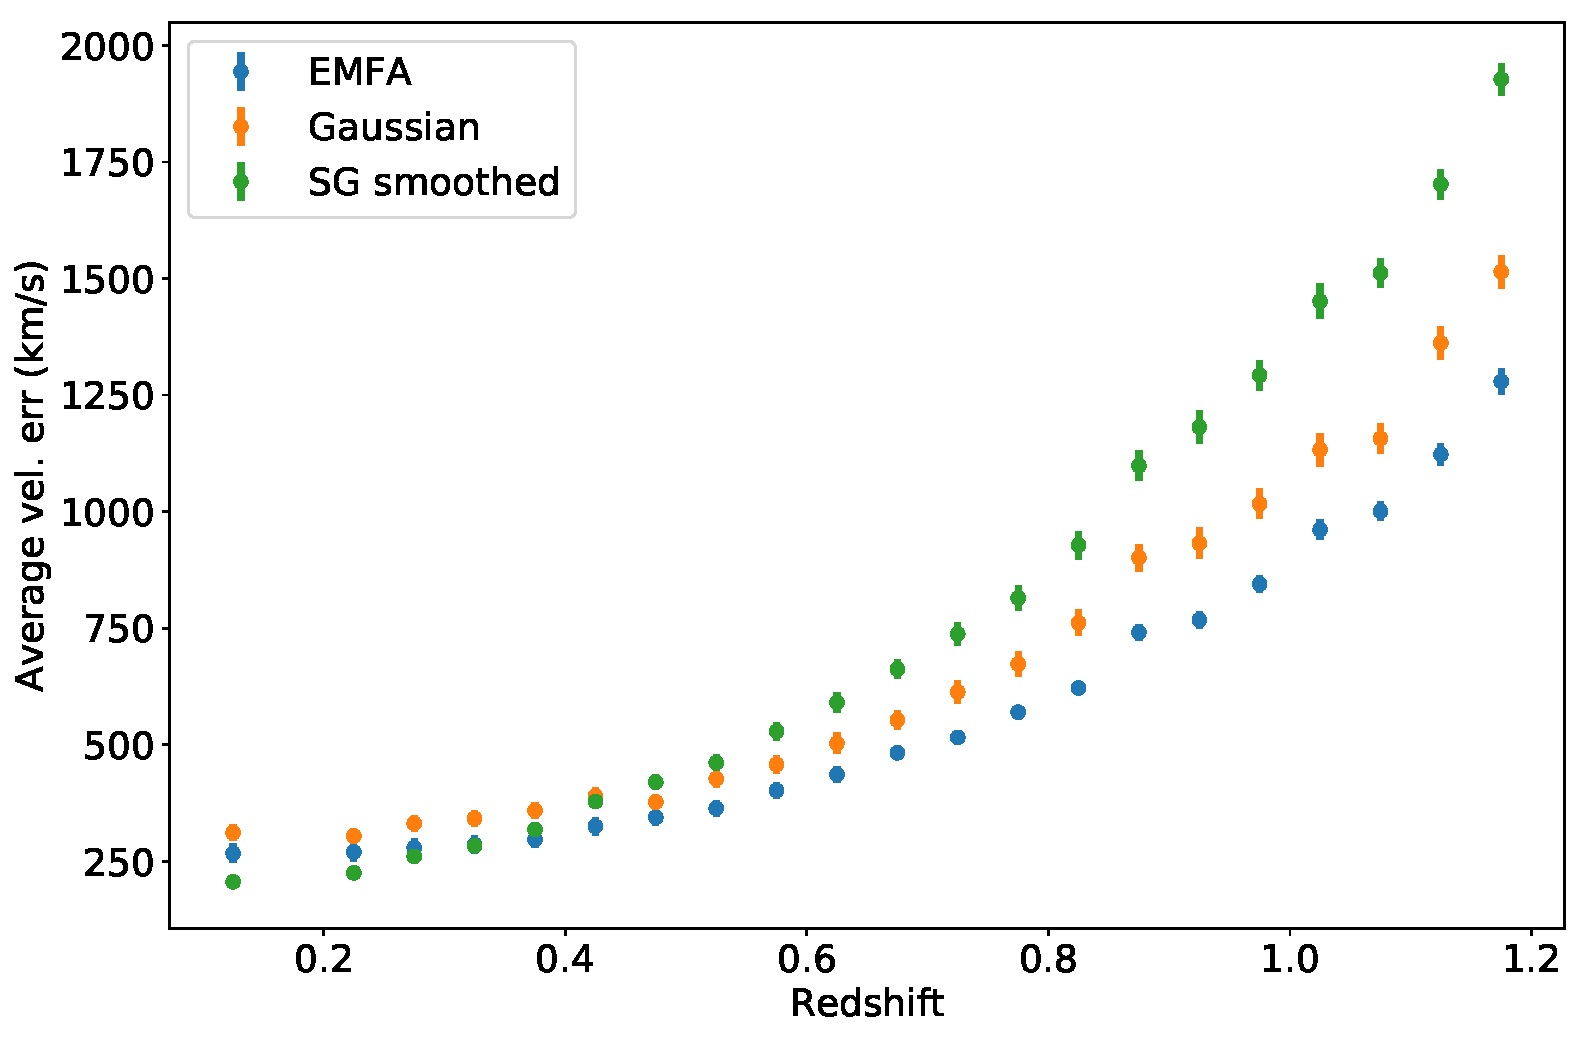
\includegraphics[width=0.9\textwidth]{figures/si_feat_pca/wfirst_vel_err.pdf}
    \caption{Per-redshift-bin average of the absolute value of differences between measured velocities and true velocities as a function of redshift. At low redshifts, the SG filtering method captures the true value best, but as noise increases, the EMFA method outperforms all other methods.}
    \label{wfirst_vel_err_vs_z}
\end{figure}

\begin{figure}[htbp]
    \centering
    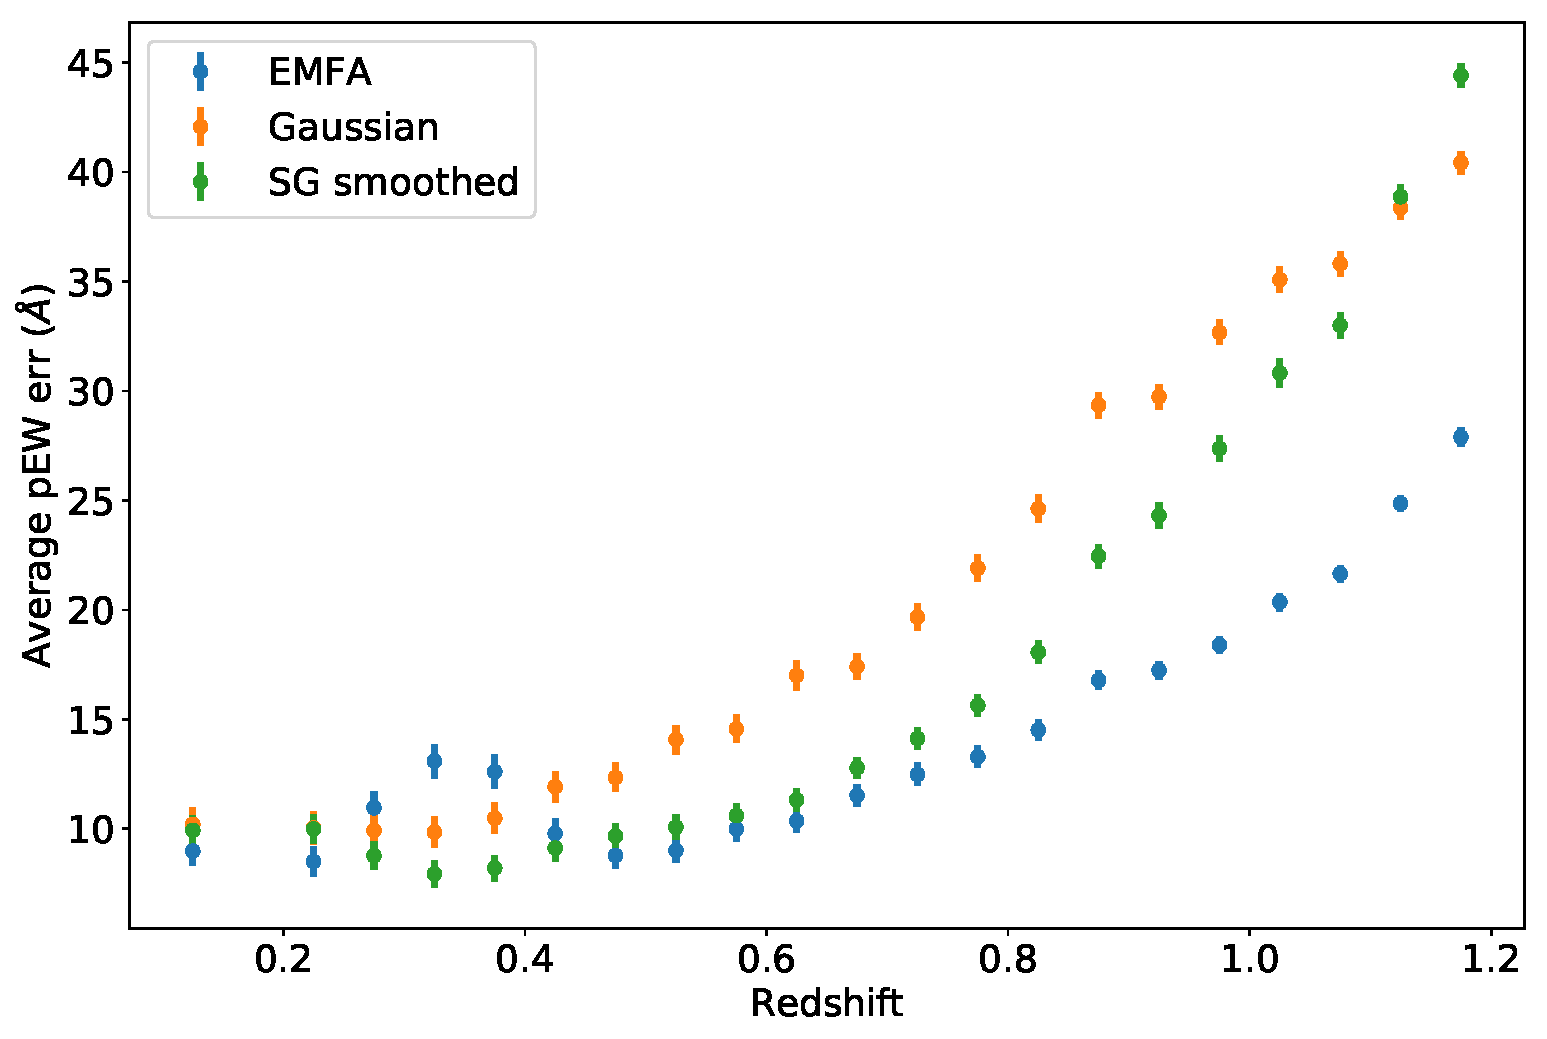
\includegraphics[width=0.9\textwidth]{figures/si_feat_pca/wfirst_pew_err.pdf}
    \caption{Same as Figure \ref{wfirst_vel_err_vs_z}, but for pseudo-equivalent width measurements. At low redshifts, all methods give comparable errors, but as the noise increases, the EMFA method is the preferred technique.}
    \label{wfirst_ew_err_vs_z}
\end{figure}

We also examine how the uncertainty in each of these measurements changes with the redshift in this prism survey. We look at the spread of the spectral indicator measurements among the 50 realizations of each object in each redshift bin. Figure \ref{wfirst_vel_uncertainty_vs_z} shows the average uncertainty of the velocity measurements as a function of redshift for each measurement technique. Figure \ref{wfirst_ew_uncertainty_vs_z} shows the same but for the pseudo-equivalent width measurements. Once again, we see that all measurement techniques are roughly comparable in both metrics at low redshift (high signal-to-noise). At higher redshifts, the EMFA outperforms the other techniques.

\begin{figure}[htbp]
    \centering
    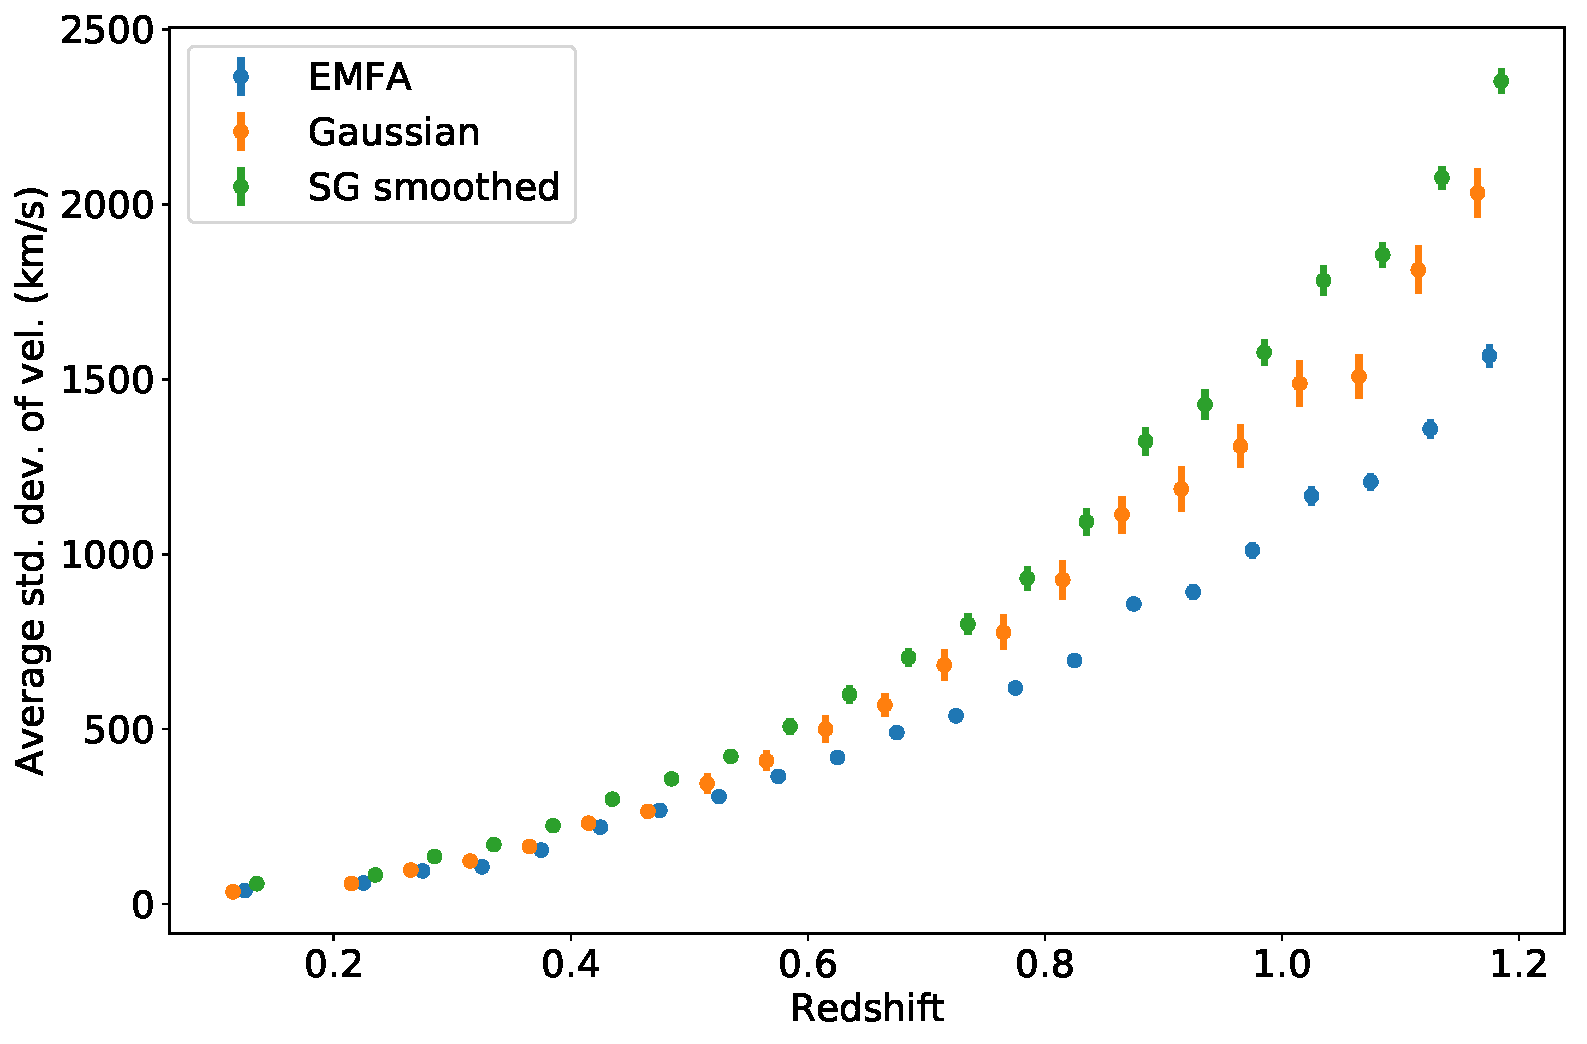
\includegraphics[width=0.9\textwidth]{figures/si_feat_pca/wfirst_vel_uncert.pdf}
    \caption{Per-redshift-bin average of the per-object standard deviations of the velocity measured with three techniques plotted as a function of redshift. The EMFA recovery technique outperforms both the Gaussian and SG filter smoothing techniques at all redshifts.}
    \label{wfirst_vel_uncertainty_vs_z}
\end{figure}

\begin{figure}[htbp]
    \centering
    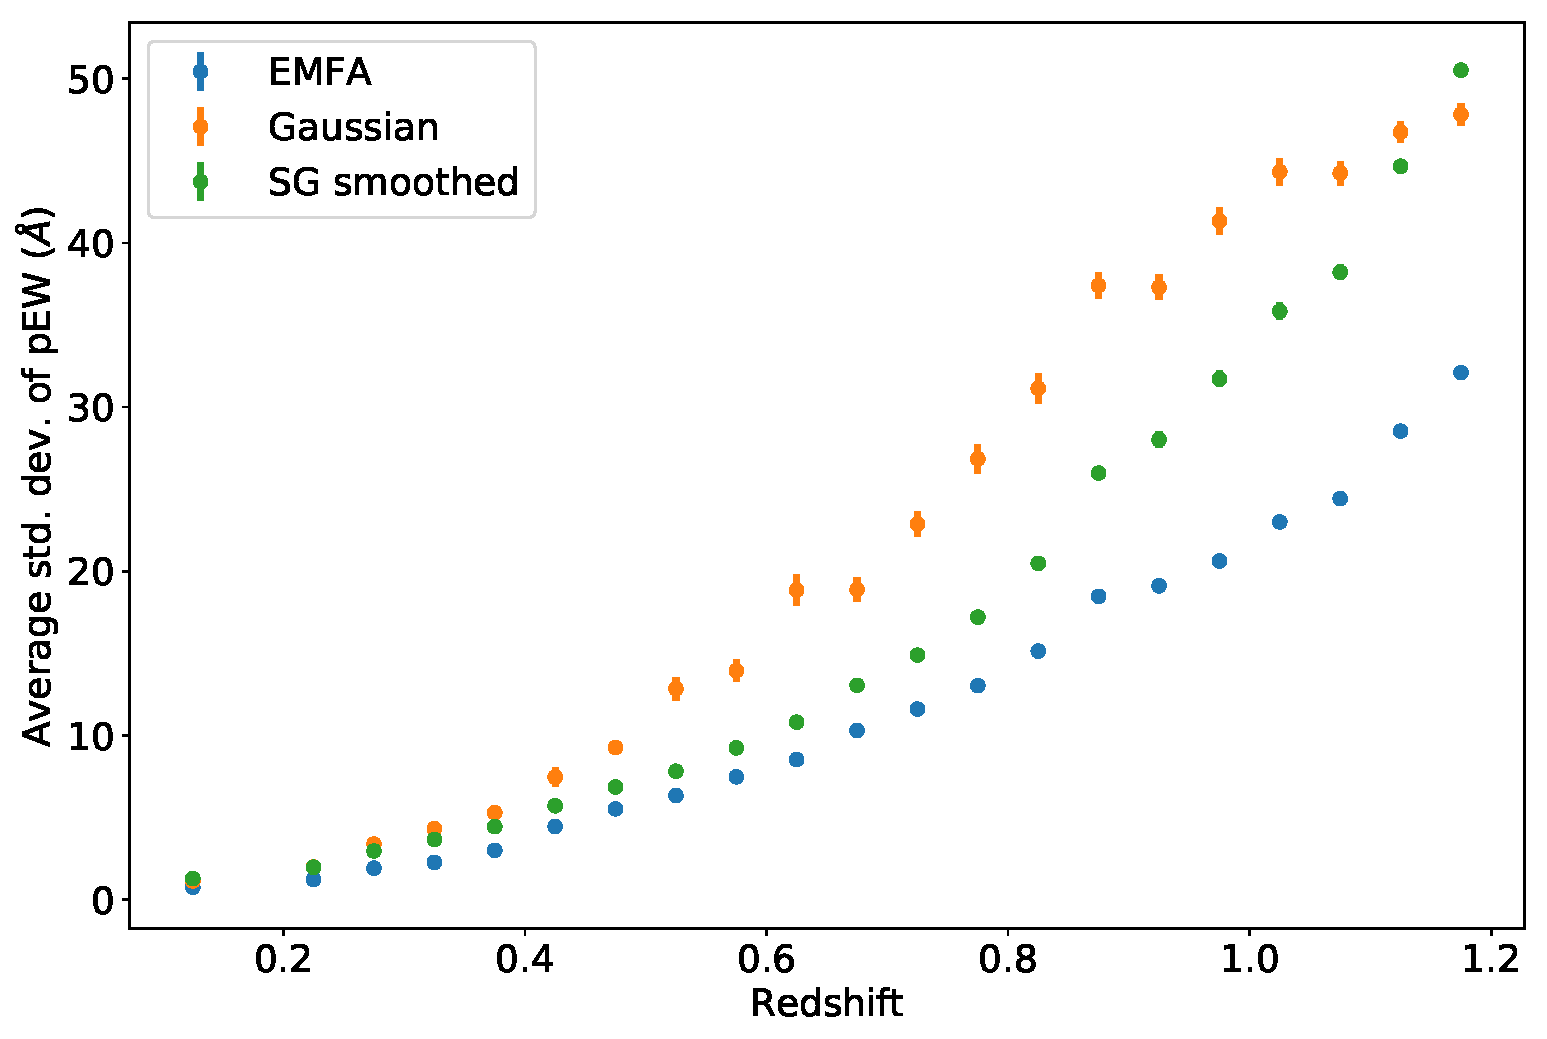
\includegraphics[width=0.9\textwidth]{figures/si_feat_pca/wfirst_pew_uncert.pdf}
    \caption{Same as Figure \ref{wfirst_vel_uncertainty_vs_z}, but for pseudo-equivalent width measurements. In contrast to the velocity measurement uncertainty, the SG filter smoothing methods seems to perform better than the Gaussian measurement in this metric. However, the EMFA still out-performs the both methods.}
    \label{wfirst_ew_uncertainty_vs_z}
\end{figure}

From this benchmark prism survey simulation, we find that our new method for recovering the \siliconii{} spectral indicators is both more precise and more accurate than other commonly used measurement techniques. By using a model of the feature informed by the data, we are able to extract more useful information from noisier data, allowing us to obtain the same spectral information in shorter exposure times. 

\section{Conclusions}
\label{conclusions}
We have presented a new method for reconstructing the \siliconii{} spectral feature of Type Ia supernovae. By using available high-resolution spectroscopic data, we are able to recover the velocity and equivalent width of the feature in low-resolution, noisy spectra with more precision and accuracy than the other methods shown. We have validated our model on an outside data set to ensure that the model was not overtrained and could generalize to other data sets. We also tested the performance of the model on simulated lower-resolution data for a range of signal-to-noise ratios as a benchmark, finding significant improvements in the measurement uncertainty and systematic error when using this new model instead of other techniques.

The results of the simulations can be used in future work to optimize cadence, observation, and instrument designs for upcoming supernova surveys. The improved performance in this metric could allow for more objects to be observed, or for even more accurate estimates of spectral indicators with the same exposure times. 

% There are several paths to extend this work. In our validation, we saw an example of the failure of the EMFA recovery technique to capture very broad, high-velocity features because of the lack of such examples in the training set. Future iterations of the with a larger and more diverse training set could remedy these types of failures. Another logical extension to this work would be to repeat this analysis for other spectral features (e.g. Ca II H\&K), or to go beyond observations near max and build a model of the temporal evolution of these features. Dixon et al. (in preparation) will continue this generalization, by using SNEMO \citep{saunders_snemo_2018} (an EMFA of full spectral time-series of SNe Ia) to recover a variety of spectral indicators from spectra observed at a range of phases or from photometric measurements.

\chapter{Kernel Density Estimates for Generating Mock Type Ia Supernova Observations with SALT2 and SNEMO}

\section{Introduction}
Type Ia supernovae (SNe Ia) remain one of the best cosmological distance indicators, allowing us to map out the expansion history of the Universe and understand the nature of the dark energy driving its accelerating expansion \citep{Perlmutter1999, Riess1998}. The power of SNe Ia stems from their status as ``standardizable candles`` -- their intrinsic luminosity is empirically correlated with other observable properties, like the light-curve width and color. Several large samples of SNe Ia across a range of redshifts are now available. These samples are large enough that the statistical errors are sub-dominant to systematic errors stemming from imperfect calibration and standardization.

Currently, the most common method for calibrating supernova brightnesses for cosmology uses the SALT2 model of \cite{Guy2007} along with an assumed linear relationship between the model parameters and absolute magnitude. The SALT2 model assumes that the flux $f$ in a given wavelength $\lambda$ at phase $p$ is given by
\begin{equation}
    f(\lambda, p) = x_0 \left[M_0(\lambda, p) + x_1\;M_1(\lambda, p)\right] \times \exp\left[c\;CL(\lambda)\right]
    \label{eqn:salt_flux_model}
\end{equation}
where $x_0$, $x_1$, and $c$ are parameters approximately describing the overall scale, light curve decay rate, and color of each supernova respectively, $M_0$ and $M_1$ are functions of phase and wavelength describing the average and typical variance of all supernovae, and $CL$ is a function of wavelength, representing the effects of both intrinsic and extrinsic color variation on observed flux. In a typical analysis, each observed light curve is fit with this model, giving $x_0$, $x_1$, and $c$ values for each supernova. The distance modulus to each supernova is then modeled by
\begin{equation}
    \mu = m_B^* + \alpha x_1 -\beta c - M
\end{equation}
where $m_B^*$ is the apparent magnitude in the Bessell B-band at maximum brightness of a supernova with the observed $x_0$, $x_1$, and $c$ (as predicted by the SALT2 model), and $\alpha$, $\beta$, and $M$ are nuisance parameters obtained from a simultaneous fit of $\mu$ and the distance modulus as a function of cosmological parameters. This linear relationship between supernova light curve parameters and magnitude is known as the Tripp relation \citep{Tripp1999}. After parametrizing the light curves with the SALT2 model and accounting for empirical relations between these parameters and luminosity with the Tripp relation, there still is scatter of approximately 0.14 mag remaining in the standardized magnitudes. Some portion of this scatter may be intrinsic, but several studies have shown that at least some of the scatter stems from flawed assumptions of the model.

Firstly, the light curve parametrizations themselves do not capture all of the diverse ways that observable supernova properties correlate with luminosity. The supernova twins analysis of \cite{Fakhouri2015} points to this particular problem with the standard SALT2 analysis pipeline by showing that directly comparing maximum brightness spectra, without any parametrization of the broadband light curves, results in a smaller scatter in standardized brightnesses. The existence of spectral subclasses of Type Ia supernovae (e.g. \cite{Branch2006}) and the relationship between ejecta velocities and Hubble residuals \citep{Siebert2020} also suggest that there is more information contained within the spectra of SNe Ia than the SALT2 model is capturing. The SuperNova Empirical Models (SNEMO, \cite{Saunders2018}; described in more detail in Section \ref{sec:data}) were introduced in part to mitigate the effects of using such incomplete models of supernova variation by including additional time-series flux components.

Even with a perfectly descriptive supernova flux model, the linear Tripp relation may be unable to capture all of the details of the relationship between light curve parameters and luminosity, resulting in additional unexplained dispersion in standardized magnitudes. For example, \cite{Rubin2015} found a preference for a broken-linear relationship between light curve color and luminosity. This issue has been significantly less well-studied than the inflexibility of the flux models, but further studies would require improved simulations to understand the relative fraction of uncertainty stemming from the inflexibility of the flux parametrization model as opposed to the standardization model.

Both of these issues are further complicated by selection effects and observational error. Without accounting for these uncertainties and propagating them through the analysis, the resulting cosmological parameter measurements are potentially biased. In order to have accurate simulations to quantify and correct for these biases, we must have a data-informed model of the underlying parameter populations. Indeed, \cite{Scolnic2016} show that using incorrect estimates of the underlying stretch and color distributions of the SALT2 parameters results in a small bias in the dark energy equation-of-state parameter, $w$. Simulations are an important tool in quantitatively disentangling the intrinsic scatter from the flux parametrization error and supernova standardization error; creating tools for more descriptive simulations is the main motivating factor of this work.

In this analysis, we present a tool for flexibly estimating the underlying population distributions of the model parameters for the SALT2 and SNEMO models in order to build accurate simulations that can address some of these issues. We present an overview of the SNEMO model in Section \ref{sec:snemo} and discuss the collection of spectro-photometric time-series data that we use throughout the analysis in Section \ref{sec:data}. In Section \ref{sec:kde}, we present the general framework for estimating latent joint probability distributions and the methods for quantitatively comparing these estimates to the simpler distribution estimation models like a multivariate Gaussian. We apply this methodology to our data and explain how to move from these parameter distribution estimates to mock observations in Section \ref{sec:making_mocks}. We compare the distributions of maximum-brightness spectral feature measurements in Section \ref{sec:spec_diversity}, and conclude with some proposed further analyses in Section \ref{sec:conclusions}.

\section{SNEMO}
\label{sec:snemo}
The SuperNova Empirical MOdels (SNEMO) are a family of linear models that were built to capture more of the spectral variation than is captured by lower-dimensional models like SALT2. The flux at wavelength $\lambda$ and phase $p$ is modeled by
\begin{equation}
    f_\text{mod}(\lambda, p) = c_0 \left[e_0(\lambda, p) + \displaystyle\sum_{i=1}^k c_i\;e_i(\lambda, p)\right] \times 10^{-0.4 A_s CL(\lambda)}
\label{eqn:snemo_flux_model}
\end{equation}
where $e_0(\lambda, p)$ is the average spectral sequence, and each of the $e_i(\lambda, p)$ represent orthogonal aspects of spectral variation. $CL(\lambda)$ is the \cite{Fitzpatrick1999} dust law and is fixed across all time scales to represent extinction from dust. The model parameters are then the overall scaling $c_0$, the variational parameters $c_i$ and the dust-reddening parameter $A_s$. These $k+1$ parameters represent the full spectral time-series data in the model space, similar to how the parameters $\{x_0, x_1, c\}$ represent a time-series of spectra in the SALT2 model.

\cite{Saunders2018} presents three different variations of the model, each with different numbers of parameters and intended for different uses. SNEMO2 has a single spectral variation vector ($k=1$) in addition to the overall scale and color parameters, and serves as a point of comparison to the commonly used SALT2 model. SNEMO7 has six spectral variation vectors ($k=6$) and is presented as a model for supernova standardization, as it minimizes the unexplained dispersion in standardized magnitudes of supernovae after using the coefficients of this model to linearly standardize the luminosity. Finally, SNEMO15 ($k=14$) is presented as a model to explain as much of the spectral variability as possible, as measured by the total $\chi^2$ difference between the model and the observed fluxes at all of the modeled wavelengths and phases. Throughout this work, we make use of and compare these three models along with the SALT2 model.

\section{Data}
\label{sec:data}
In order to generate new spectral time-series data, we first need measurements of the model parameters from a representative data set. The representative data set we are using throughout this analysis is the spectral time-series data from the Nearby Supernova Factory (SNfactory). SNfactory has collected spectrophotometric time series data from over 400 SNe Ia. Of these, 228 are considered high quality enough for light curve fitting. For each model (SALT2 and each SNEMO model), we obtain a vector of model parameters for every supernova by minimizing
\begin{equation}
    \chi^2 = \displaystyle\sum_{\lambda, p} f_\text{obs}(\lambda, p) - f_\text{mod}(\lambda, p\;|\; \Theta)
\end{equation}
with respect to the model parameters $\Theta$, where $f_{obs}$ is the observed flux (after correcting for Milky Way dust extinction), and $f_{mod}$ is the model flux from Eqn. \ref{eqn:snemo_flux_model} in the case of the SNEMO models or Eqn. \ref{eqn:salt_flux_model} for SALT2.

The overall scaling parameter ($c_0$ for the SNEMO models and $x_0$ in the SALT2 model) measured for each supernova depends not only on the absolute magnitude of the object, but also on the object's redshift. We would like our generative model to be able capture the range of intrinsic absolute magnitude fluctuations irrespective of the redshift and to include correlations between these fluctuations and the spectral model parameters. To accomplish this, we convert these scaling parameter value to a value representing the absolute magnitude of each object, $M_B^*$, by calculating the apparent magnitude in the Bessell B-band at maximum brightness of a supernova with the best-fit $c_i$ and $A_s$ values and subtracting the distance modulus to an object at the same redshift assuming a fixed, fiducial $\Lambda$CDM cosmology with $H_0=70$ km/s/Mpc and $\Omega_{m}=0.3$. To simplify our plots and our kernel density estimates, we subtract a typical value of this parameter ($\langle M_B^*\rangle = -19.1$).

Table \ref{tab:snemo_coefs} presents a truncated table wit the SALT2, SNEMO2, SNEMO7, and SNEMO15 coefficients for each supernova in the data set, along with their $M_B^*$ values. The full-table is available online.

\todo[inline]{make this table}

\begin{table}[h!]
    \centering
    \begin{tabular}{c|c}
        xx & xx \\
        xx & xx
    \end{tabular}
    \caption{}
    \label{tab:snemo_coefs}
\end{table}

\section{Kernel Density Estimation}
\label{sec:kde}
With these measurements in hand, we move on to estimating the underlying joint probability distribution of these observations. Kernel density estimation is one such method for making these approximations. Simply put, it accomplishes this by weighting each of the observed data points by some kernel function $k(x_{1}, x_{2})$ and summing these weights to produce a smooth curve. Although the resulting estimate of the latent probability distribution is non-parametric, the kernel function used is usually parametrized by a parameter known as the bandwidth. This hyperparameter controls the level of smoothing by controlling the relative weights of data points spread further apart.

In this section, we lay out a pedagogical exploration of the details of this process, including bandwidth and kernel selection and complications stemming from higher data dimensionality, so that we can effectively apply this technique to the data.

\subsection{KDE in 1 Dimension}
\label{sec:1d}
Let's first consider the one-dimensional case. Fig. \ref{fig:1d_hist} shows a histogram for a series of observations drawn from an exponentially-modified Gaussian distribution. We choose this distribution to illustrate the impact of non-Gaussianity (in particular skewness) on the resulting estimates of the underlying probability distribution. The true probability distribution function is shown as a black line in Fig. \ref{fig:1d_hist}. The remaining lines in Fig. \ref{fig:1d_hist} show the resulting kernel density estimates using a Gaussian kernel with a range of bandwidth values. We can qualitatively see that a bandwidth of 0.53 results in an estimate that closely resembles the true probability distribution, while a value of 0.1 is too narrow (overfitting/high variance) and 3 is too wide (underfitting/high bias).

\begin{figure}
    \centering
    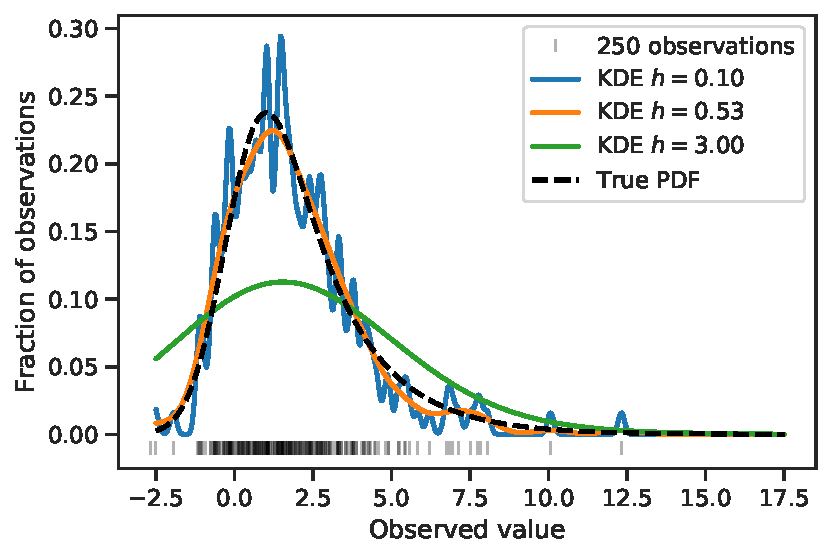
\includegraphics{figures/snemo_kde/1d_hist_example.pdf}
    \caption{Example of a kernel density estimate of a 1-dimensional, non-Gaussian distribution. The ticks represent the $n=250$ observations drawn from the true distribution shown with the black dashed line. The blue, orange, and green lines represent KDEs with increasing bandwidth sizes.}
    \label{fig:1d_hist}
\end{figure}

\subsubsection{Bandwidth Selection with Cross-validation}
There are some general rules-of-thumb for selecting an optimal bandwidth; for example, Silverman's rule of thumb:
$$h= 0.9\times\min\left(\hat{\sigma}, \frac{\textrm{IQR}}{1.34}\right) \times n^{-1/5}$$
where $\hat{\sigma}$ is the standard deviation of the sample, $\textrm{IQR}$ is the interquartile range of the sample, and $n$ is the number of data points in the sample \citep{Silverman1986}. This rule can perform quite well in most circumstances. However, these types of rules-of-thumb generalize quite poorly when the data is highly non-Gaussian (e.g. multi-modal distributions) or when the dimensionality of the data is high.

Another way to find the best bandwidth parameter is to try several values of the parameter and compare the results via some metric. A commonly used method for performing this type of evaluation is $k$-fold cross-validation. In $k$-fold cross-validation, we split the sample into $k$ groups. We then hold one of these groups out and train the model on the examples in the remaining $k-1$ groups. The model is then evaluated on the examples in the held-out set. This process is repeated until each example in the data set has been used in the training and validation. The overall model evaluation is then usually taken to be the mean of the evaluation metrics found in each of the cross-validation rounds, and the standard deviation of these metrics can be used to estimate the uncertainty on that metric.

A simple metric to use in the case of KDE is the sum of the log probabilities of the test data under the model. If the probability distribution resulting from the KDE is overfit (the bandwidth is too narrow), then the log probability of data points in the held-out set (which are drawn from the same underlying probability distribution) will be much lower than expected. The same would be true if the bandwidth was too wide and the model was underfitting the data, as long as the probabilities are normalized.

Using these techniques on our toy example from above, we find an optimal bandwidth of 0.53, as evidenced by the maximum at this point in Fig. \ref{fig:1d_bandwidth_opt}, plotting the total log probability of the $k$-folds as a function of bandwidth parameter.

\begin{figure}
    \centering
    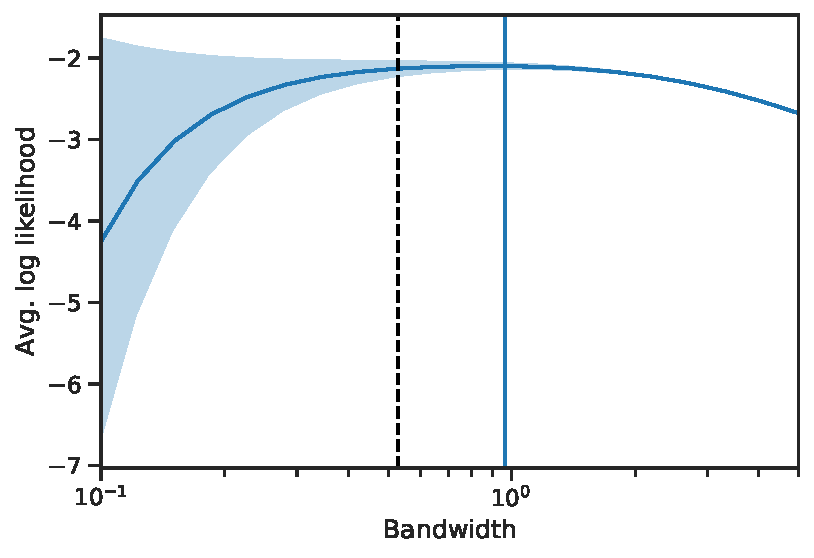
\includegraphics{figures/snemo_kde/1d_bandwidth_example.pdf}
    \caption{Results from 5-fold cross-validation for the example distribution and data shown in Fig. \ref{fig:1d_hist}. The blue line and shading show the mean and standard deviation of the normalized scores from all of the cross-validation subsets. The vertical blue line shows the location of the maximum score. The dashed black line shows the location of the Silverman's rule-of-thumb estimate for the optimal bandwidth.}
    \label{fig:1d_bandwidth_opt}
\end{figure}

\subsection[KDE in d Dimensions]{KDE in $d$ Dimensions}
The case in $d>1$ is quite similar to the 1-dimensional case. The kernel, though, is now in $d$ dimensions, and as such, the bandwidth is no longer a single parameter but a $d\times d$ symmetric matrix describing the bandwidth in each dimension along with the correlations between dimensions. The higher-dimensional case is further complicated by the so-called ``curse of dimensionality", where the sparseness of the data in the higher dimensional space causes the density estimate to converge more slowly. We will explore this first detail with a similar toy model to that used in \ref{sec:1d} but in 2 dimensions for ease of visualization.

\subsubsection{Transforming the Data for Bandwidth Estimation}
Consider a 2-dimensional sample drawn from a bivariate Gaussian distribution with mean $\bm{\mu}$ and covariance $\bm{\Sigma}$ (i.e. $(y_1, y_2)\sim\mathcal{N}(\bm{\mu}, \bm{\Sigma})$) and then consider a non-linear transformation to that sample, transforming $y_2$ to $z_2 = \exp(y_2)$. 

This example joint distribution is correlated and nonlinear, and as such works as a good test of the power and limitations of our methodology. We start by making estimates width a Gaussian kernel for a range of bandwidths as we did in the 1-dimensional case, giving us the results shown in Fig. \ref{fig:2d_scatter_unscaled}. However, the standard \verb|sklearn| implementation of the kernel density estimator incorrectly assumes that covariance matrix of the kernel is proportional to the identity matrix, so in our $k$-fold cross-validation, we are tuning a single bandwidth parameter $h$.

\begin{figure}
    \centering
    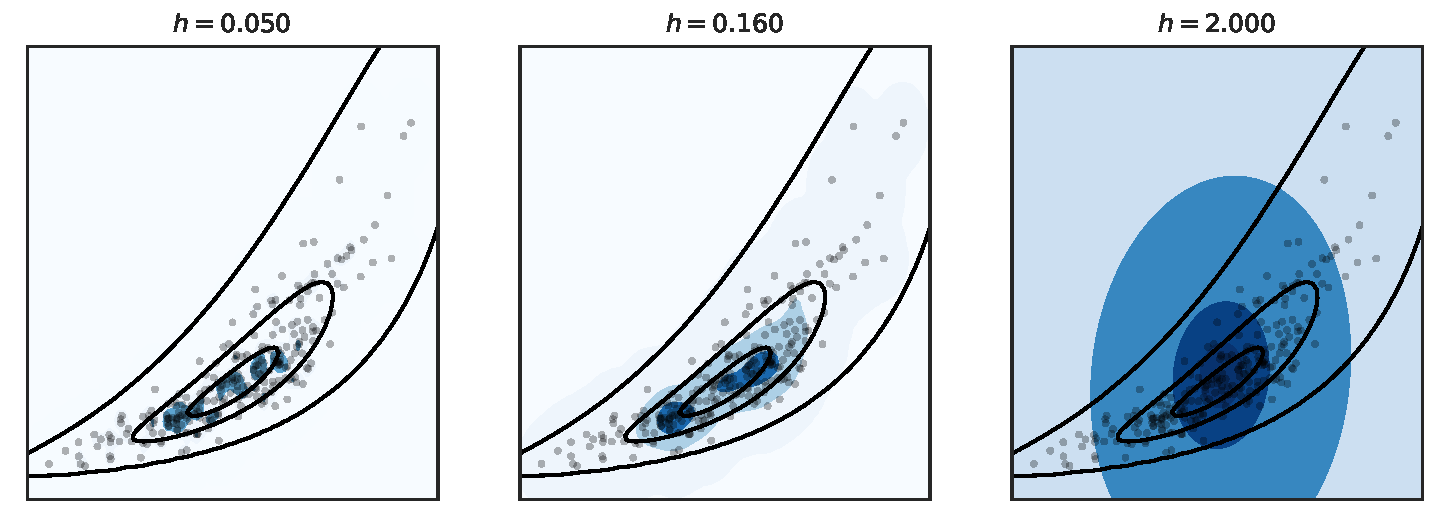
\includegraphics[width=0.9\textwidth]{figures/snemo_kde/2d_scatter_no_scaling.pdf}
    \caption{Example kernel density estimates in 2 dimensions for a joint probability distribution that is correlated and non-Gaussian. The $n=250$ data points are shown as black dots. The black contour lines show the true 1, 2, and 3 $\sigma$ contours, while the fading shades of blue show the 1, 2, and 3 $\sigma$ estimates of the KDE. In each of these examples, we assume a Gaussian kernel with no covariance terms.}
    \label{fig:2d_scatter_unscaled}
\end{figure}

We can see in the central panel of this figure that even the best-fit value of $h=0.143$ obtained from $k$-fold cross-validation is not a very good estimate of the true joint probability density. In particular, the density estimate makes the distribution appear multimodal. This occurs because the kernel does not reflect the full range of scales in the different dimensions of the space, so it takes on an $h$ value that reflects an average length scale.

We can improve our estimate by allowing the data to dictate the form of the kernel. We want to understand the relative fractions of the dispersion of the data in each dimension, as well as how the data covaries in each dimension. This will allow us to create a Gaussian kernel that is more reflective of the data, and therefore give us a better fit. We do this by finding a whitening transformation of the data, i.e. a transformation $W$ that turns our data matrix $X$ with covariance $\Sigma_X$ into a data matrix $Y=WX$ with covariance $\Sigma_Y=\mathbb{I}$. With this whitening transformation, we can reproject our data into whitened space, fit the KDE as usual, and then apply the inverse transformation to the KDE sample to obtain a KDE with a tuned kernel that matches the data.

A commonly used whitening matrix is $W = \Lambda^{-1/2}U^\top$, where $\Lambda$ is the diagonal matrix of eigenvalues and $U$ is the matrix whose columns are the eigenvectors of the covariance matrix $\Sigma_x$ (see proof in Appendix \ref{app:whitening_matrix_proof}). Using this transformation, we can complete the process of transforming our data, fitting the KDE, and inverting the transformation to find a better fit to the data distribution. Fig. \ref{fig:2d_rescaling_process} shows an explicit example, and Fig. \ref{fig:2d_scatter_scaled} directly compares the estimates of joint probability distribution that come from fits with and without this process. The predicted likelihood distribution is no longer multimodal, and the overall similarity between the distributions is improved.

\begin{figure}
    \centering
    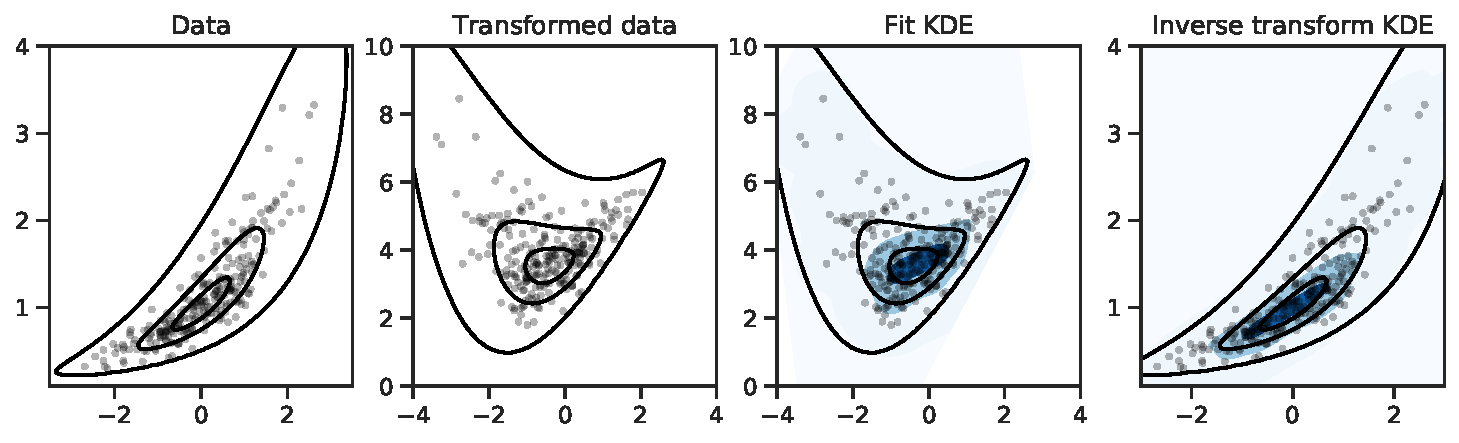
\includegraphics[width=0.9\textwidth]{figures/snemo_kde/2d_rescaling_process.pdf}
    \caption{The process of transforming the data to use a kernel that captures the data covariance. The first panel shows the data in the original coordinates. The second panel shows the data after being transformed by the whitening transformation. The third panel shows the KDE fit with a normal Gaussian kernel, and the final panel shows the data and the KDE reprojected back into the original coordinates. In each panel, the same data points are shown as black dots. The true 1, 2, and 3 $\sigma$ contours are shown in differing shades of blue. The black lines indicate the 1, 2, and 3 $\sigma$ confidence intervals of the best-fit KDE.}
    \label{fig:2d_rescaling_process}
\end{figure}

\begin{figure}
    \centering
    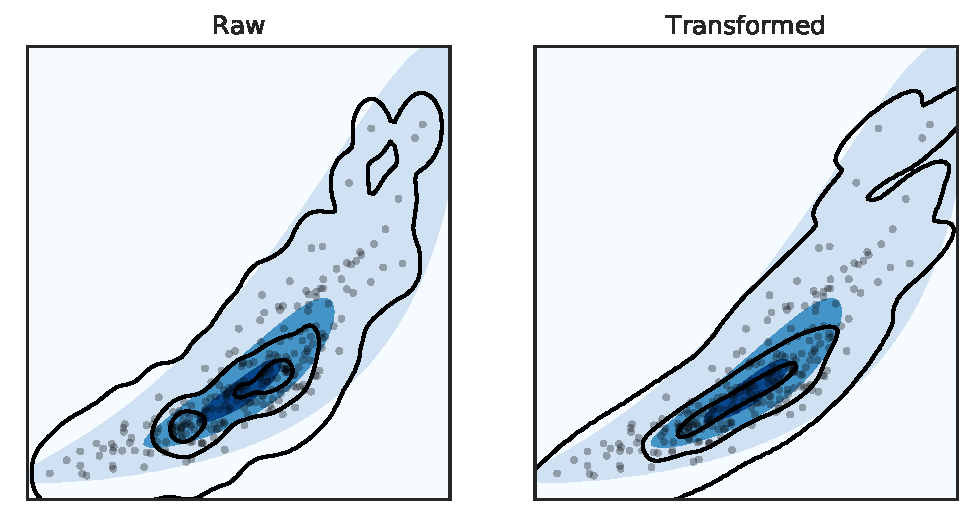
\includegraphics[width=0.9\textwidth]{figures/snemo_kde/2d_scatter.pdf}
    \caption{Comparison of the final KDE for our toy example using a) the best-fit Gaussian kernel with no covariance transformation and b) the best-fit Gaussian kernel with whitening applied. In both panels, the blue shading indicates the 1, 2, and 3 $\sigma$ contours of the true toy model distribution, and the black lines indicate similar contours for the kernel density estimates of the distribution.}
    \label{fig:2d_scatter_scaled}
\end{figure}

\section{Modeling the Data and Making Mock Observations}
\label{sec:making_mocks}
\subsection{Comparing Parameter Distributions}
We apply the multidimensional KDE fitting process laid out in the previous section to the spectral model parameter measurements found in Section \ref{sec:data}. Corner plots of the data points and similarly sized samples drawn from the resulting transformed KDE are shown in Figs. \ref{fig:salt2_sample}-\ref{fig:snemo15_sample}.

\begin{figure}
    \centering
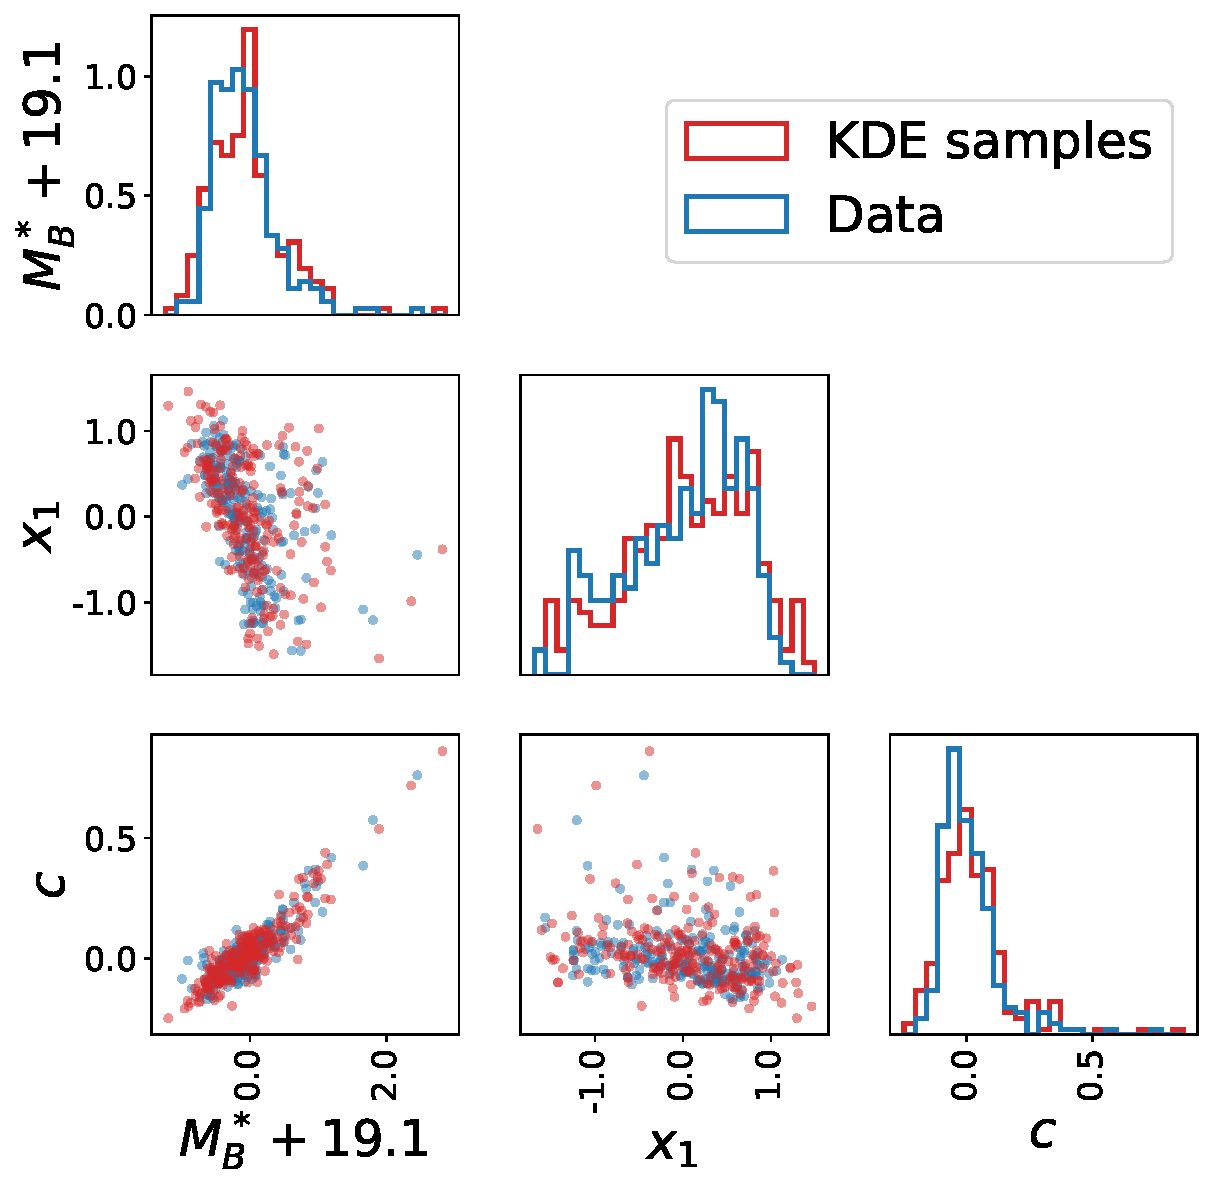
\includegraphics[width=0.9\textwidth]{figures/snemo_kde/salt2_corner.pdf}
    \caption{Corner plot showing the joint and marginal parameter distributions of the SALT2 parameters for the SNfactory data set (in blue), as well as the distribution of samples drawn from the KDE trained on these data (in red).}
    \label{fig:salt2_sample}
\end{figure}

\begin{figure}
    \centering
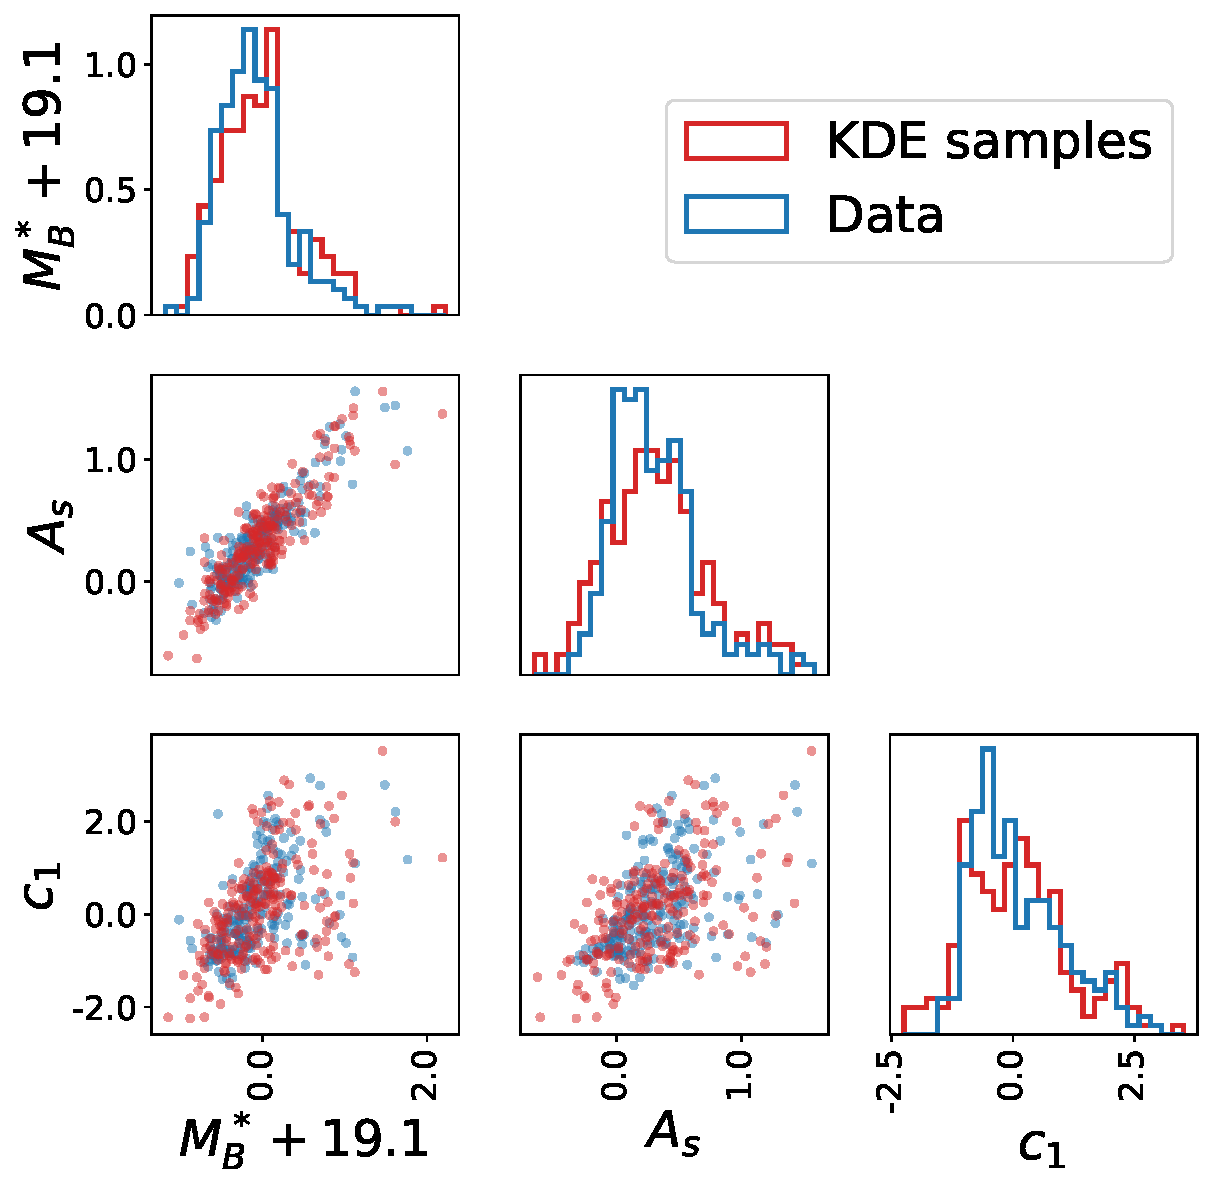
\includegraphics[width=0.9\textwidth]{figures/snemo_kde/snemo2_corner.pdf}
    \caption{Same as Fig. \ref{fig:salt2_sample}, but for SNEMO2}
    \label{fig:snemo2_sample}
\end{figure}

\begin{figure}
    \centering
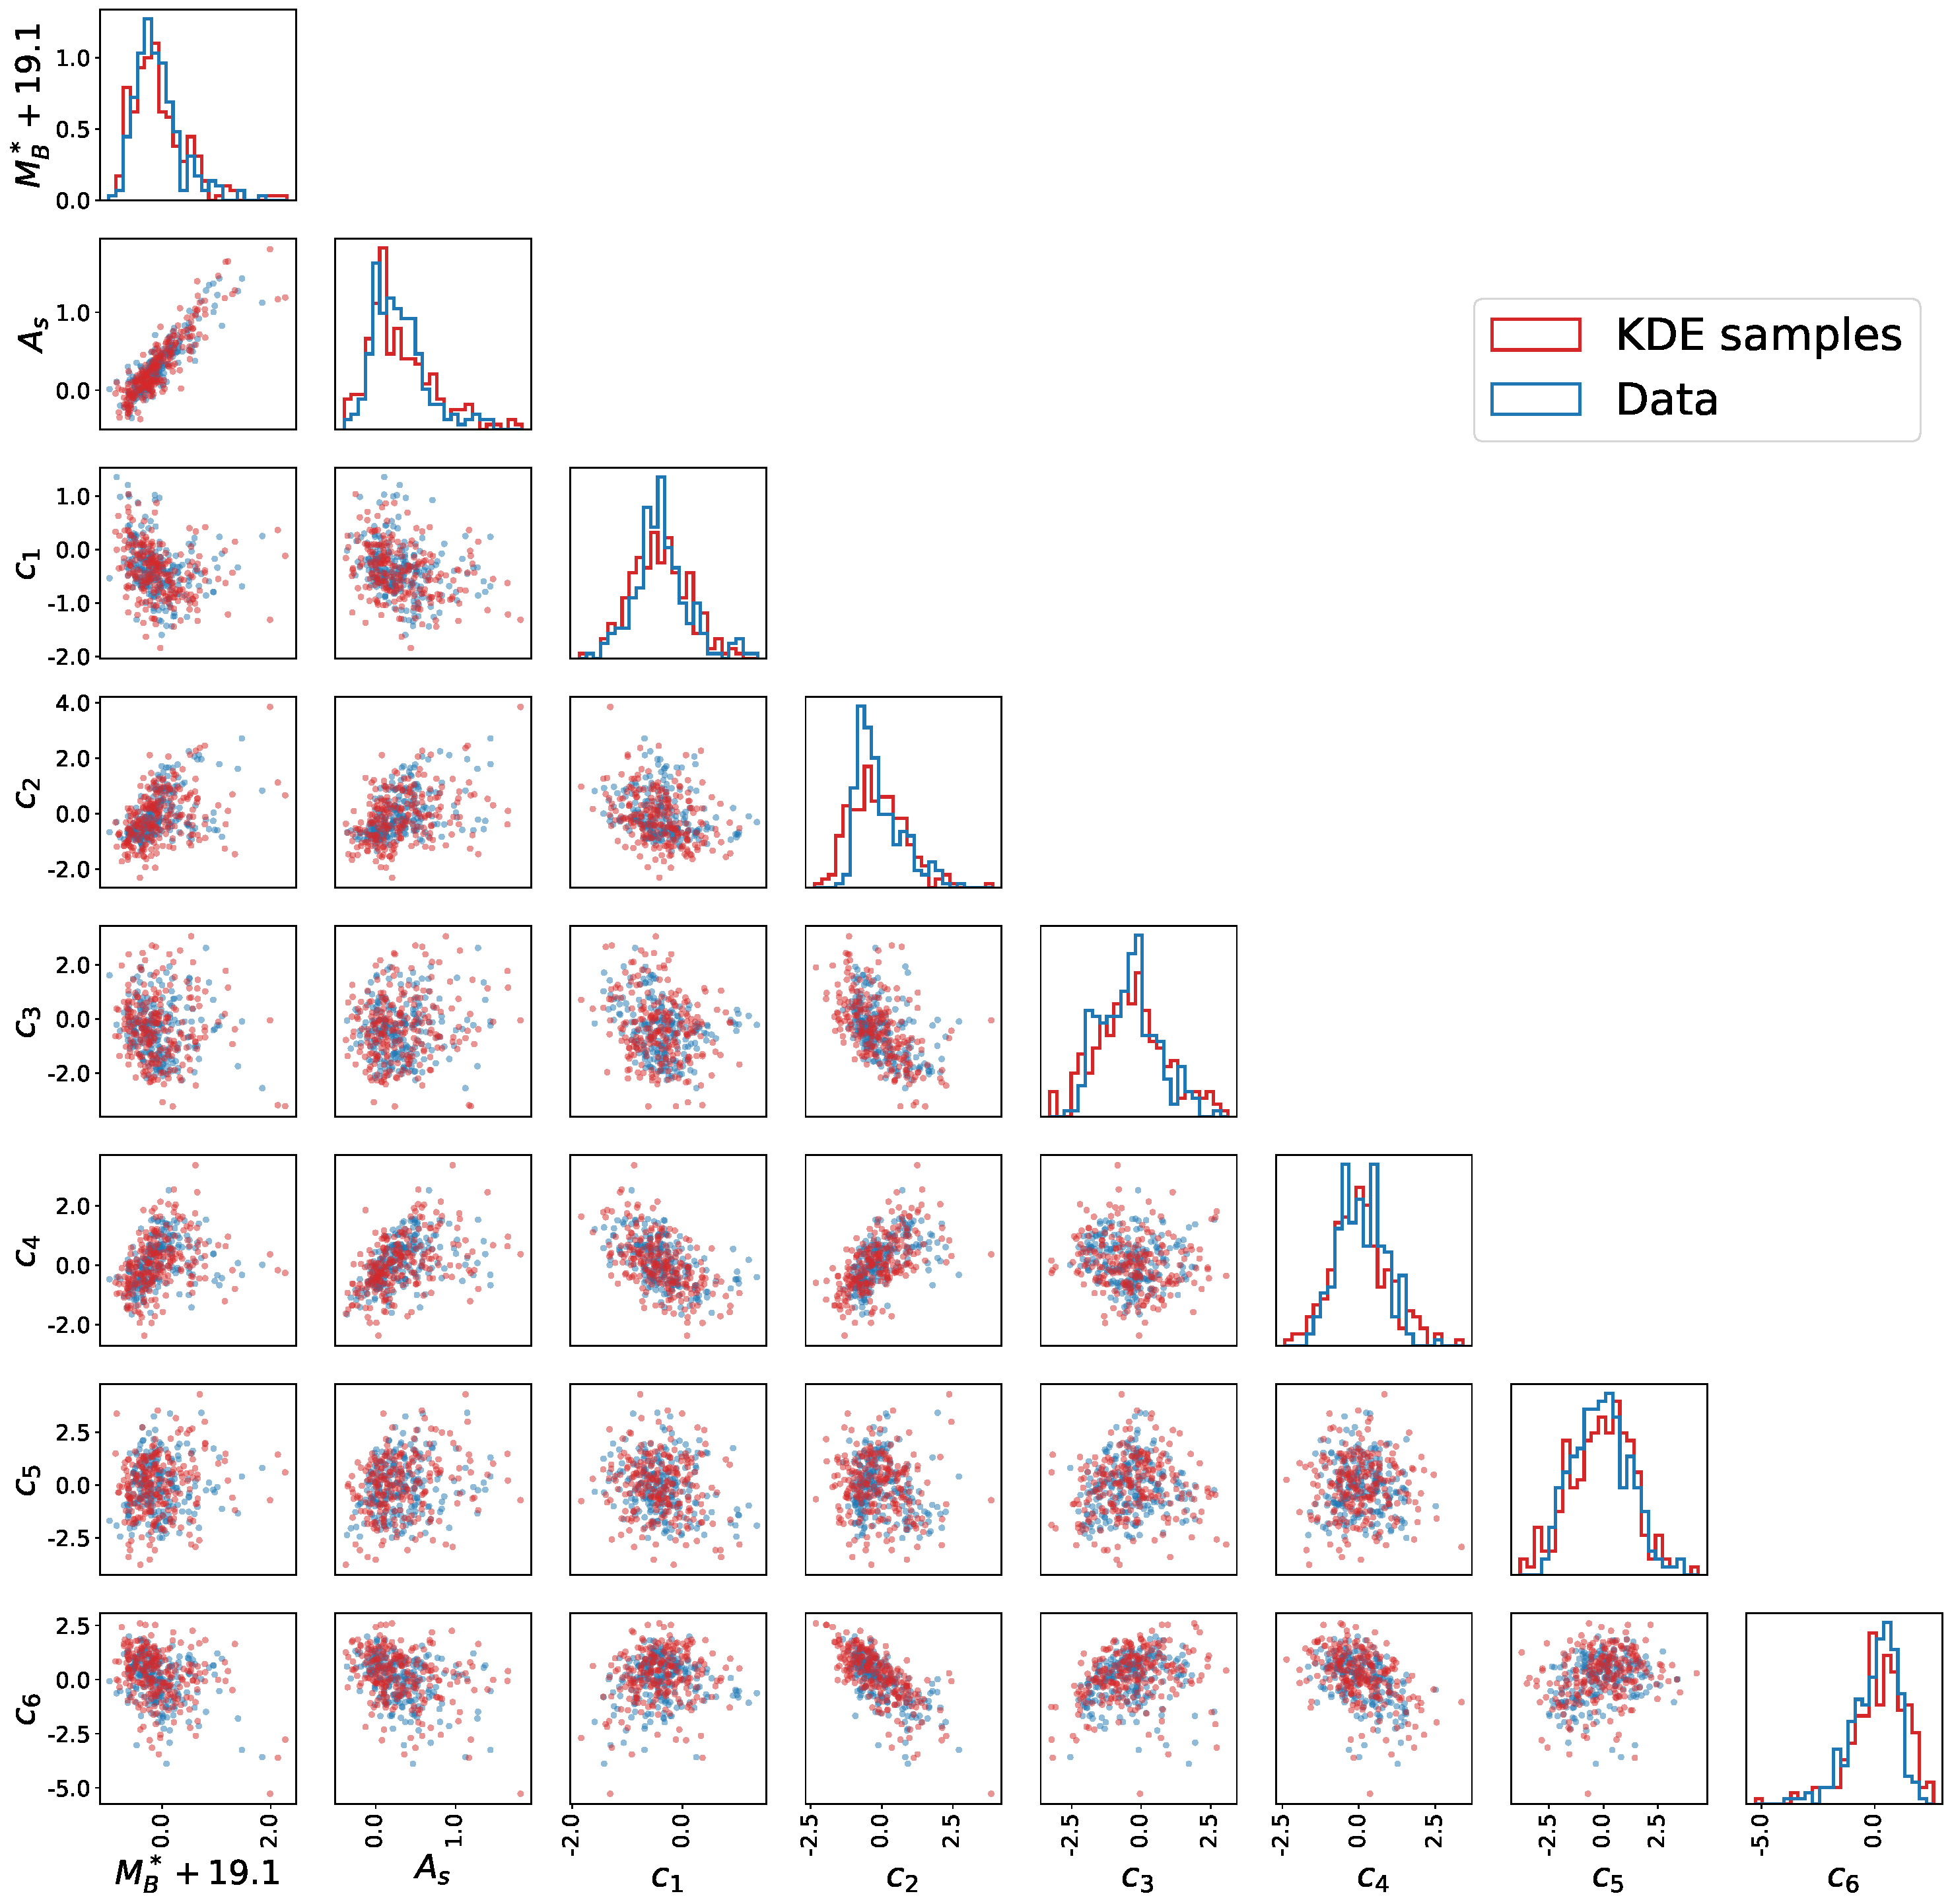
\includegraphics[width=0.9\textwidth]{figures/snemo_kde/snemo7_corner.pdf}
    \caption{Same as Fig. \ref{fig:salt2_sample}, but for SNEMO7}
    \label{fig:snemo7_sample}
\end{figure}

\begin{figure}
    \centering
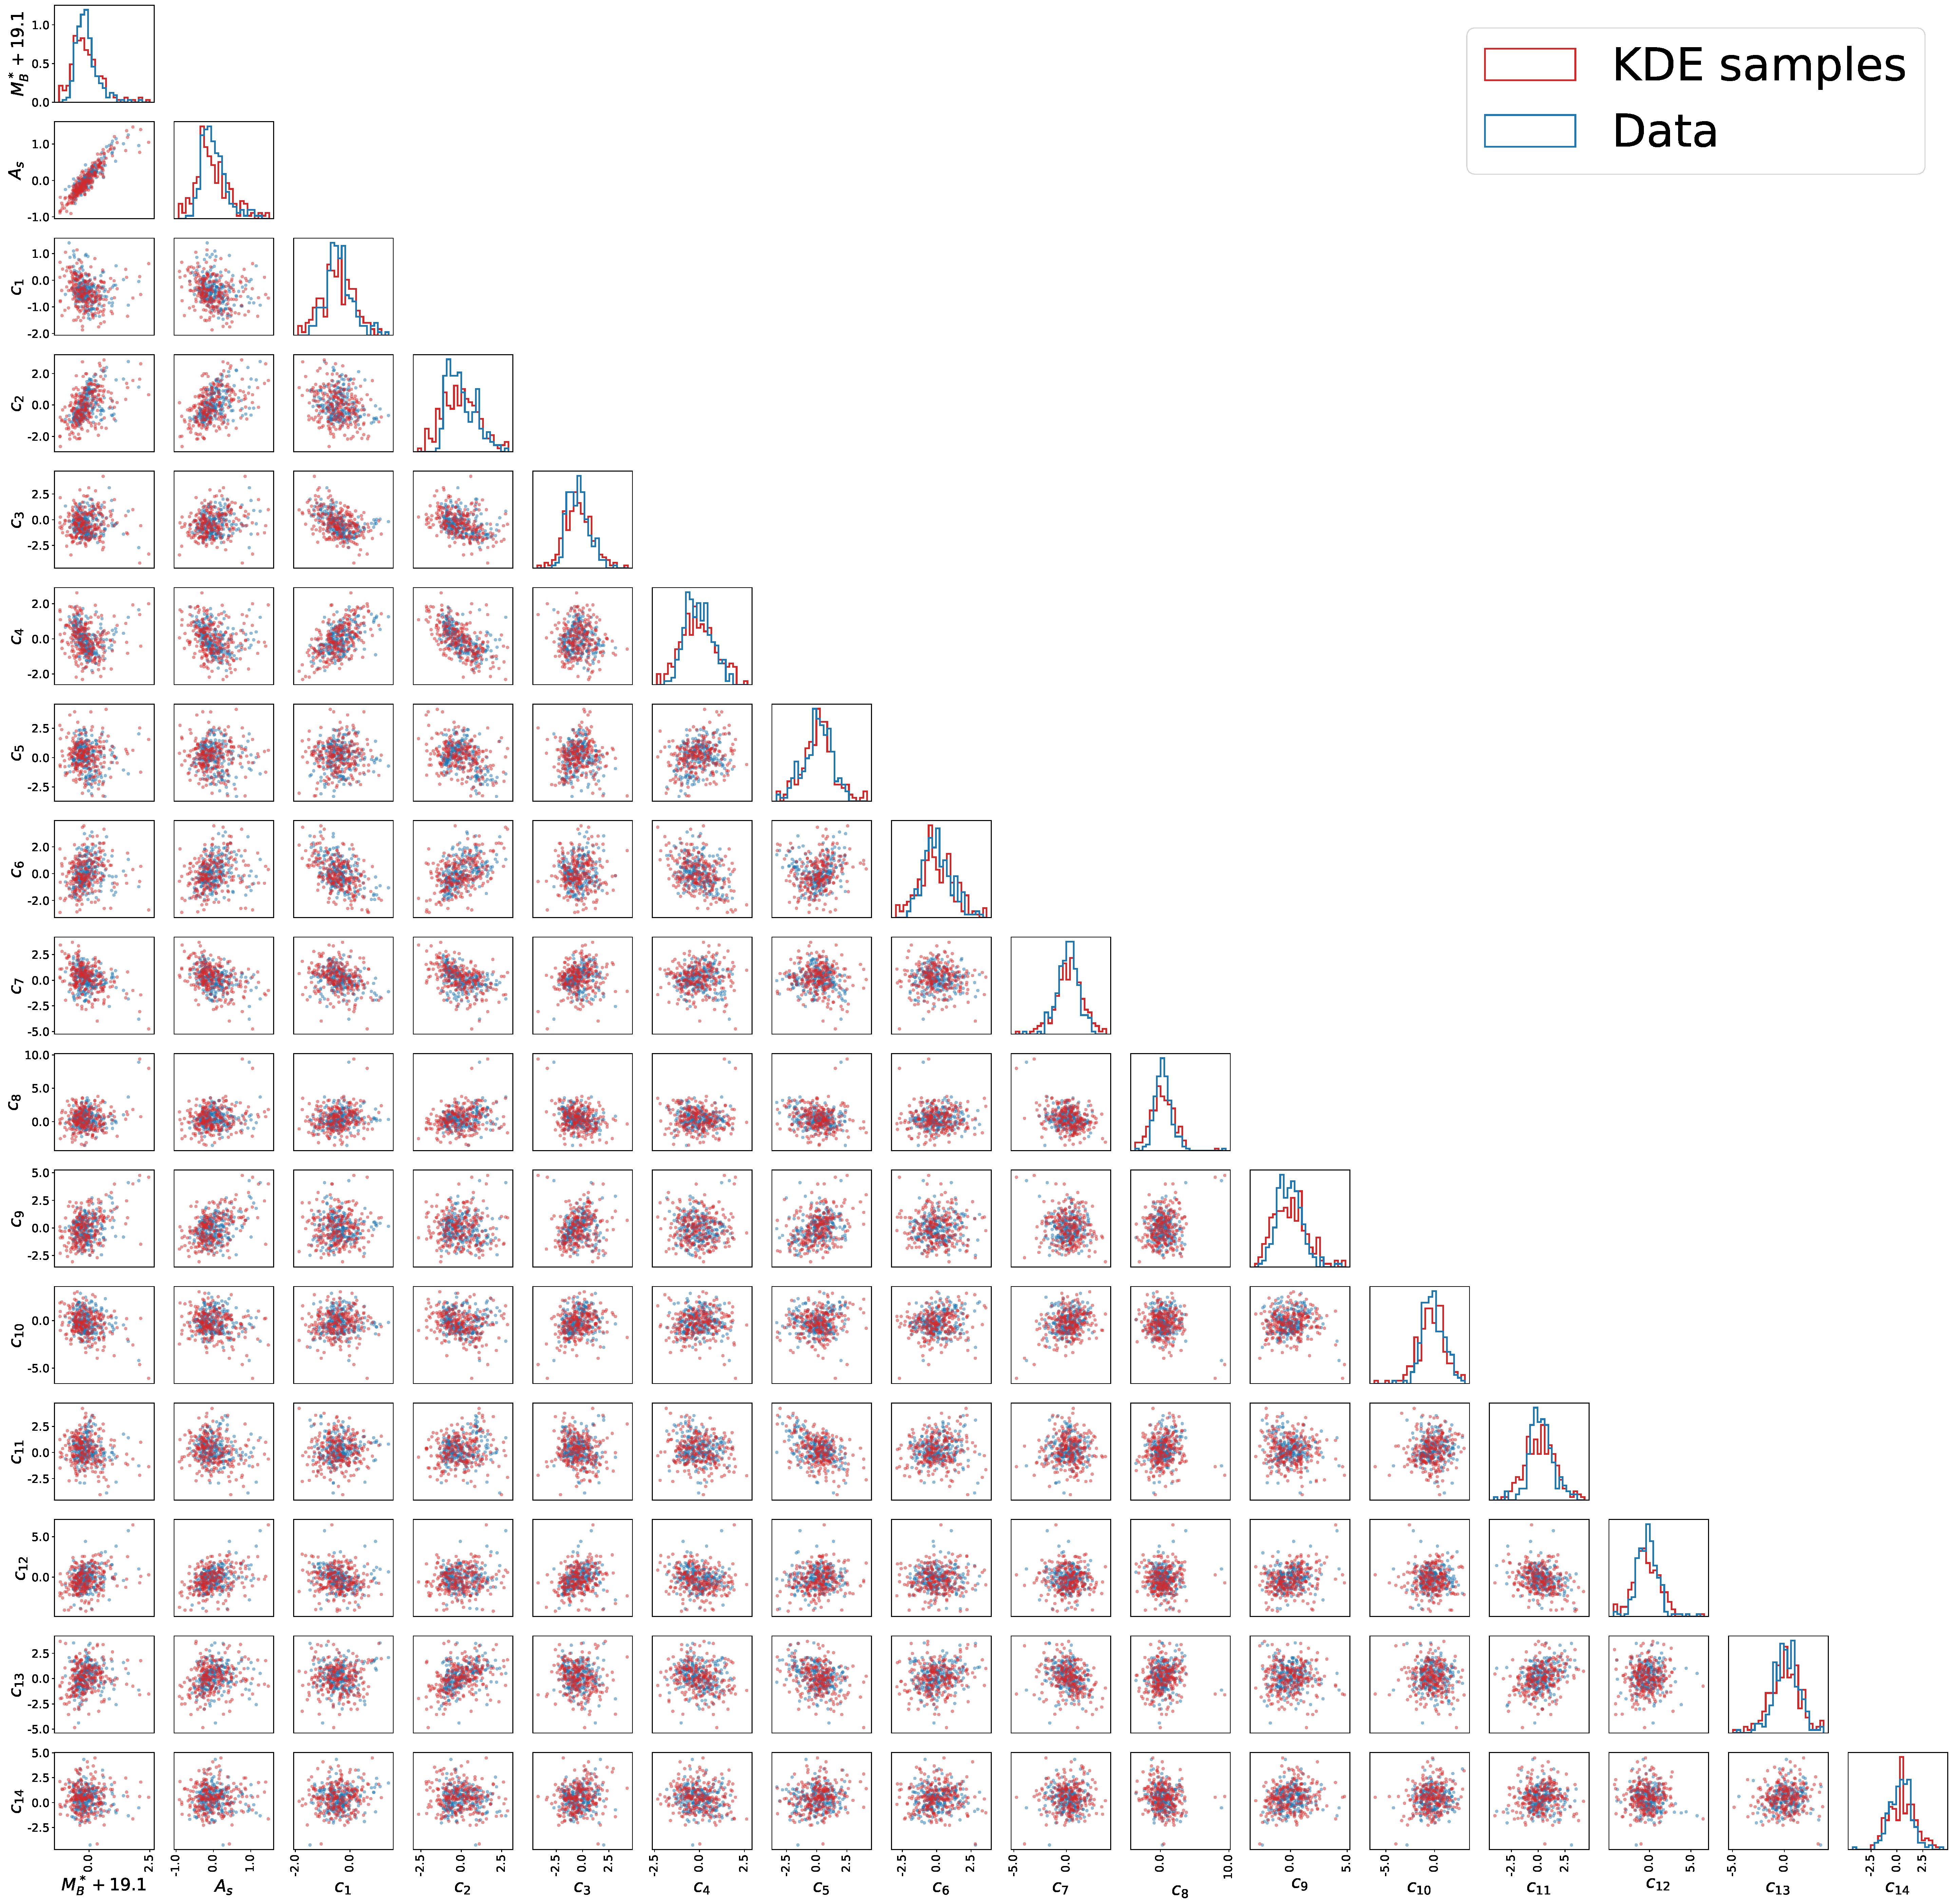
\includegraphics[width=0.9\textwidth]{figures/snemo_kde/snemo15_corner.pdf}
    \caption{Same as Fig. \ref{fig:salt2_sample}, but for SNEMO15}
    \label{fig:snemo15_sample}
\end{figure}

In order to quantify the advantage of using this kernel density estimate over a simpler model, like a multivariate Gaussian for example, we use the two-sample Cram\'{e}r distance \citep{Cramer1928} to measure the difference between the cumulative distribution function of the data and the estimated distributions from empirical cumulative distribution functions of the samples.
The Cram\'{e}r distance $\omega$ between a probability distribution with the empirical cumulative distribution function $F(x)$ and a second probability distribution with the empirical cumulative distribution function $G(x)$ is defined by
\begin{equation}
    \omega^2 = \displaystyle \int_\infty^\infty [F(x)-G(x)]^2 dx
\end{equation}
Smaller values indicate closer agreement between the two distributions.

This distance metric has the advantage over other more well-known test statistics (like the Kolmogorov-Smirnov statistic) of being sensitive to differences in the shape of distributions beyond just shifts in the mean or standard deviation, particularly in the tails of the distribution. This is ideal for our task because we want our parameter space estimates to match the true distribution across all portions of parameter space.

Calculating this distance in many dimensions is possible, but computationally difficult because of memory limitations in calculating large dimensional histograms. Therefore, we chose to compare each of the \emph{marginalized} distributions of each spectral model parameter. The Cram\'{e}r distances between the spectral model parameter marginal distributions from the best-fit KDE and from the data, as well as corresponding distances where a simple multivariate Gaussian replaces the KDE, are presented in Fig. \ref{fig:distances}.

\begin{figure}
    \centering
    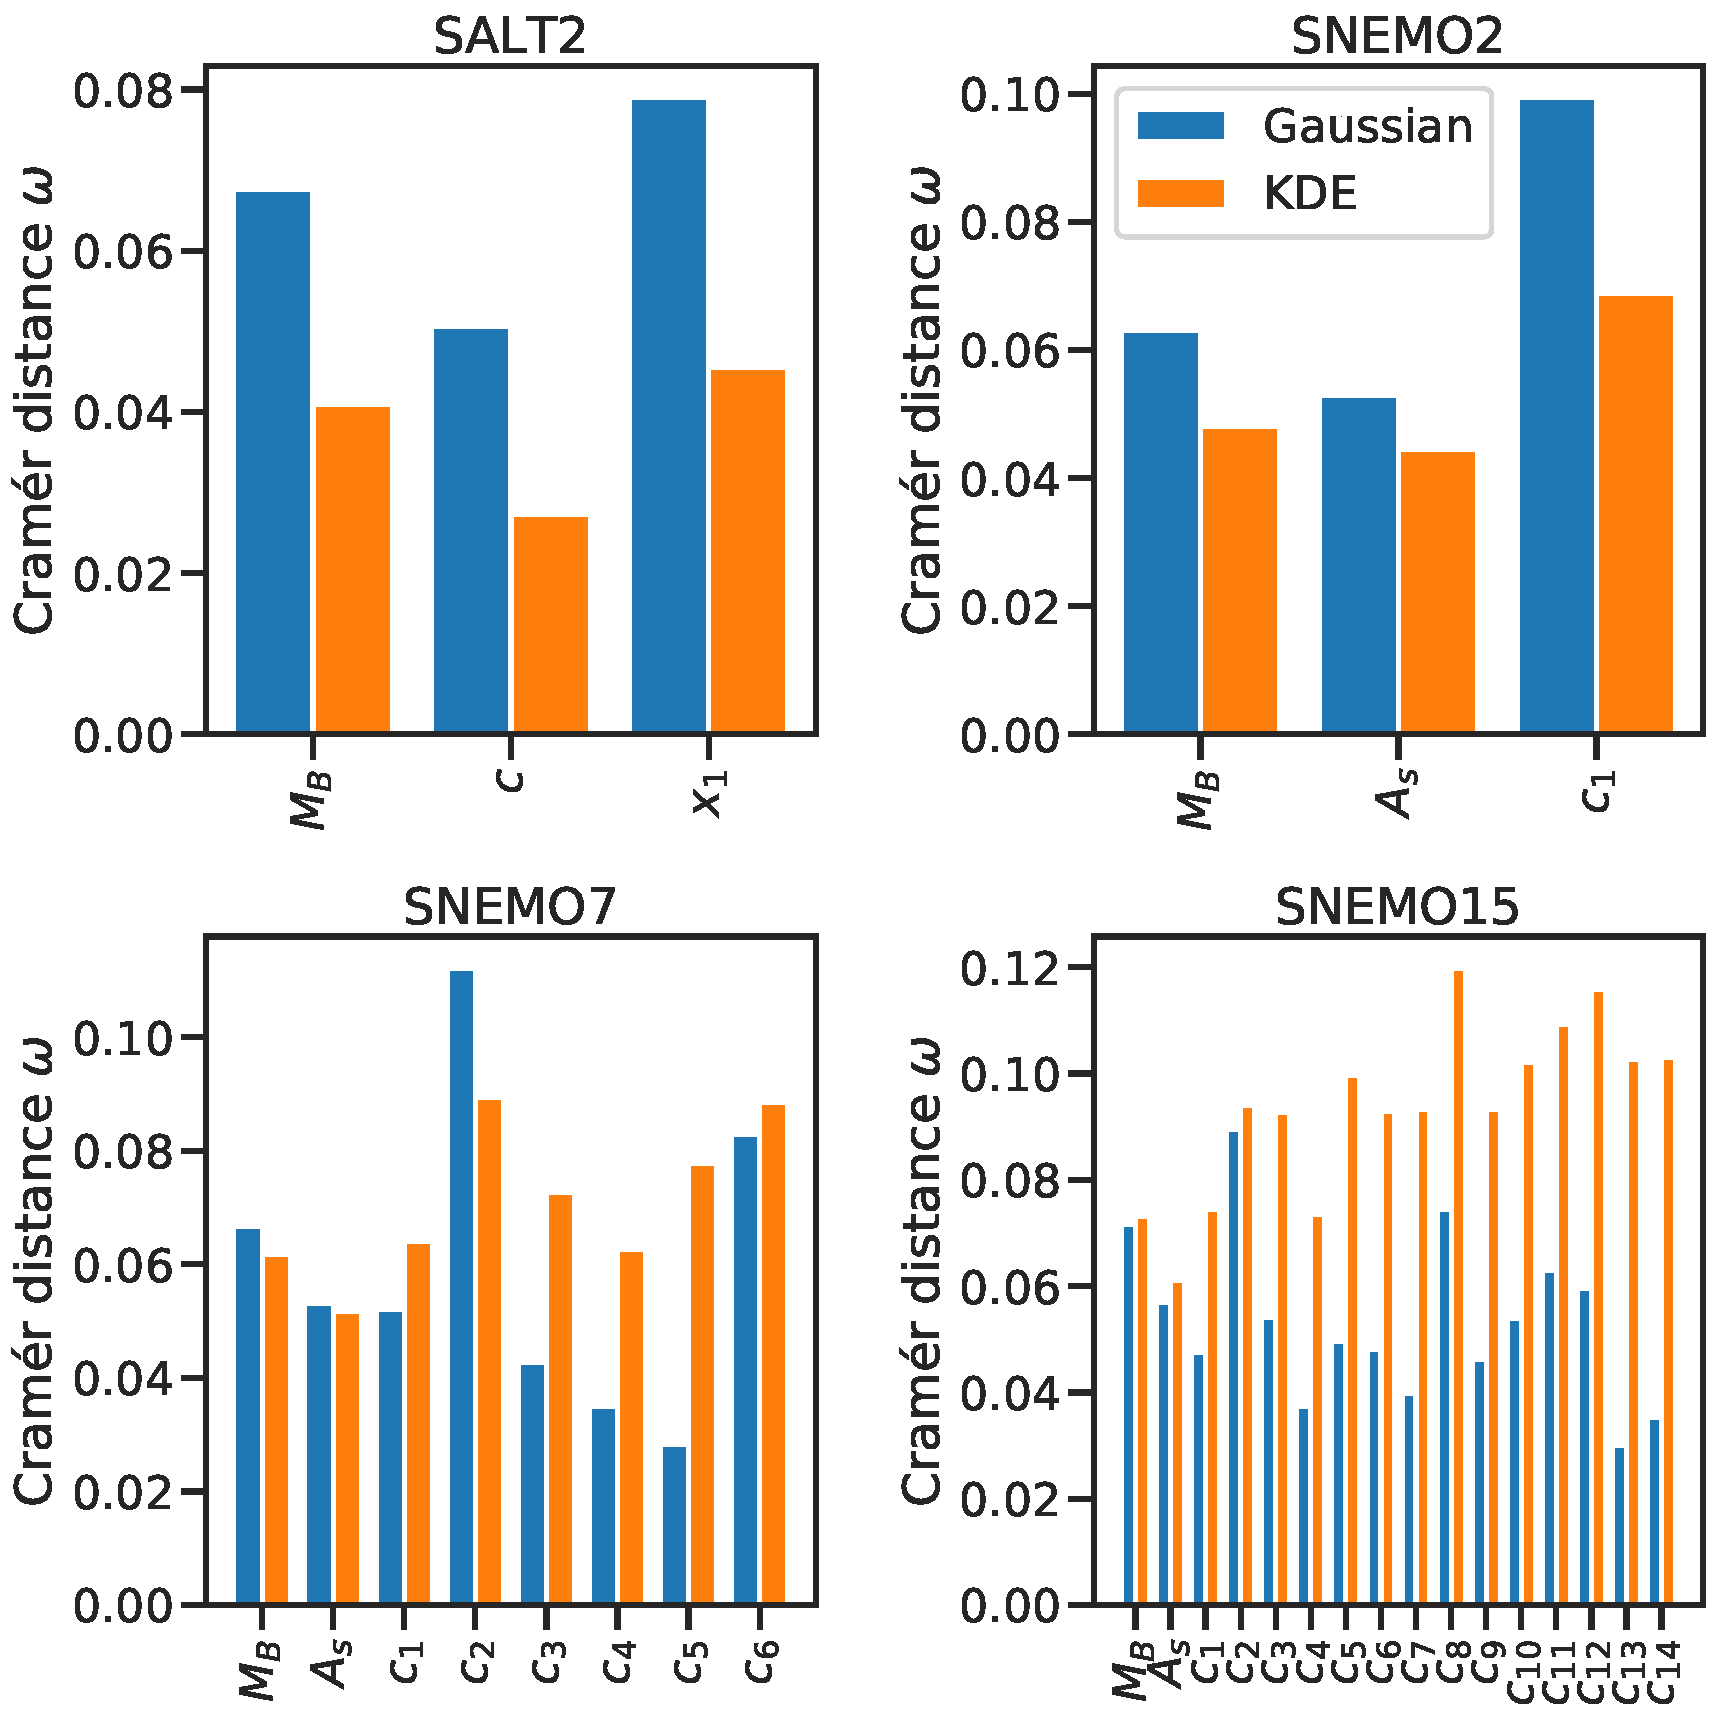
\includegraphics[width=0.9\textwidth]{figures/snemo_kde/cramer_distances_param_space.pdf}
    \caption{Cram\'{e}r distances between the empirical marginal distributions functions of the data sample and samples from a multivariate Gaussian (blue) and samples from the KDE (orange) for each parameter in each of the spectral models studied.}
    \label{fig:distances}
\end{figure}

In the lower-dimensional models (SNEMO2 and SALT2), the marginal distributions of the parameters found with the KDEs match those from the data much better than those drawn from a simple multivariate Gaussian. For SNEMO7, some of the marginalized parameter distributions, like $c_2$, are better described by the KDE than the Gaussian. Others, however, are better approximated by a Gaussian distribution. For SNEMO15, each of the marginalized parameter distributions are better modeled by Gaussians than they are by the marginalized KDEs. 

It is important to note that the metric we are using uses only the information from the marginalized probability. distributions, and therefore cannot account for skewness and non-Gaussianity in the joint probability distributions. As an example of this effect, we show the observed 2-dimensional joint distribution of SNEMO15 $A_s$ and $c_1$, along with contour plots of the same distribution given by the KDE and a multivariate Gaussian in Fig. \ref{fig:snemo15_joint_example}. While the Cram\'{e}r distance between the data and the marginalized KDE distributions of these two parameters is larger than the distance between the data and the marginalized Gaussian distribution, we see visually that the KDE seems to better capture the deviations from pure Gaussianity in the joint distributions, as evidenced by the closer agreement of the modes of the distributions and incorporation of larger tails in the distribution. Moreover, we will see in Section \ref{sec:spec_diversity} that using the KDE to model the spectral model parameter space allows us to capture a more realistic range of spectral feature measurements. The distances presented are meant to serve as a rough heuristic for the agreement between the distributions found by this technique and the data. A more detailed look, perhaps exploring the Cram\'{e}r distances in the two-dimensional distributions, is left to future work.

\begin{figure}
    \centering
    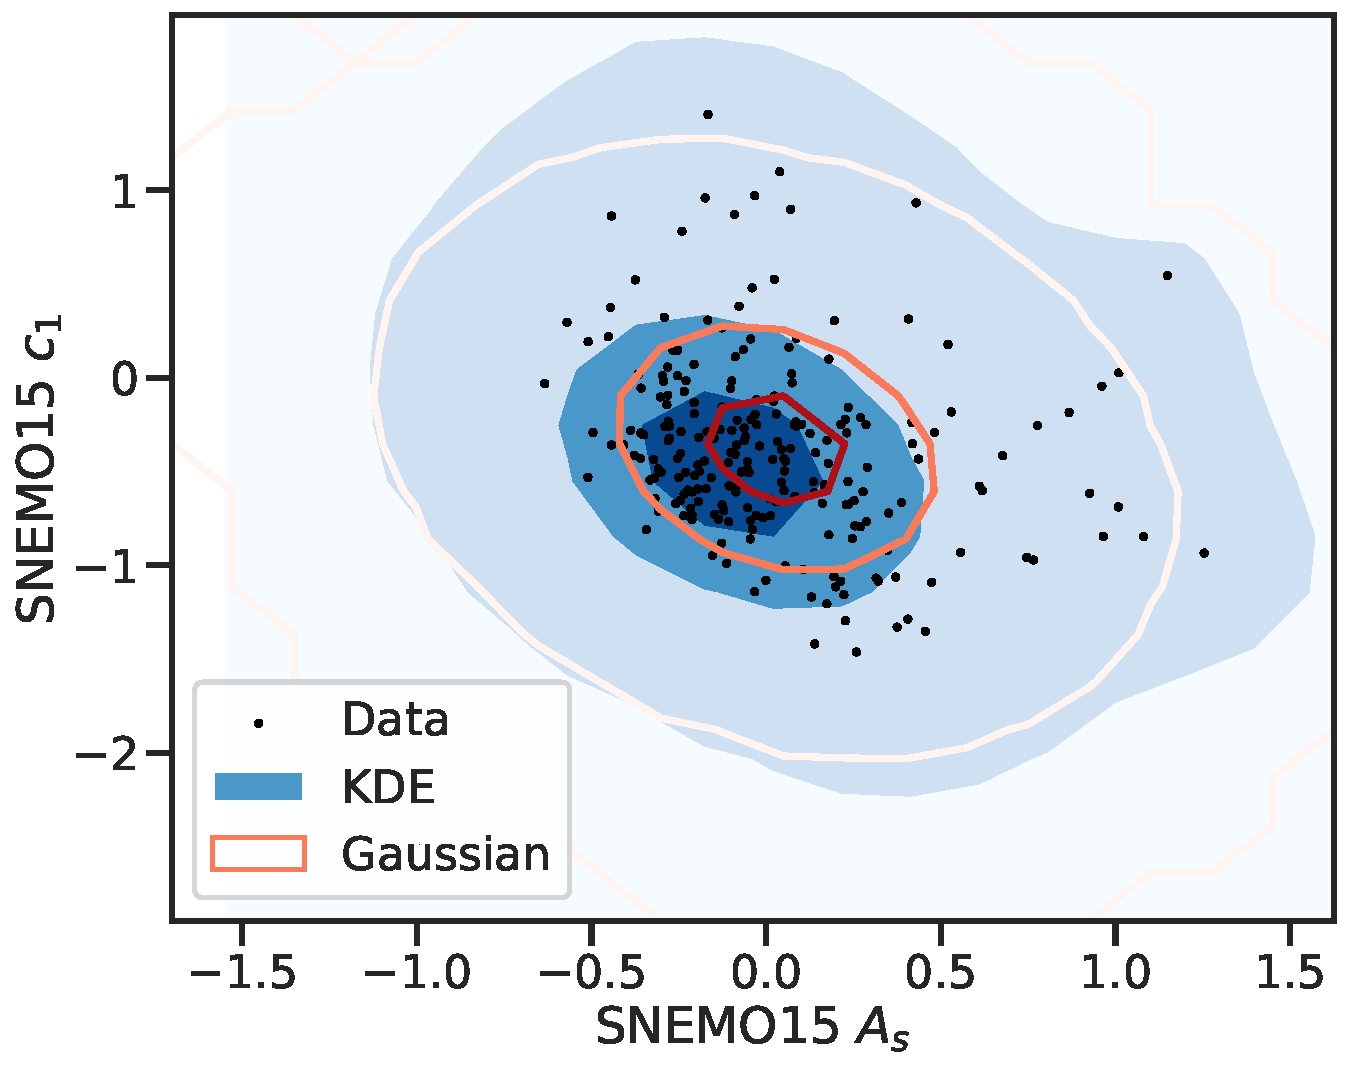
\includegraphics[width=0.9\textwidth]{figures/snemo_kde/snemo15_nongaussian_example.pdf}
    \caption{Comparison of the KDE estimate (blue filled contours representing the 68th, 95th, and 99th percentiles of samples drawn from the full 16-dimensional estimate) and multivariate Gaussian estimate (similarly spaced red line contours) of the joint probability distribution between SNEMO15 $A_s$ and $c_1$. While the Gaussian estimate shows a closer agreement in the marginal distribution of these parameters, according to the Cram\'{e}r distance (see Fig. \ref{fig:distances}), the KDE seems to allow a wider variety of values and better captures the skewness of this data because it is not constrained to match the Gaussian form.}
    \label{fig:snemo15_joint_example}
\end{figure}

\subsection{Generating Mock Observations}
With the modeled latent space in hand, we can easily obtain new SN Ia instances to use in further analyses by drawing from the underlying joint probability distribution, calculating the scaling coefficient $x_0$ or $c_0$, and plugging the resulting parameters into Eqn. \ref{eqn:salt_flux_model} or \ref{eqn:snemo_flux_model}. This process gives us a grid of flux values across the model wavelength range (3305-8685 \AA for the SNEMO models or 2000-9200 \AA for SALT2) and phase range (-10 to +40 rest-frame days after maximum brightness for the SNEMO models or -20 to +50 rest-frame days for SALT2).

As explained in Section \ref{sec:data}, we have modeled the absolute magnitude, rather than the redshift-dependent scaling parameters $x_0$ and $c_0$. To convert the $M_B^* + 19.1$ value to $x_0$ or $c_0$, we first choose a redshift $z$ for the supernova instance based on the needs of our analysis and calculate $m_B$, the peak apparent magnitude of an object at that redshift with $c_0=1$ and all of the remaining parameters set to values determined by the draw from the modeled distribution. We also calculate the desired apparent magnitude, $m_B^*$, by adding the distance modulus $\mu(z)$ from our fiducial cosmology to the apparent magnitude $M_B^*$ drawn from the modeled distribution. The final scale factor is then given by 
$$c_0 = 10^{-0.4(m_B^*-m_B)}.$$

Once we have our grid of flux values $f(\lambda, p)$, we can then easily synthesize spectroscopy or photometry of any resolution or signal-to-noise ratio using a tool like \verb|sncosmo|\footnote{\url{https://sncosmo.readthedocs.io/en/v2.1.x/}}. In Fig. \ref{fig:example_prism_spec}, we show spectra of an example object at redshift $z=0.775$ with intrinsic flux determined by a draw from the KDE model of the SNEMO15 model parameters, using the spectral resolution of the proposed Roman Space Telescope prism spectrograph and signal-to-noise equivalent to an exposure time of roughly one hour. Fig. \ref{fig:example_roman_lc} shows the same object but observed through photometry in the bandpasses proposed for the Roman Wide Field Instrument for a similar exposure time. 

\begin{figure}
    \centering
    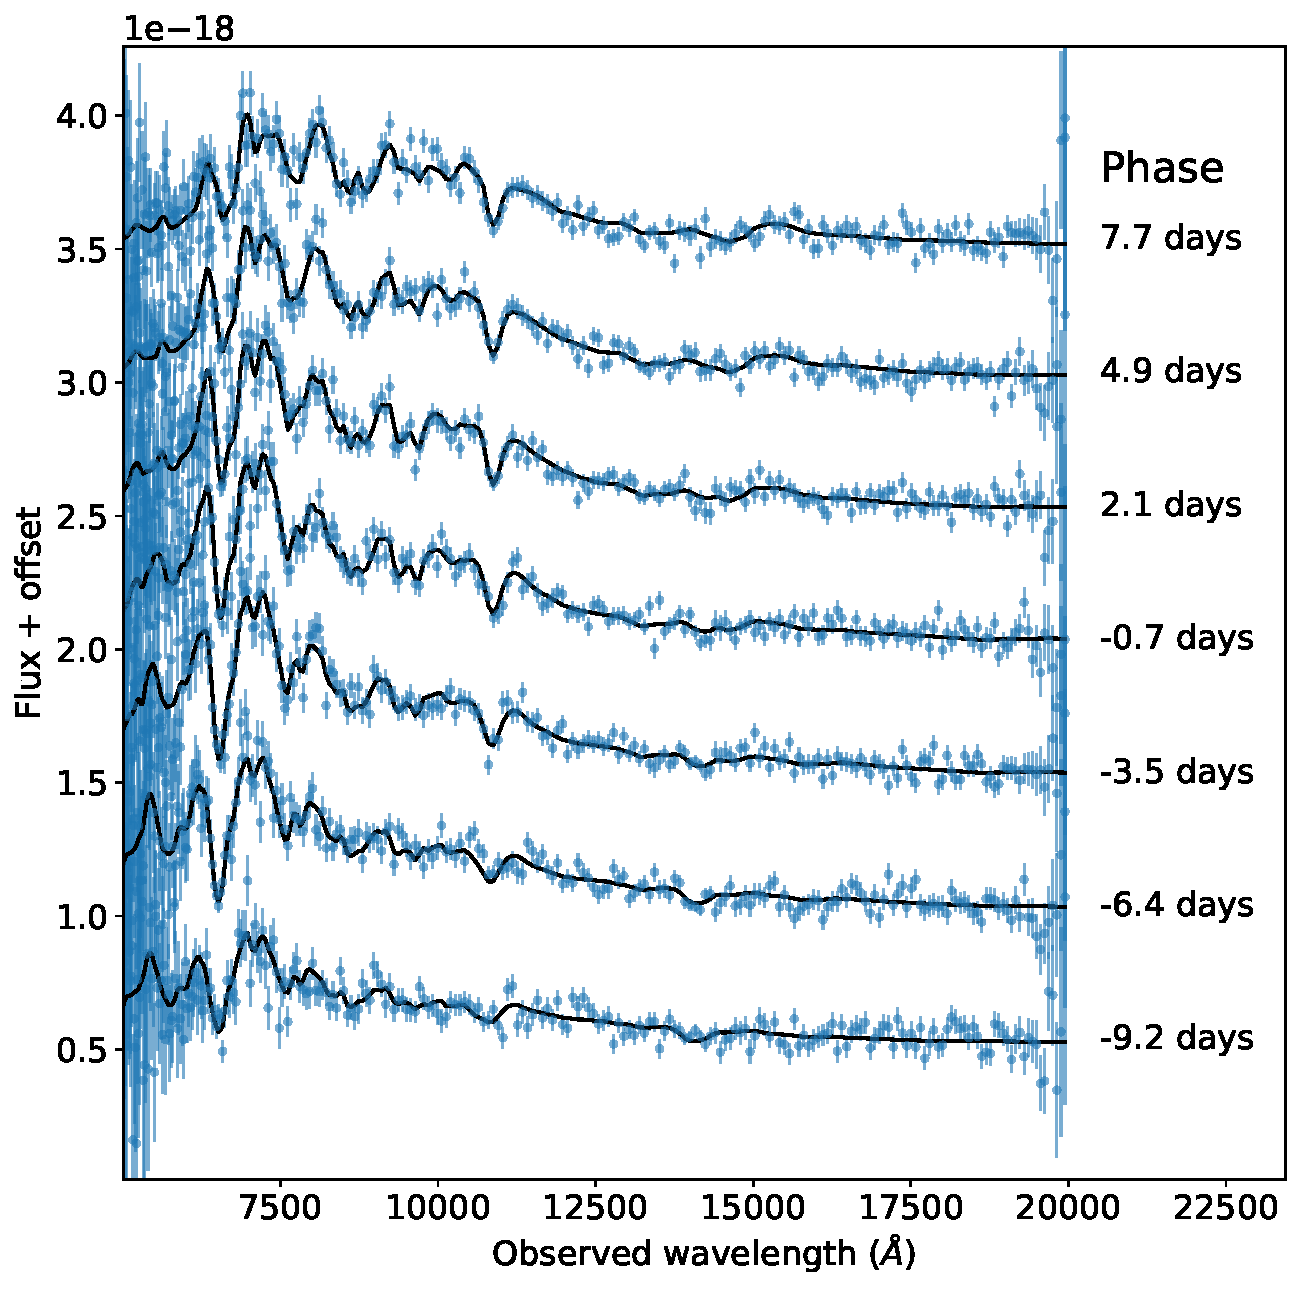
\includegraphics[width=0.9\textwidth]{figures/snemo_kde/example_roman_spec.pdf}
    \caption{A series of synthesized spectral observations at a range of phases for a single object at redshift $z=0.775$ generated from a random draw from the SNEMO15 KDE. The resolution matches the proposed design of the Roman Space Telescope prism spectrograph, and the signal-to-noise ratio representing the level that could be obtained with an hour of exposure time.}
    \label{fig:example_prism_spec}
\end{figure}

\begin{figure}
    \centering
    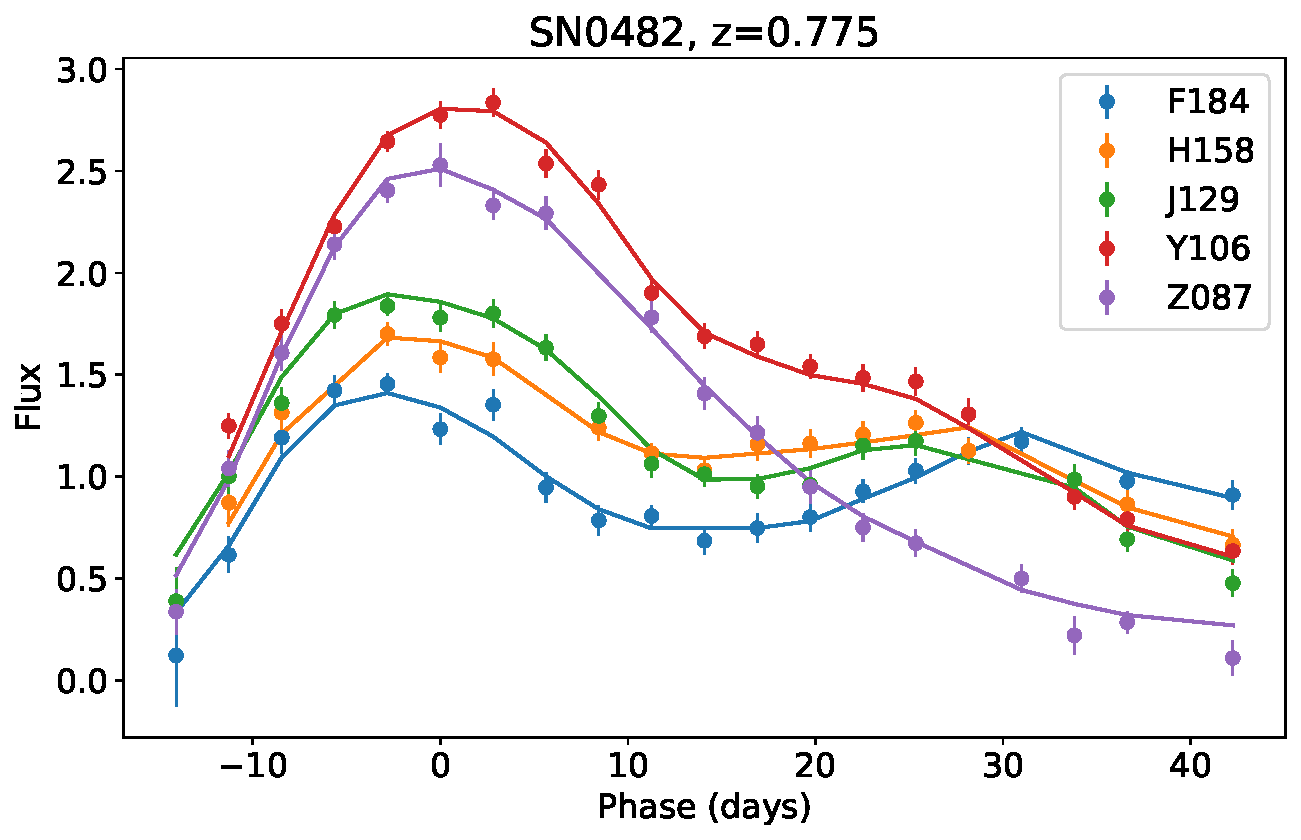
\includegraphics[width=0.9\textwidth]{figures/snemo_kde/example_roman_lc.pdf}
    \caption{Synthetic photometry of the same object shown in Fig. \ref{fig:example_prism_spec}, but observed photometrically in the Roman Wide Field Instrument bandpasses.}
    \label{fig:example_roman_lc}
\end{figure}

\section{Evaluating Spectral Diversity}
\label{sec:spec_diversity}
As another means of quantifying the usefulness of this tool, as well as a concrete example of the kind of analysis that is uniquely enabled by both a non-parametric model of spectral model parameters and the use of higher-dimensional spectral models (SNEMO7 and SNEMO15), we compare the distributions of several spectral features measured from the training spectra to the those obtained with data simulated by the techniques introduced in this work. The development of the SNEMO models was largely motivated by the recognition that spectral models like SALT2 do not capture the full range of spectral variation that is seen in Type Ia supernovae \citep{Saunders2018}. This study aims to quantify how well higher-dimensional linear models and non-parametric models of the latent parameter space of these linear models can capture the non-linear features that may provide a better understanding of supernova standardization and supernova physics.

We chose to focus on the velocities and pseudo-equivalent widths of the CaIIH\&K doublet, the SiII5972 line, and the SiII6355 line at maximum brightness. These spectral indicators are commonly used in studies aiming to improve the standardization of supernova brightnesses beyond light curve shape and color, or to quantitatively subclassify Type Ia supernovae in order to gain a better understanding of their physics. The ejecta velocities of SNe Ia, measured by the line velocities of SiII6355 and CaIIH\&K, have been shown to correlate with their intrinsic colors \citep{FoleyKasen2011, FSK2011, Foley2012, Mandel2014}. The width of the SiII6355 line shows a similar correlation \citep{FSK2011}. Evidence of a correlation between the velocity of the SiII6355 line and Hubble residuals has been shown directly in \cite{Siebert2020}. All of these relationships can lead to potential redshift-dependent distance bias if left uncorrected. An example subclassification scheme using these parameters is the Branch classification scheme \citep{Branch2006}, which arranges SNe Ia by the widths of their SiII5972 and SiII6355 lines, showing that there is a wide range in spectral feature behavior within the Ia class. 

To measure these features from real data (with associated flux noise), we first smooth the spectrum by convolving the observed flux $f(\lambda)$ with a Gaussian window weighted by the inverse of the flux variance, as is done in \cite{Blondin2006}, to get a smoothed spectrum $f_s(\lambda)$. Simulated spectra have no noise, so we do not smooth them. We do however interpolate both the smoothed, observed data and the simulated spectra onto a wavelength grid with 0.1 \AA resolution. For each feature region, we define a pseudo-continuum by identifying the local maxima $\lambda_{b}$ and $\lambda_{r}$ in the wavelength ranges blueward and redward of each feature described in Table \ref{tab:spec_feat_info} and calculating the line that connects these two points. We divide the flux by that line to obtain the pseudo-continuum-removed local feature spectrum $f_c(\lambda)$. The velocity of each line is determined by finding the wavelength of the minimum of the pseudo-continuum-removed local feature spectrum ($\lambda_\text{min}$) and using this value in the relativistic Doppler formula along with the rest-frame minimum wavelength $\lambda_0$ listed for each feature in Table \ref{tab:spec_feat_info}:
\begin{equation}
    \frac{v}{c} = \frac{\left(\lambda_\text{min}/\lambda_0\right)^2-1}{\left(\lambda_\text{min}/\lambda_0\right)^2+1}
    \label{eqn:rel_doppler}
\end{equation}
The pseudo-equivalent width is calculated by integrating
\begin{equation}
    \text{pEW} = \displaystyle\int_{\lambda_b}^{\lambda_r} \left[1-\frac{f_s(\lambda)}{f_c(\lambda)}\right] d\lambda
    \label{eqn:pew}
\end{equation}.

\begin{table}[ht!]
    \centering
    \begin{tabular}{|c|c|c|c|}\hline
    Feature name & $\lambda_b$ range (\AA) & $\lambda_r$ range (\AA) & $\lambda_0$ (\AA)\\\hline
    CaIIH\&K & 3504 - 3687 & 3887 - 3990 & 3945\\
    SiII5972 & 5550 - 5681 & 5850 - 6015 & 5972\\
    SiII6355 & 5850 - 6015 & 6250 - 6365 & 6355\\\hline
    \end{tabular}
    \caption{Extrema limits and rest-frame minimum wavelengths for the spectral indicators studied.}
    \label{tab:spec_feat_info}
\end{table}
These indicators were measured from the spectrum of each supernova in our data set that was closest to the SALT2-predicted time of B-band maximum brightness, $t_0$. To minimize the impact of phase evolution of the features, we remove from the analysis all objects that do not have a spectrum within $\pm 5$ rest-frame days of $t_0$. This leaves 213 supernovae. Code to perform these measurements is publicly available through the \verb|spectral_lines| package\footnote{\url{https://github.com/sam-dixon/spectral_lines}}.

\subsection{Comparing Features Measured from Data and from Best-fit Spectral Models}
We would like to separate our quantification of how well the spectral flux models themselves are able to capture the full distributions of spectral features from how closely samples generated from the KDE models of the spectral model parameters mimic the true distribution. To answer the first question, we make measurements of the spectral features from noiseless, at-max spectra synthesized directly from the best-fit spectral model parameters for each supernova and each spectral model (presented earlier in Table \ref{tab:snemo_coefs}). We will refer to these measurements as the model measurements.

Fig. \ref{fig:model_vSi_recovery} shows histograms of the residuals between these model-measured velocity of SiII6355 ($v_{SiII6355}$ and the data-measured velocity for each object in our data set. We can see that as the number of model components increases, the scatter on these residuals decreases, indicating that the increased flexibility of these higher-dimensional spectral models allows them to capture these spectral features. At SNEMO15, average difference between the model and data measurements of the velocity of this line is comparable in size to the typical measurement error of this feature.

\begin{figure}
    \centering
    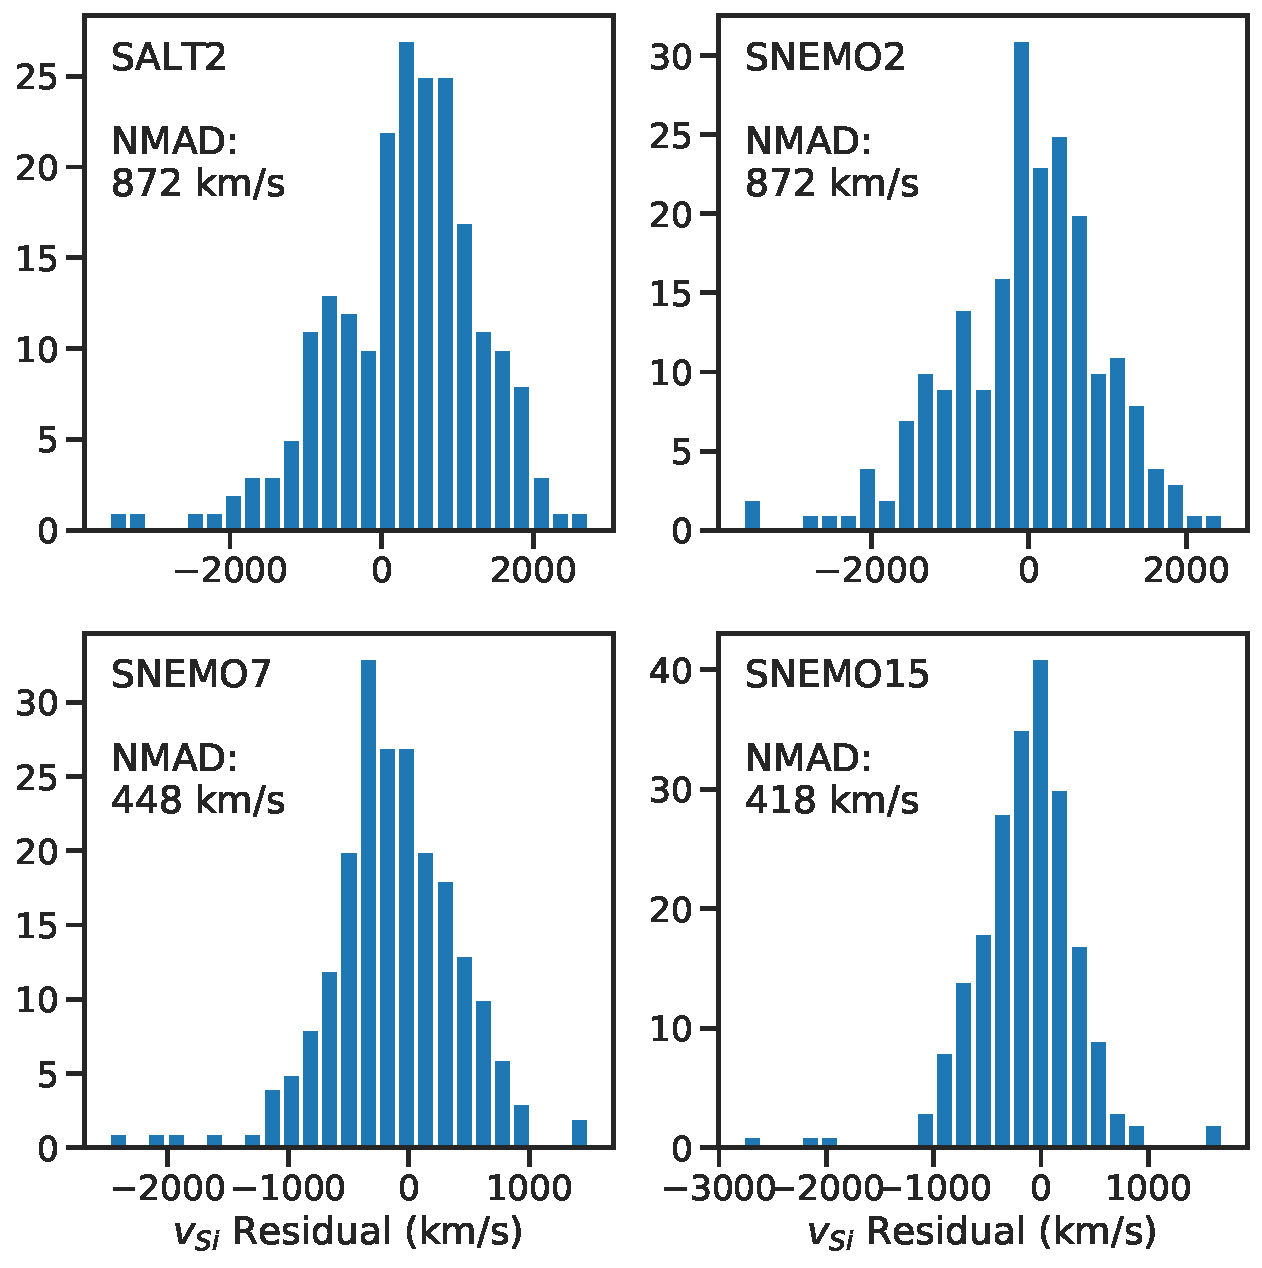
\includegraphics[width=0.9\textwidth]{figures/snemo_kde/model_vSi_recovery.pdf}
    \caption{Histograms of the residuals between the velocity of the SiII6355 line as measured from the data and as measured from the spectrum generated with the best-fit spectral model parameters. Lower dimensional models (SALT2 and SNEMO2) }
    \label{fig:model_vSi_recovery}
\end{figure}

This general trend is seen across all the spectral indicators studied, with the exception of the width of the SiII5972 line; we can see this in Fig. \ref{fig:model_spec_feat_recovery}, where we compare the normalized median absolute deviation ($\text{NMAD}(\bm{x})=1.4826\;\text{med}(|\bm{x}-\text{med}(\bm{x})|)$ of the residuals between model and data spectra for each spectral indicator across spectral models. It is not immediately obvious why the width of the SiII5972 line is captured nearly as well by SALT2 and SNEMO2 as it is by SNEMO15, but not captured by SNEMO7. It may be due to the fact that it is a relatively small feature, and therefore both more difficult to measure precisely on the data spectrum and poorly sampled in the SNEMO spectral eigenvectors. Regardless, we can still claim that SNEMO15 captures all of the spectral indicators studied the best.

\begin{figure}
    \centering
    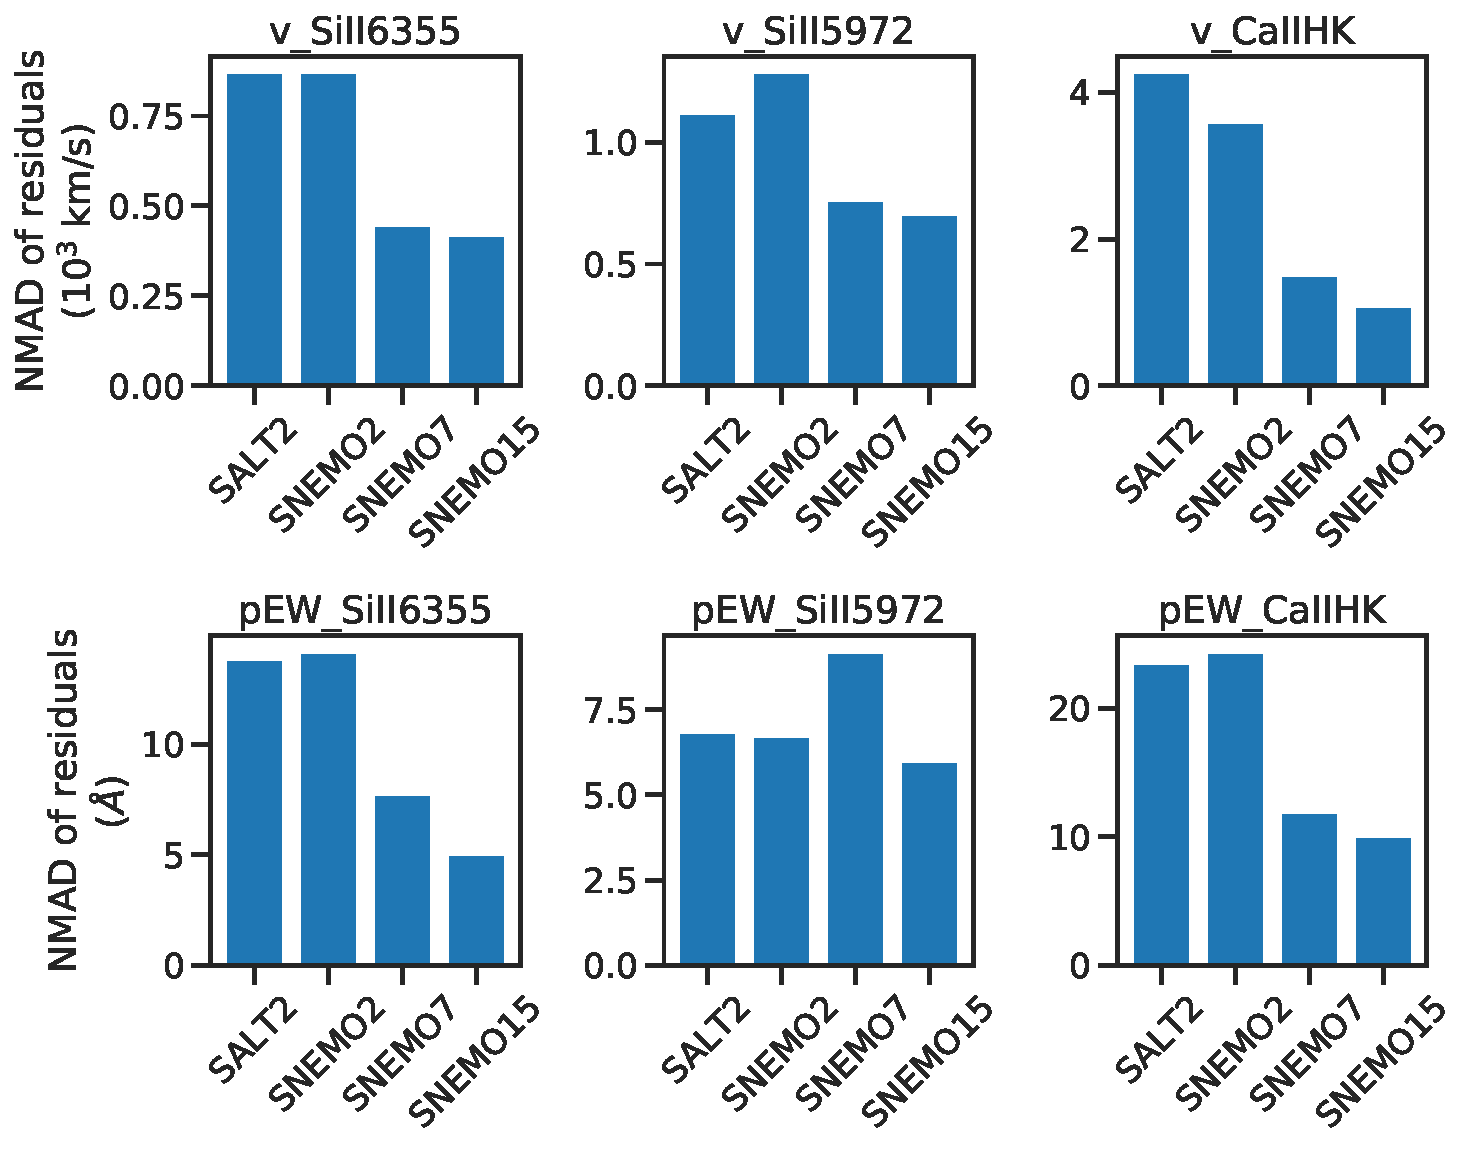
\includegraphics[width=0.9\textwidth]{figures/snemo_kde/model_spec_feat_recovery.pdf}
    \caption{Normalized median absolute deviation of residuals between spectral features measured from data spectra and from spectra generated from the best-fit spectral model. In general, spectral models with more parameters more closely capture the spectral feature measurements.}
    \label{fig:model_spec_feat_recovery}
\end{figure}

\subsection{Comparing Spectral Feature Distributions}
We can also compare the distributions of the spectral indicators seen in generated spectra that do not appear in our data set. To do so, we generate 1000 noiseless, at-max spectra from the KDE model of the spectral feature parameters and the multivariate Gaussian model as explained in Section \ref{sec:making_mocks}, and measure the six spectral indicators for each of these spectra.

The empirical cumulative distributions of the data and the KDE distributions for each of the spectral models are shown in Fig. \ref{fig:ecdf_kde}. A similar plot, but using the multivariate Gaussian model of the spectral model parameter space, is found in Fig. \ref{fig:ecdf_gauss}. These figures look quite similar, though we can pick out some differences (like the difference in the lower velocity portion of SNEMO15 distribution of $v_{SiII5972}$, or the differing relative fractions in each mode of the bimodal $v_{CaIIH\&K}$ distributions for SNEMO15).

\begin{figure}
    \centering
    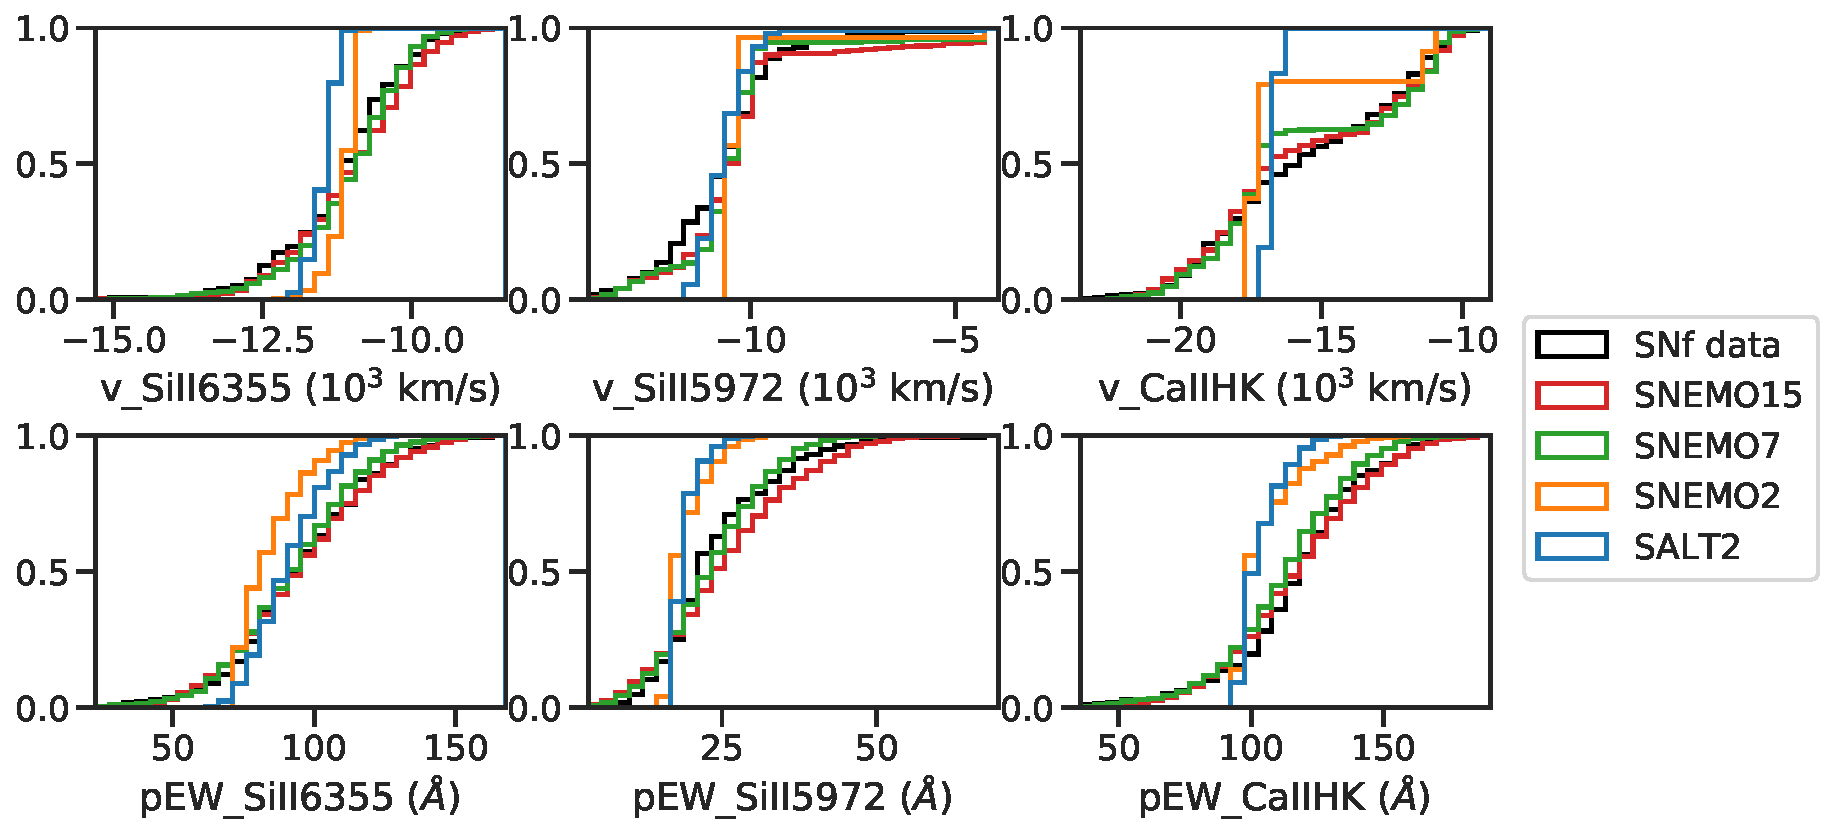
\includegraphics[width=0.9\textwidth]{figures/snemo_kde/ecdf_kde.pdf}
    \caption{Empirical cumulative distribution functions of each spectral indicator for the data set and samples from the kernel density estimate of the spectral model parameter spaces.}
    \label{fig:ecdf_kde}
\end{figure}

\begin{figure}
    \centering
    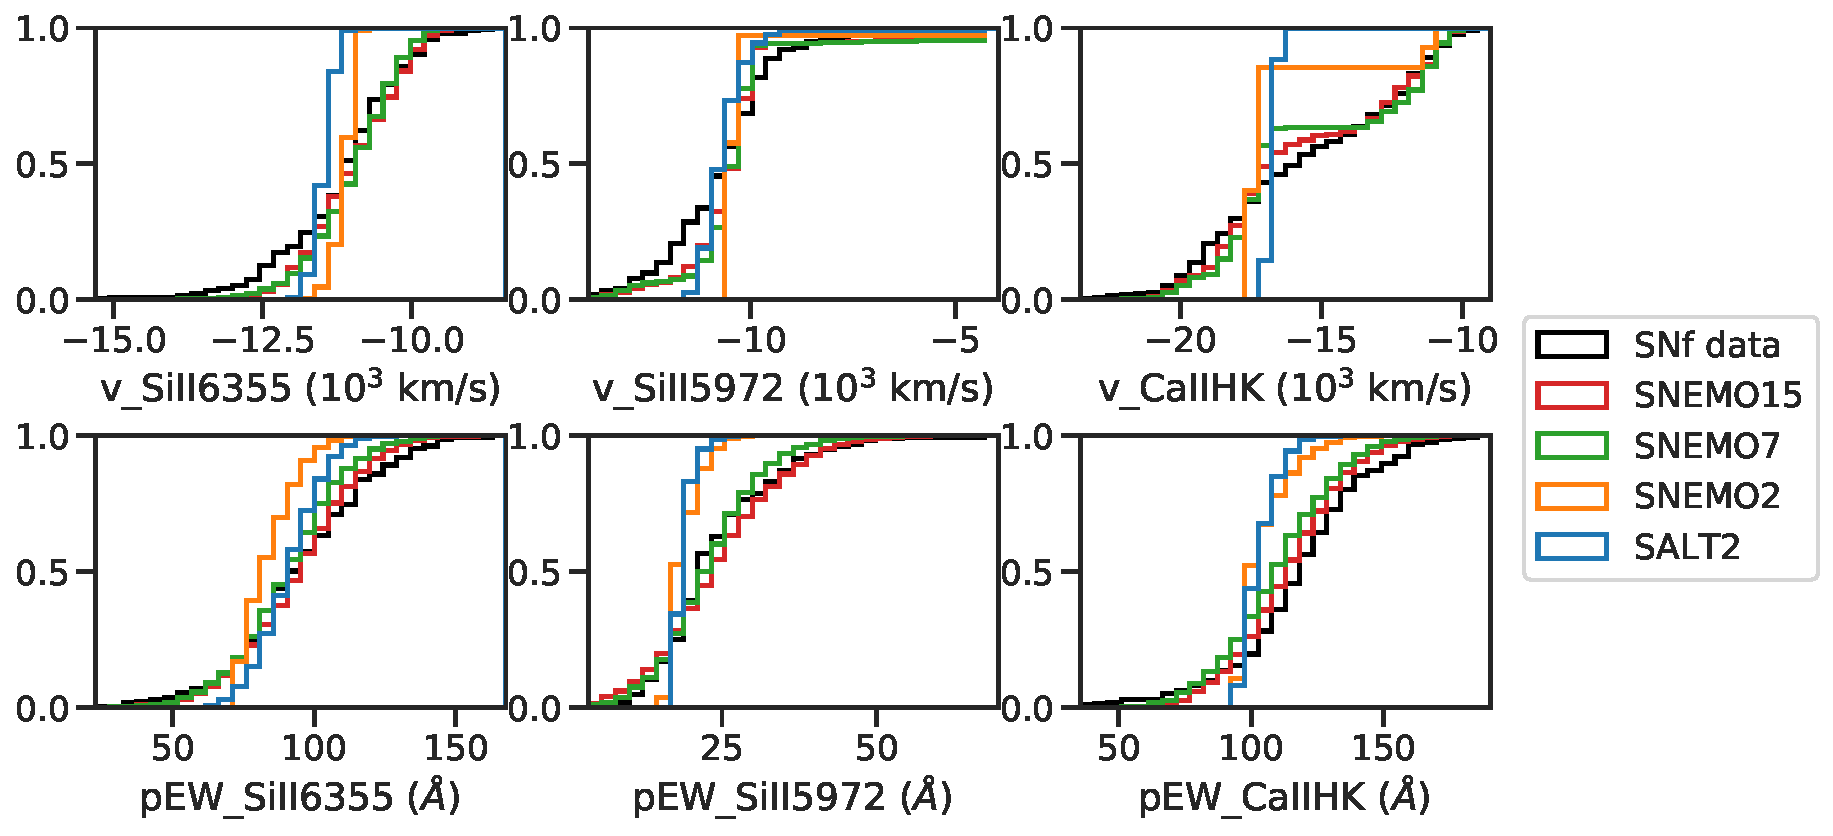
\includegraphics[width=0.9\textwidth]{figures/snemo_kde/ecdf_gauss.pdf}
    \caption{Same as Fig. \ref{fig:ecdf_kde}, but for samples from the multivariate Gaussian estimation of each of the spectral model parameter spaces.}
    \label{fig:ecdf_gauss}
\end{figure}

We can quantify these differences by calculating the Cram\'{e}r distances between the distribution of the data and the distribution of the samples for each feature. We get an estimate of the error on these distances with bootstrap resampling. The resulting distances for the KDE and Gaussian estimates are shown, along with the similarly calculated model to data distances, in Fig. \ref{fig:cramer_spec_feat}. We see a pattern similar to Fig. \ref{fig:model_spec_feat_recovery} in the spectral feature distribution similarity across models -- in every case, spectral models with more parameters have distributions of the spectral indicators that more closely resemble the data. Additionally, for each of the spectral models, the kernel density estimate of the model parameter distributions creates spectral feature distributions that are as or more similar to the true data distribution than the Gaussian estimates and the best-fit parameter spectra. Overall, using more flexible spectral models along with more flexible parameter space models allows for a generative model that can accurately reproduce the full range of spectral behavior for simulations.

\begin{figure}
    \centering
    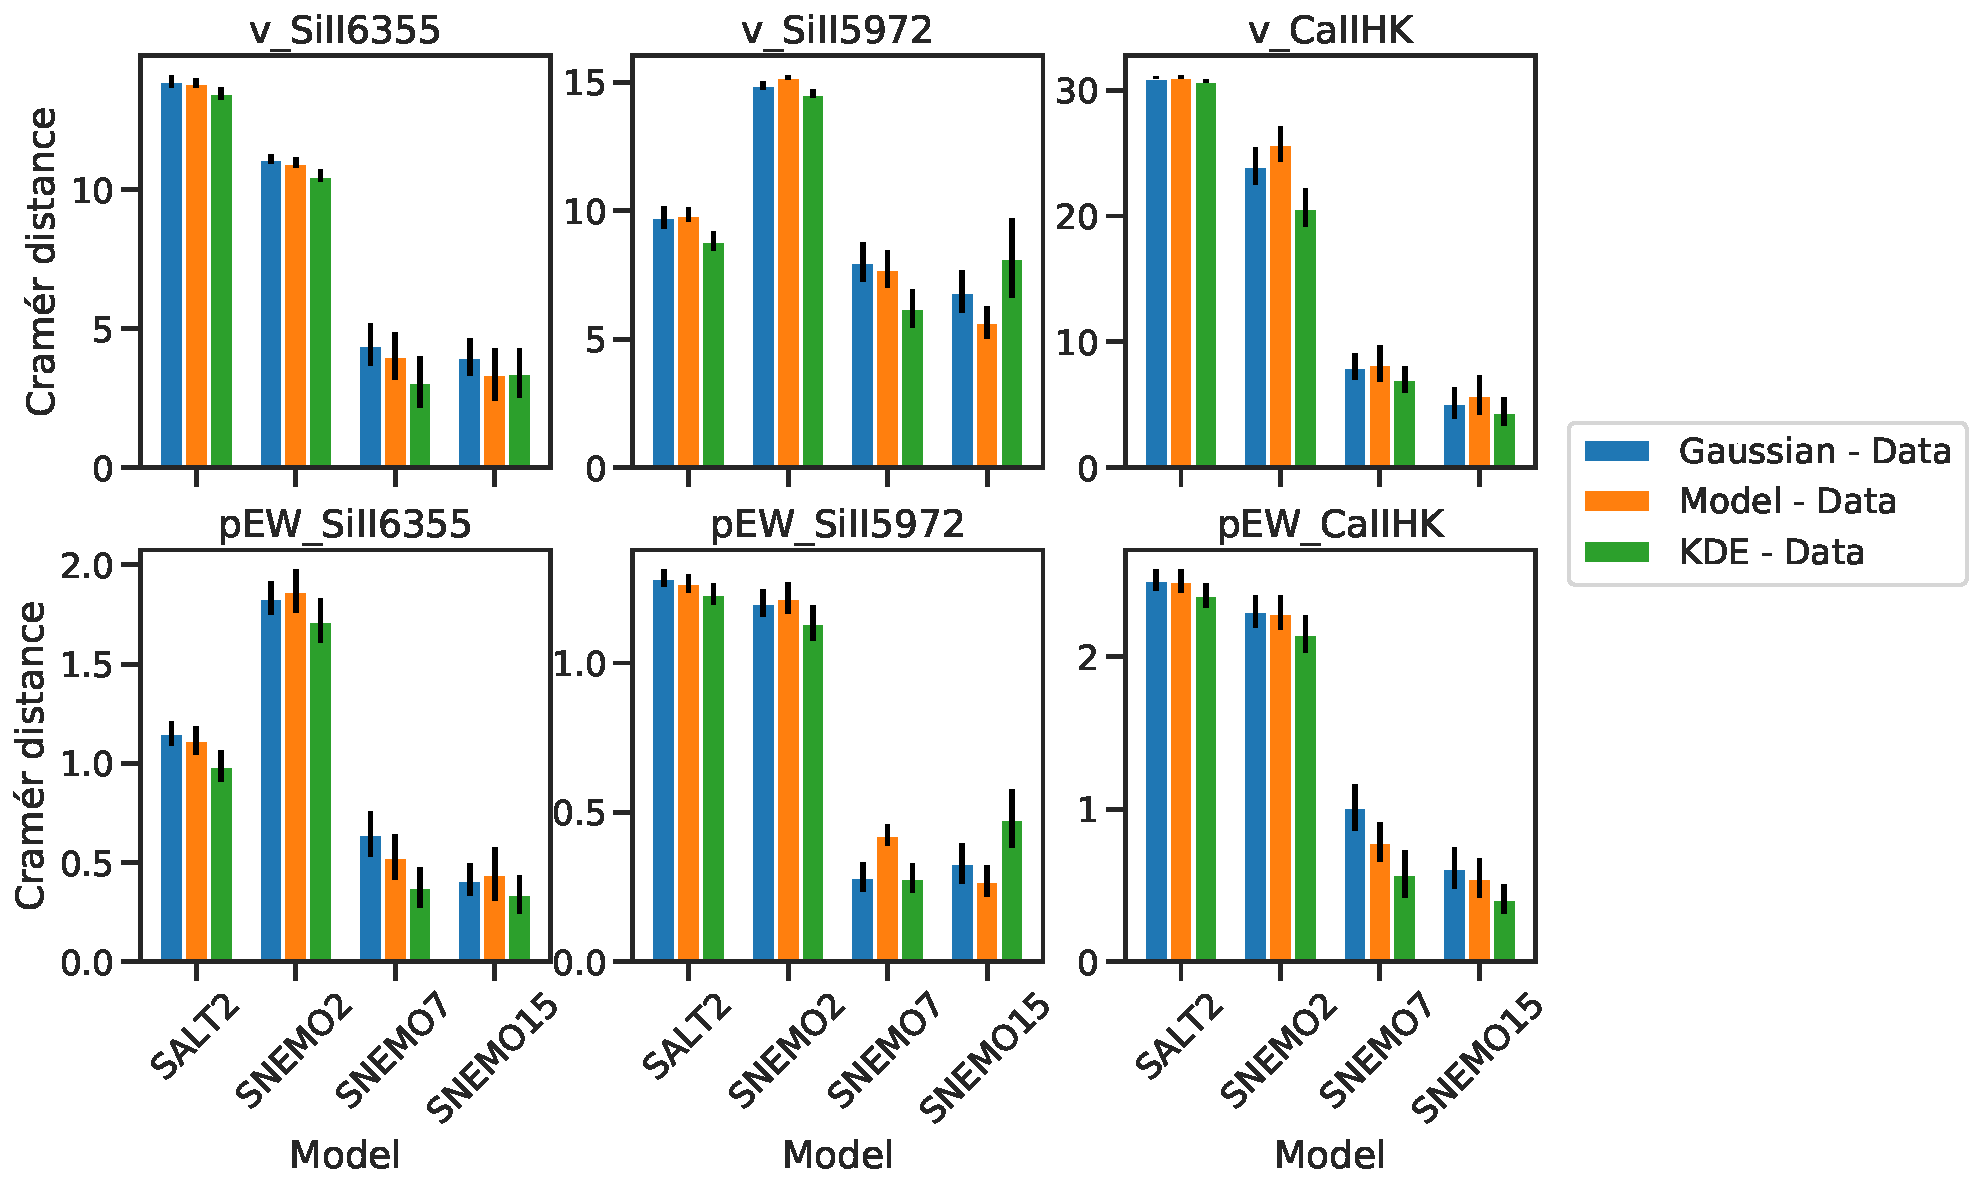
\includegraphics[width=0.9\textwidth]{figures/snemo_kde/cramer_distances_spec_feats.pdf}
    \caption{Cram\'{e}r distances between spectral indicator distributions for the SNfactory data and samples from the KDE estimates of the SALT2 and SNEMO parameter distributions, Gaussian estimates of the spectral model parameter distributions, and the modeled at-max spectra for the training data.}
    \label{fig:cramer_spec_feat}
\end{figure}

\section{Conclusions}
\label{sec:conclusions}
We have presented flexible estimates of the joint probability distributions of model parameters for the SALT2 and the SNEMO models of \cite{Saunders2018}. These estimates can be used to generate synthetic spectra and photometry in simulations that exhibit more spectral diversity than current state-of-the-art simulation techniques. This increased variety makes possible a number of different analyses, from examining the robustness of the twinning technique presented in \cite{Fakhouri2015}, to evaluating spectral feature measurement techniques under different observing conditions. There are a number of spectral properties of Type Ia supernovae beyond the two-parameter light curve shape and color parameters that have been shown to ultimately effect our cosmological parameter measurements. This work presents a simulation tool that properly incorporates these variations, allowing us to properly understand their impacts for future cosmological surveys.

\section{Appendix: Finding a Whitening Matrix}
\label{app:whitening_matrix_proof}
A matrix $W$ that satisfies $W^\top W=\Sigma_X^{-1}$ is a whitening matrix, i.e. if $X$ is a data matrix with covariance $\Sigma_X$, then $Y=WX$ has covariance $\Sigma_Y=\mathbb{I}$.
\begin{align*}
    \textrm{cov}(Y) & = \textrm{cov}(WX)\\
    & = W\textrm{cov}(X)W^\top \\
    & = W\Sigma_X W^\top \\
    & = W(W^\top W)^{-1}W^\top \\
    & = WW^{-1}(W^\top)^{-1}W^\top = \mathbb{I}
\end{align*}

Because the covariance matrix is positive-definite and symmetric, we can diagonalize it, finding a decomposition
$$\Sigma_X = U\Lambda U^T$$
where $\Lambda$ is a diagonal matrix whose entries are the eigenvalues of the matrix and $U^\top U = UU^\top = \mathbb{I}$, where the columns of $U$ are the eigenvectors. Then,
$$\Sigma_X^{-1}=(U\Lambda U^\top)^{-1} = U\Lambda^{-1}U^\top = (\Lambda^{-1/2}U^\top)^\top(\Lambda^{-1/2}U^\top)$$
and thus $W = \Lambda^{-1/2}U^\top$ is a whitening transformation.

\chapter{Measuring Type Ia Supernova Spectral Features from Low-Resolution and Noisy Spectra Using SNEMO}

\section{}
\chapter{Biases from Multicollinearity and Non-Simultaneous Regression in Supernova Cosmology}

\newcommand{\sgn}{\text{sgn}}
\newcommand{\sigint}{\sigma_{\text{int}}}

\section{Introduction} \label{sec:intro}
Properties of Type Ia supernovae (SNe Ia) have been observed to be correlated with their absolute luminosities. Before accounting for these properties, the absolute brightnesses of typical SNe Ia vary by $\sim 0.4$ magnitudes. After accounting for correlations with the decay time of the light curve and the color of the object, their corrected absolute brightnesses are consistent to within $\sim 0.14$ mag \parencite{Phillips93, Hamuy96, Riess96, Perlmutter97}. These calibrated brightness estimates are powerful cosmological distance indicator, and when combined with redshift measurements, allow us to map out the expansion history of the Universe. This technique was instrumental in the discovery of the accelerating expansion of the Universe \parencite{Perlmutter99, Riess98}, and continues to serve as a powerful probe of the nature of the dark energy driving this acceleration.

A common analysis method for standardizing supernova brightnesses uses the SALT2 model \parencite{Guy07, Betoule14, Mosher14} to parametrize SN~Ia light curves. The model parameters represent an individual supernova's peak apparent brightness in the Bessell B-band ($m_B^*$), temporal width ($x_1$), and observed color ($c$). The distance modulus $\mu$ to each object $i$ at redshift $z_i$ is then modeled as a linear combination of these parameters:
\begin{equation}
    \mu_i(z_i) = m_{B\;i}^*(z_i) - M + \alpha x_{1\;i} - \beta c_i
\end{equation}
Typically, we would find the values of $M$, $\alpha$, and $\beta$ by minimizing the following quantity with respect to these parameters as well as the cosmological parameters of interest.
\begin{equation}
    \chi^2 = \displaystyle\sum_{i} \frac{\mu_i(z_i; m_B^*, x_1, c)-\mu_\text{cosmo}(z_i; \Theta)}{\sigma_\text{obs}^2+\sigint^2}
\end{equation}
$\mu_\text{cosmo}(z_i;\Theta)$ is the distance modulus-redshift relation determined by the cosmological parameters $\Theta$, and $\sigma_\text{obs}$ is the observational uncertainty of the measurements. $\sigma_\text{int}$ is the intrinsic dispersion of standardized magnitudes, usually found by iteratively calculating  the value of $\sigint$ that ensures the minimum value of $\chi^2$ is equal to 1. This process is effectively a familiar linear regression.

The need to add an additional uncertainty term in the form of $\sigma_{int}$ suggests that the linear relationship between SALT2 parameters and absolute magnitude does not capture all of the variation in supernova magnitudes, or that the parametrization provided with SALT2 does not capture all of the information that is needed to fully standardize supernova magnitudes \parencite{Saunders2018}. This motivates the search for other observable properties of SNe~Ia that might explain this remaining variation, as well as the use of these other properties for standardization. One way to search for such properties is to measure correlations between these properties and the Hubble residuals $\mu_i(z_i;m_B^*, x_1, c)-\mu_\text{cosmo}(z_i;\Theta)$. A number of studies \parencite{Kelly10, Lampeitl10, Sullivan10, Childress13} have observed such a correlation with the host galaxy stellar mass: supernovae in galaxies with $\log(M/M_\odot) > 10$ are $\sim0.1$ magnitudes brighter than supernovae in galaxies with $\log(M/M_\odot) < 10$. \cite{Rigault13}, \cite{Childress14}, and  \cite{Rigault15} show that this effect is likely due to similar correlations with host galaxy age.

Reporting the size of correlations with the linear regression residuals is mathematically well-motivated if the covariate used to predict these residuals is not itself correlated with those used in the original regression (if, for example, host mass were not correlated with light curve parameters). However, if this key assumption is violated, we find ourselves in a situation referred to in the statistics and econometrics literature as ``multicollinearity" \cite[e.g.][]{Farrar67}. Multicollinearity results in unreliable and biased estimates of effect sizes. Indeed, \cite{Smith20} shows that there is a bias on the measurement of the host galaxy mass step which in turn biases estimates on the dark energy equation-of-state parameter due to the correlation between host galaxy mass and SALT2 $x_1$.

In this work, we explore and quantify the impact of the non-simultaneous regression methodology used in many Type Ia supernova analyses in general on reported effect sizes for both linear and step-function residual trends when multicollinearity exists. In Section \ref{sec:toy_model}, we work through an example using a generalized two-dimensional linear regression problem with correlated covariates. In Section \ref{sec:add_step}, we analyze a similar model that includes a step function and compare the results to those obtained in the linear case. We then calculate the size of the biases using literature data of SALT2 parameters and host galaxy masses in Section \ref{sec:data_comparison}, and conclude in Section \ref{sec:conclusion} by recommending future analyses use fully simultaneous regression techniques.

\section{Toy Model: Two-dimensional Linear Regression with Correlated Covariates} \label{sec:toy_model}
We consider the following toy model: A series of $n$ observations $\{(x_1^{(1)}, x_2^{(1)}), \cdots, (x_1^{(n)}, x_2^{(n)})\}$ is drawn from a two-dimensional Gaussian distribution with $\mu=(0, 0)$ and a covariance matrix given by
\begin{equation}
    \Sigma = \left(
    \begin{matrix}
        \sigma_1^2 & \rho\sigma_1\sigma_2\\
        \rho\sigma_1\sigma_2 & \sigma_2^2
    \end{matrix}
    \right)
\end{equation}
We then define
\begin{equation}
    y_i=\beta_1 x_1^{(i)} + \beta_2 x_2^{(i)} + \epsilon_{\text{int}}^{(i)}
\label{eqn:linear_model}
\end{equation}
where $\beta_1$ and $\beta_2$ are the regression coefficients, and $\epsilon_{int}$ is a noise vector drawn from a univariate normal distribution $\mathcal{N}(0, \sigint^2)$. This noise vector represents the intrinsic scatter in the model. 
%Fig. \ref{fig:example_linear_scatter} shows an example simulated data set with $\beta_1=0.3$, $\beta_2=-0.5$, $\sigint=0.3$, $\sigma_1=0.4$, $\sigma_2=1.5$, and $\rho=1$. These values are simply illustrative; more general relations are derived later.

% \begin{figure}
%     \centering
%     \includegraphics[width=0.9\textwidth]{example_linear_scatter.pdf}
%     \caption{An example simulated data set for our toy model with $N=10,000$, $\beta_1=0.3$, $\beta_2=-0.5$, $\sigint=0.3$, $\sigma_1=0.4$, $\sigma_2=1.5$, and $\rho=1$. We see that $x_1$ and $x_2$ are linearly related to each other as well as separately to linearly related to $y$.}
%     \label{fig:example_linear_scatter}
% \end{figure}

The marginal distributions of $x_1$ and $x_2$ are normal with variance $\sigma_1^2$ and $\sigma_2^2$ respectively. The distribution of $y$, which we can obtain from the standard propagation of uncertainty rules, is also normal, with variance given by $\sigma_y^2=\sigma_1^2 + \sigma_2^2 + 2\rho\sigma_1\sigma_2+\sigint^2$.

The standard simultaneous two-dimensional least-squares regression is able to recover the regression coefficients $\beta_1$ and $\beta_2$ with no bias, and the variance on the residuals is equal to the intrinsic variance $\sigint^2$. To show this, we start by formulating the problem in matrix notation. Denoting the data matrix as $\mathbf{X}=(\mathbf{x}_1, \mathbf{x}_2)$ and the coefficient vector as $\bm{\beta}=(\beta_1, \beta_2)$, we have $\bm{Y}=\bm{X\beta}+\bm{\epsilon}_\text{int}$.

In ordinary least-squares regression, our goal is to minimize the loss function defined by the square of the residuals between the $y$ values predicted by our model ($\hat{\bm{Y}}\equiv\hat{\beta}_1\bm{x}_1 +\hat{\beta}_2\bm{x}_2\equiv\bm{X\hat{\beta}}$) and the data. 
\begin{align*}
    L &= ||\hat{\bm{Y}}-\bm{Y}||^2\\
    &= (\bm{X\hat{\beta}}-\bm{Y})^T(\bm{X\hat{\beta}}-\bm{Y})\\
    &= \bm{\hat{\beta}}^T\bm{X}^T\bm{X\hat{\beta}}
    - \bm{\hat{\beta}}^T\bm{X}^T\bm{Y}
    - \bm{Y}^T\bm{X\hat{\beta}}
    + \bm{Y}^T\bm{Y}
\end{align*}
We can minimize this by taking the gradient as a function of $\bm{\hat{\beta}}$ and setting it equal to zero.
\begin{align*}
    \frac{\partial L}{\partial\bm{\hat{\beta}}} &=
    (\bm{X}^T\bm{X}\bm{\hat{\beta}})^T
    + \bm{\hat{\beta}}^T\bm{X}^T\bm{X}
    - (\bm{X}^T\bm{Y})^T
    - \bm{Y}^T\bm{X}\\
    &= 2\bm{\hat{\beta}}^T\bm{X}^T\bm{X} - 2\bm{Y}^T\bm{X}
\end{align*}
$$\frac{\partial L}{\partial\bm{\hat{\beta}}} = 0 \Rightarrow \bm{\hat{\beta}}=(\bm{X}^T\bm{X})^{-1}\bm{X}^T\bm{Y}$$
Plugging in our definition of $\bm{Y}$, we get
\begin{equation}
    \bm{\hat{\beta}} = (\bm{X}^T\bm{X})^{-1}\bm{X}^T(\bm{X\beta} + \bm{\epsilon}_\text{int})
\label{eqn:sim_beta_vec}
\end{equation}
Since the expectation value of $\bm{\epsilon}_\text{int}$ is 0 by definition, the expectation value of the recovered coefficients is identical to the coefficients ($\langle\bm{\hat{\beta}}\rangle=\bm{\beta}$) regardless of the values of the regression coefficients, the covariance matrix components, or the size of the intrinsic scatter. Because there is no bias on the recovered regression coefficients, the spread of the residuals ($\bm{r}=\bm{\hat{Y}}-\bm{Y}$) is simply $\sigint$:
\begin{align*}
    \text{var}(\bm{r}) &= \langle\bm{r}^2\rangle - \langle\bm{r}\rangle^2\\
    &= \langle(\bm{X\hat{\beta}}-\bm{X\beta}-\bm{\epsilon}_\text{int})(\bm{X\hat{\beta}}-\bm{X\beta}-\bm{\epsilon}_\text{int})^T\rangle - \langle(\bm{X\hat{\beta}}-\bm{X\beta}-\bm{\epsilon}_\text{int})\rangle^2\\
    &= \langle\bm{\epsilon}_\text{int}\bm{\epsilon}_\text{int}^T\rangle - \langle\bm{\epsilon}_\text{int}\rangle^2\\
    &= \text{var}(\bm{\epsilon}_\text{int}) = \sigint^2
\end{align*}

The variance on these regression coefficients can also be calculated. First, we calculate $\langle\bm{\hat{\beta}}^2\rangle$:
\begin{align*}
    \langle\bm{\hat{\beta}}^2\rangle &= \langle\bm{\hat{\beta}}\bm{\hat{\beta}}^T\rangle \\
    &= \langle(\bm{X}^T\bm{X})^{-1}\bm{X}^T\bm{YY}^T\bm{X}(\bm{X}^T\bm{X})^{-1}\rangle \\
    &= \langle(\bm{X}^T\bm{X})^{-1}\bm{X}^T(\bm{X\beta}+\bm{\epsilon}_\text{int})(\bm{\beta}^T\bm{X}^T+\bm{\epsilon}_\text{int})\bm{X}(\bm{X}^T\bm{X})^{-1}\rangle\\
    &= \bm{\beta\beta}^T + \sigint^2(\bm{X}^T\bm{X})^{-1}
\end{align*}
Then, by using the definition $\langle\bm{\hat{\beta}}\rangle^2 = \bm{\beta\beta}^T$, we have$$\text{var}(\bm{\hat{\beta}})= \langle\bm{\hat{\beta}}^2\rangle-\langle\bm{\hat{\beta}}\rangle^2 = \sigint^2(\bm{X}^T\bm{X})^{-1}.$$
Calculating the individual components of this variance matrix in our two-dimensional case gives
$$\text{var}(\hat{\beta_1})=\frac{\sigint^2}{N\sigma_1^2\left(1-\rho^2\right)}\quad\text{and}\quad\text{var}(\hat{\beta_2})=\frac{\sigint^2}{N\sigma_2^2\left(1-\rho^2\right)}.$$

In summary, when treating this data set with a simultaneous linear regression, we are able to reliably recover both the true regression coefficients and intrinsic dispersion. Though there is some uncertainty on the values of the regression coefficients that does depend on the correlation between the covariates, this uncertainty is also inversely proportional to the number of samples fit in the regression and is therefore able to be controlled in the case where $N$ is sufficiently large.

However, often times in supernova cosmology, we do not perform a full simultaneous fit of all of our regression parameters. Instead, we fit the distance modulus as a linear function of SALT2 parameters and then add a correction to these distance moduli by fitting the distance modulus residuals as a function of some other parameter. This can be thought of as being analogous to performing this multivariate linear regression one covariate at a time.

We will show that in this case, no biases are introduced if there there is no correlation between the parameters used in the first regression and second regressions (i.e. $\rho=0$). However, if there is some correlation, we find that both the regression coefficients and the estimated scatter on the residuals are biased.

Let's introduce some more notation to treat this situation in our toy example. Without loss of generality, we can first fit $\bm{Y}$ as a function of $\bm{x}_1$. The estimate of the slope will be denoted $\hat{\beta_1}^\prime$ (the prime serves to differentiate this value from the coefficient estimated from the full two-dimensional regression). The residuals of this regression will be denoted $\bm{r}_1$. We then perform a second regression, predicting the residuals of the first regression $\bm{r}_2$ as a function of $\bm{x}_2$. The slope in this case will similarly be denoted $\hat{\beta_2}^\prime$, and the residuals will be denoted by $\bm{r}_2$.

We can modify Eqn. \ref{eqn:sim_beta_vec} to obtain the predicted value of the slope in the first fit:
\begin{align*}
    \langle\hat{\beta}_1^\prime\rangle &= \langle(\bm{x}_1^T\bm{x}_1)^{-1}\bm{x}_1^T\bm{Y}\rangle\\
    &= \langle(\bm{x}_1^T\bm{x}_1)^{-1}\bm{x}_1^T\bm{x}_1\beta_1 + (\bm{x}_1^T\bm{x}_1)^{-1}\bm{x}_1^T\bm{x}_2\beta_2 + (\bm{x}_1^T\bm{x}_1)^{-1}\bm{x}_1^T\bm{\epsilon}\rangle\\
    &= \beta_1 + \beta_2\langle(\bm{x}_1^T\bm{x}_1)^{-1}\bm{x}_1^T\bm{x}_2\rangle\\
    &= \beta_1 + \frac{\beta_2\rho\sigma_2}{\sigma_1}
\end{align*}
As we can see, the slope is biased (though it would not be if there were no correlation between covariates). The residuals from this first regression are
\begin{align*}
    \bm{r}_1 &= \bm{Y}-\bm{\hat{Y}}_1 \\
    &= \bm{x}_1\beta_1 + \bm{x}_2\beta_2 + \bm{\epsilon}_\text{int}-\bm{x}_1\hat{\beta}_1^\prime\\
    &= \beta_2\bm{x}_2 - \frac{\beta_2\rho\sigma_2}{\sigma_1}\bm{x}_1 + \bm{\epsilon}_\text{int}
\end{align*}
We can go through a similar analysis to find the predicted secondary effect from fitting the residuals of the first regression $\bm{r}_1$ as a function of $\bm{x}_2$. This gives
\begin{align*}
    \langle\hat{\beta}_2^\prime\rangle &= \langle(\bm{x}_2^T\bm{x}_2)^{-1}\bm{x}_2^T\bm{r}_1\rangle\\
    &= \langle(\bm{x}_2^T\bm{x}_2)^{-1}\bm{x}_2^T(\beta_2\bm{x}_2 - \frac{\beta_2\rho\sigma_2}{\sigma_1}\bm{x}_1 + \bm{\epsilon}_\text{int})\rangle\\
    &= \beta_2 - \beta_2\rho^2
\end{align*}
Again, our estimate is biased. The bias is proportional to both the size of the effect and the correlation between the covariates. This bias also appears in the final residuals:
\begin{align*}
    \bm{r}_2 &= \bm{r}_1 - \bm{\hat{r}}_1\\
    &= \beta_2\bm{x}_2 - \frac{\beta_2\rho\sigma_2}{\sigma_1}\bm{x}_1 + \bm{\epsilon} - \hat{\beta}_2^\prime\bm{x}_2\\
    &= - \frac{\beta_2\rho\sigma_2}{\sigma_1}\bm{x}_1 + \beta_2\rho^2\bm{x}_2 + \bm{\epsilon}_\text{int}
\end{align*}

Using the typical propagation of uncertainty formulae to find the variance of these residuals, we find
\begin{align}
    \sigma_{\bm{r}_2}^2 &= \frac{\beta_2^2\rho^2\sigma_2^2}{\sigma_1^2}\sigma_1^2 + \beta_2^2\rho^4\sigma_2^2 - 2\frac{\beta_2^2\rho^3\sigma_2}{\sigma_1}\rho\sigma_1\sigma_2 + \sigint^2\nonumber\\
    &= \beta_2^2\rho^2\sigma_2^2\left(1-\rho^2\right) + \sigint^2
\end{align}
The standard deviation on the residuals from this analysis, often reported as the root mean squared (RMS) residuals, are in fact inflated by a value that scales quadratically with the correlation between the parameters and linearly with the size of the secondary effect.

\section{Step Function Corrections}
\label{sec:add_step}
Most common analyses used in supernova cosmology do not use a linear model to correct the Hubble diagram residuals for host mass; they use a step function. We'll modify the toy model presented in Section \ref{sec:toy_model}, and consider instead
\begin{equation}
    y_i = \alpha x_1^{(i)} + \frac{\gamma}{2}\sgn(x_2^{(i)})
\label{eqn:linear_and_step}
\end{equation}

The proof that the expected value of the best-fit regression coefficients $\hat{\alpha}$ and $\hat{\gamma}$ in the simultaneous case is very similar to the proof for the bilinear case in Section \ref{sec:toy_model}.

Once again, we'll work through the non-simultaneous case where we fit the linear relationship first, followed by the step function correction to the residuals. The expectation value of the best-fit linear slope ($\hat{\alpha}^\prime$) is
\begin{align}
    \langle\hat{\alpha}^\prime\rangle &= \langle \bm{x}_1^T\bm{x}_1)^{-1}\bm{x}_1^T\bm{Y}\rangle \nonumber\\
    &= \langle(\bm{x}_1^T\bm{x}_1)^{-1}\bm{x}_1^T\bm{x}_1\alpha + (\bm{x}_1^T\bm{x}_1)^{-1}\bm{x}_1^T\sgn(\bm{x}_2)\frac{\gamma}{2}+(\bm{x}_1^T\bm{x}_1)^{-1}\bm{x}_1^T\bm{\epsilon}_\text{int}\rangle\nonumber\\
    &= \alpha + \frac{\gamma}{2}\sigma_1\nonumber \\
    &= \alpha + \frac{\gamma}{2\sigma_1^2}\langle\bm{x}_1^T\sgn(\bm{x}_2)\rangle \nonumber\\
    &= \alpha + \frac{\gamma\rho}{\sigma_1\sqrt{2\pi}}
\label{eqn:slope_inflation}
\end{align}
The proof of the final step is as follows:
\begin{align}
\label{eqn:exp_val_abs_val}
    \langle \bm{x}_1\sgn(\bm{x}_2)\rangle &= \displaystyle\int_{-\infty}^\infty \displaystyle\int_{-\infty}^\infty x_1\sgn(x_2)p(x_1, x_2)dx_1dx_2\nonumber\\
    &= \displaystyle\int_{-\infty}^0 \displaystyle\int_{-\infty}^\infty -x_1 p(x_1, x_2)dx_1dx_2+
    \displaystyle\int_{0}^\infty \displaystyle\int_{-\infty}^\infty x_1 p(x_1, x_2)dx_1dx_2\nonumber\\
    &= 2 \displaystyle\int_{0}^\infty \displaystyle\int_{-\infty}^\infty x_1 p(x_1, x_2)dx_1dx_2\nonumber\\
    &= \frac{1}{\pi\sigma_1\sigma_2\sqrt{1-\rho^2}}\displaystyle\int_{0}^\infty \displaystyle\int_{-\infty}^\infty x_1 \exp\left[-\frac{1}{2(1-\rho^2)}\left(\frac{x_1^2}{\sigma_1^2}+\frac{x_2^2}{\sigma_2^2}-\frac{2\rho x_1 x_2}{\sigma_1\sigma_2}\right)\right]dx_1dx_2\nonumber\\
    &= \sqrt\frac{2}{\pi}\rho\sigma_1
\end{align}

The residuals that remain after correcting for the linear slope are
\begin{align*}
    \bm{r}_\alpha &= \bm{Y} - \bm{\hat{Y}}_\alpha\\
    &= \alpha\bm{x}_1 + \frac{\gamma}{2}\sgn(\bm{x}_2) +\bm{\epsilon}_\text{int} - \hat{\alpha}^\prime\bm{x}_1\\
    &= \frac{\gamma}{2}\sgn(\bm{x}_2) - \frac{\gamma\rho}{\sigma_1\sqrt{2\pi}}\bm{x}_1 + \bm{\epsilon}_\text{int}
\end{align*}
We can find what the step size $\gamma$ would be when fit to these residuals by finding the value of $\hat{\gamma}^\prime$ that minimizes $L=\left\|\bm{r}_\alpha - \frac{\hat{\gamma}^\prime}{2}\sgn(\bm{x}_2)\right\|^2$.
\begin{align*}
    L &= \left\|\bm{r}_\alpha - \frac{\hat{\gamma}^\prime}{2}\sgn(\bm{x}_2)\right\|^2\\
    &= \bm{r}_\alpha^2 - \hat{\gamma}^\prime\bm{r}_\alpha\sgn(\bm{x}_2) + \frac{\hat{\gamma}^{\prime 2}}{4}\\
    \frac{\partial L}{\partial \hat{\gamma}^\prime} &= -\bm{r}_\alpha\sgn(\bm{x}_2) + \frac{\hat{\gamma}^\prime}{2}
\end{align*}
Setting this derivative to zero, we find
\begin{align*}
    \hat{\gamma}^\prime &= 2\bm{r}_\alpha\sgn(\bm{x}_2)\\
    &= \gamma - \frac{2\gamma\rho}{\sigma_1\sqrt{2\pi}}\bm{x}_1\sgn(\bm{x}_2) + 2\bm{\epsilon}_\text{int}\sgn(\bm{x}_2)
\end{align*}
The expectation value is
\begin{align*}
    \langle\hat{\gamma}^\prime\rangle &= \gamma - \frac{2\gamma\rho}{\sigma_1\sqrt{2\pi}}\langle\bm{x}_1\sgn(\bm{x}_2)\rangle + 2\langle\bm{\epsilon}_\text{int}\sgn(\bm{x}_2)\rangle\\
    &= \gamma - \frac{2\gamma\rho^2}{\pi}
\end{align*}
where we used the result of Eqn. \ref{eqn:exp_val_abs_val} to evaluate $\langle\bm{x}_1\sgn(\bm{x}_2)\rangle$. Our final residuals after the two-step regression are then
\begin{align*}
    \bm{r}_\beta &= \bm{r}_\alpha - \bm{\hat{r}}_\alpha \\
    &= \frac{\gamma}{2}\sgn(\bm{x}_2) - \frac{\gamma\rho}{\sigma_1\sqrt{2\pi}}\bm{x}_1 + \bm{\epsilon}_\text{int} - \frac{\gamma}{2}\sgn(\bm{x}_2) + \frac{\gamma\rho^2}{\pi}\sgn(\bm{x}_2)\\
    &= -\frac{\gamma\rho}{\sigma_1\sqrt{2\pi}}\bm{x}_1+\frac{\gamma\rho^2}{\pi}\sgn(\bm{x}_2)+\bm{\epsilon}_\text{int}
\end{align*}
The variance of these residuals is
\begin{align*}
    \sigma_{\bm{r}_\beta}^2 &= \frac{\gamma^2\rho^2}{2\pi\sigma_1^2}\sigma_1^2 + \frac{\gamma^2\rho^4}{\pi^2} - \frac{2\gamma^2\rho^3}{\sigma_1\sqrt{2\pi^3}}\langle\bm{x}_1\sgn(\bm{x}_2)\rangle + \sigint^2\\
    &= \frac{\gamma^2\rho^2}{2\pi} + \frac{\gamma^2\rho^4}{\pi^2} - \frac{2\gamma^2\rho^4}{\pi^2} + \sigint^2\\
    &= \frac{\gamma^2\rho^2}{2\pi}\left(1-\frac{2\rho^2}{\pi}\right) + \sigint^2
\end{align*}

Using a step-function secondary correction gives us similar biases to the linear secondary correction. The size of the step is underestimated by a factor that scales quadratically with the correlation coefficient between covariates and linearly with the true step size. Additionally, the size of the linear correction term is overestimated by a factor that scales linearly with the step size and the correlation coefficient. Finally, the variance of the residuals after correction is inflated by a similar term.

\section{Comparison to Data}
\label{sec:data_comparison}

The remaining difference between this toy model and the actual data is that the true distributions of $x_1$, $c$, and $M_\text{host}$ are not purely Gaussian. While we cannot derive closed-form relations describing the impact of non-simulataneous fitting, we can simulate these effects. In this analysis, we take published values of $x_1$, $c$ and $\log(M_\text{host}/M_\odot)$ from the low- and mid-redshift samples of supernovae from the first three years of the Dark Energy Survey \cite[][hereafter referred to as the Low-z and DES subsamples]{DES19}, along with the Pantheon data set \parencite{Scolnic18}, which combines spectroscopically-classified supernovae from PanSTARRS supernovae \cite[PS1;][]{Rest14, Scolnic14} with supernovae from the SuperNova Legacy Survey \cite[SNLS;][]{Conley11, Sullivan11} and the Sloan Digital Sky Survey \cite[SDSS;][]{Frieman08, Kessler09, Sako14} \footnote{The DES and Low-z sample data can be downloaded at \url{https://des.ncsa.illinois.edu/releases/sn}, and the Pantheon data may be found at \url{https://archive.stsci.edu/prepds/ps1cosmo/index.html}.}. We then modeled $\mu^\prime$, a quantity akin to the Hubble residuals without any corrections for the light curve shape or color parameters:
\begin{equation}
    \mu^\prime= M + \alpha x_1 + \beta c + \frac{\gamma}{2}\sgn\left[\log\left(\frac{M_\text{host}}{M_\odot}\right) - 10 \right] + \epsilon
\end{equation}
where $\epsilon$ is a Gaussian distributed noise vector with variance $\sigint^2$. For each data set, we calculate 50 instances of $\mu'$ with different noise vectors for nearly 12,000 different combinations of $\alpha$, $\beta$, $\gamma$, and $\sigint$ in the ranges described in Table \ref{tab:sim_ranges}. We are motivated to simulate various combinations of the regression coefficients and intrinsic noise values by the toy model, which showed that each of these values is intrinsically linked to the others. The overall magnitude value $M$ was fixed to -19.1, as the value of this offset in our model does not affect our results. For each of these simulated data sets, we perform both the full simultaneous linear and step function fit, as well as the non-simultaneous linear fit followed by a fit of the step function to the residuals of the linear fit. Note that in both cases the linear portion of the fit is done simultaneously.

\begin{table}[]
    \centering
    \begin{tabular}{|c|c|}
    \hline
        Parameter & Range \\\hline
        $\alpha$ & (0.05, 0.25) \\
        $\beta$ & (2.5, 3.5) \\
        $\gamma$ & (-0.1, 0.1) \\
        $\sigint$ & (0, 0.2) \\\hline
    \end{tabular}
    \caption{Ranges for the standardization hyperparameters used in the simulation analysis.}
    \label{tab:sim_ranges}
\end{table}

The result of these simulations is a table of data subsets, true values of $\alpha$, $\beta$, and $\gamma$, simultaneous best-fit values $\hat{\alpha}$, $\hat{\beta}$, and $\hat{\gamma}$, as well has non-simultaneous best-fit values $\hat{\alpha}^\prime$, $\hat{\beta}^\prime$, and $\hat{\gamma}^\prime$. Regardless of true parameter value, the simultaneous fit parameters all match the true parameters. However, the magnitude of the error on the non-simultaneous best-fit parameters depends on the data subset in question as well as on the true values of the parameters. The relationships are all linear, i.e.
\begin{equation}
    \gamma = c_{\gamma, 0} + \displaystyle\sum_{i\in\{\hat{\alpha}, \hat{\beta}, \hat{\gamma}\}} c_{\gamma, i}i
\end{equation}
and similarly for $\alpha$ and $\beta$. This is not unexpected; we see this in our toy models as well (see Eqn. \ref{eqn:slope_inflation}, for example). Using the simulations then, we can calculate these linear transformations between the standardization parameters obtained by a non-simultaneous fit and the true standardization parameters for each data set. These transformations are presented in Table \ref{tab:trans}.

\begin{table}[h!]
\centering
    \begin{tabular}{|c||c|c|c|c||c|c|c|c||c|c|c|c|}\hline
       Data set  &  $c_{\alpha, 0}$ & $c_{\alpha,\hat{\alpha}}$ & $c_{\alpha,\hat{\beta}}$ & $c_{\alpha,\hat{\gamma}}$
       &  $c_{\beta, 0}$ &  $c_{\beta,\hat{\alpha}}$ & $c_{\beta,\hat{\beta}}$ & $c_{\beta,\hat{\gamma}}$
       &  $c_{\gamma, 0}$ &  $c_{\gamma,\hat{\alpha}}$ & $c_{\gamma,\hat{\beta}}$ & $c_{\gamma,\hat{\gamma}}$ \\\hline
        DES
        & 0.000 & 1.000 & 0.000 & 0.335
        & 0.001 & 0.000 & 0.999 & -0.702
        & 0.000 & 0.000 & 0.000 & 1.302
        \\
        PS1
        & 0.000 & 1.000 & 0.000 & 0.135
        & 0.002 & 0.000 & 0.999 & -0.607
        & 0.000 & 0.000 & 0.000 & 1.111
        \\
        SDSS
        & 0.000 & 1.000 & 0.000 & 0.125
        & 0.002 & -0.002 & 1.000 & -0.134
        & 0.000 & 0.000 & 0.000 & 1.237
        \\
        SNLS
        & 0.000 & 1.000 & 0.000 & 0.203
        & 0.002 & -0.001 & 0.999 & -0.565
        & 0.000 & 0.000 & 0.000 & 1.140
        \\
        Low-z
        & 0.000 & 1.000 & 0.000 & 0.194
        & 0.003 & 0.001 & 0.999 & 1.258
        & 0.000 & 0.000 & 0.000 & 2.072
        \\\hline
    \end{tabular}
    \caption{Linear transformation coefficients between the standardization hyperparameters obtained with a non-simultaneous fit and the true values.}
    \label{tab:trans}
\end{table}

We can see that there is significant leakage between the size of the host mass step and the stretch and color standardization parameters $\alpha$ and $\beta$. Multiplying the coefficients relating the non-simultaneously obtained step-size by the typical size of the measured step (0.07 mag.), we can see that this leakage results in a 5-10\% error on the typical size (0.14) of the stretch parameter $\alpha$ and a ~1\% error on the typical size (3.0) of the color parameter $\beta$.

More importantly, the coefficients relating the non-simultaneous step size to the true step size are greater than one for each data set. This means that by fitting the step function separately from other corrections, the true size of the step is under estimated by 10-30\%.

\section{Conclusions}
\label{sec:conclusion}
We have worked through a pedagogical example to show that performing linear regression one covariate at a time produces biased estimates of both the regression coefficients and spread of residuals when the covariates are correlated. The sizes of these biases depend directly on the magnitude of the correlation, and there are linear relationships between the error on the estimated slopes and the size of the factor that inflates the estimate of the spread of the remaining scatter. We have proven that similar relationships also hold when fitting step functions to the residuals of a linear regression (as is frequently done in supernova cosmology) if there are correlations between the parameters being fit in each step. 

We have also presented numerical simulations based on observed data to find corrections to the biases that are introduced from non-simultaneous regression methods. Each data set studied shows the possibility of a large underestimate of the size of the host mass step regardless of values of other nuisance parameters. There are also minor biases in the model parameters governing the relationship between luminosity and light curve width (SALT2 $\alpha$) and luminosity and color (SALT2 $\beta$).

Biases are be introduced when the assumptions underlying an analysis method are overlooked. In this particular case, there is an implicit assumption that all covariates must be uncorrelated in order to prevent biases when performing a two-step regression. This assumption is largely ignored in the literature, leading directly to biases on reported effect sizes (the size of the mass step) and the spread of the regression residuals (RMS Hubble residuals). These biases can be easily avoided by fitting all variables simultaneously.

\chapter{Analyzing SN Ia Spectra at Late Times}

\section{}

\printbibliography

\end{document}